%% 
%% Copyright 2007, 2008, 2009 Elsevier Ltd
%% 
%% This file is part of the 'Elsarticle Bundle'.
%% ---------------------------------------------
%% 
%% It may be distributed under the conditions of the LaTeX Project Public
%% License, either version 1.2 of this license or (at your option) any
%% later version.  The latest version of this license is in
%%    http://www.latex-project.org/lppl.txt
%% and version 1.2 or later is part of all distributions of LaTeX
%% version 1999/12/01 or later.
%% 
%% The list of all files belonging to the 'Elsarticle Bundle' is
%% given in the file `manifest.t\textbf{xt}'.
%% 

%% Template article for Elsevier's document class `elsarticle'
%% with numbered style bibliographic references
%% SP 2008/03/01

\documentclass[preprint,review,12pt]{elsarticle}

%% Use the option review to obtain double line spacing
%%\documentclass[authoryear,preprint,review,12pt]{elsarticle}

%% Use the options 1p,twocolumn; 3p; 3p,twocolumn; 5p; or 5p,twocolumn
%% for a journal layout:
%% \documentclass[final,1p,times]{elsarticle}
%% \documentclass[final,1p,times,twocolumn]{elsarticle}
%% \documentclass[final,3p,times]{elsarticle}
%% \documentclass[final,3p,times,twocolumn]{elsarticle}
%% \documentclass[final,5p,times]{elsarticle}
%% \documentclass[final,5p,times,twocolumn]{elsarticle}

%% For including figures, graphicx.sty has been loaded in
%% elsarticle.cls. If you prefer to use the old commands
%% please give \usepackage{epsfig}

%% The amssymb package provides various useful mathematical symbols
\usepackage{amssymb}
%% The amsthm package provides extended theorem environments
%% \usepackage{amsthm}

%% The lineno packages adds line numbers. Start line numbering with
%% \begin{linenumbers}, end it with \end{linenumbers}. Or switch it on
%% for the whole article with \linenumbers.
%% \usepackage{lineno}

\usepackage{fullpage}
\usepackage{amsfonts}
\usepackage{graphicx}
\usepackage{amsmath}
\usepackage{indentfirst}
\usepackage[version=3]{mhchem} % Formula subscripts using \ce{}
\usepackage[T1]{fontenc}       % Use modern font encodings

\usepackage{float}
\usepackage{chemfig}
\usepackage{longtable}
\usepackage{array}
\usepackage{cellspace}
\usepackage{palatino}
%\usepackage{breqn}
\usepackage{amssymb}
\usepackage{verbatim}
\usepackage[colorlinks=true,citecolor=blue,linkcolor=blue]{hyperref}
\usepackage{siunitx}
\usepackage{xr}

%%% Old arguments
%\usepackage{graphicx}
%% uncomment according to your operating system:
%% ------------------------------------------------
%\usepackage[latin1]{inputenc}    %% european characters can be used (Windows, old Linux)
%%\usepackage[utf8]{inputenc}     %% european characters can be used (Linux)
%%\usepackage[applemac]{inputenc} %% european characters can be used (Mac OS)
%% ------------------------------------------------
%\usepackage{authblk}
%\usepackage[superscript]{cite}
%\usepackage[document]{ragged2e}
%\usepackage[T1]{fontenc}   %% get hyphenation and accented letters right
%\usepackage{mathptmx}      %% use fitting times fonts also in formulas
%% do not change these lines:
%\pagestyle{empty}                %% no page numbers!
%\usepackage[left=35mm, right=35mm, top=15mm, bottom=20mm, noheadfoot]{geometry}
%%% please don't change geometry settings!
%
%\usepackage{fullpage}
%\usepackage{amsfonts}
%\usepackage{graphicx}
%\usepackage{float}
%\usepackage{amsmath}
%\usepackage{chemfig}
%\usepackage{indentfirst}
%\usepackage{longtable}
%\usepackage{array}
%\usepackage{cellspace}
%\usepackage{palatino}
%%\usepackage{breqn}
%\usepackage{amssymb}
%\usepackage{verbatim}
%\usepackage[colorlinks=true,citecolor=blue,linkcolor=blue]{hyperref}
%\usepackage{siunitx}
%\usepackage{xr}

%% italicized boldface for math (e.g. vectors)
%\newcommand{\bfv}[1]{{\mbox{\boldmath{$#1$}}}}
%% non-italicized boldface for math (e.g. matrices)
%\newcommand{\bfm}[1]{{\bf #1}}          
%
%%\newcommand{\bfm}[1]{{\mbox{\boldmath{$#1$}}}}
%%\newcommand{\bfm}[1]{{\bf #1}}
%\newcommand{\expect}[1]{\left \langle #1 \right \rangle} % <.> for denoting expectations over realizations of an experiment or thermal averages
%
%\newcommand{\var}[1]{{\mathrm var}{(#1)}}
%\newcommand{\x}{\bfv{x}}
%\newcommand{\y}{\bfv{y}}
%\newcommand{\f}{\bfv{f}}
%
%\newcommand{\hatf}{\hat{f}}
%
%\newcommand{\bTheta}{\bfm{\Theta}}
%\newcommand{\btheta}{\bfm{\theta}}
%\newcommand{\bhatf}{\bfm{\hat{f}}}
%\newcommand{\Cov}[1] {\mathrm{cov}\left( #1 \right)}
%\newcommand{\T}{\mathrm{T}}                                % T used in matrix transpose
%
%\newcommand\blfootnote[1]{%
%	\begingroup
%	\renewcommand\thefootnote{}\footnote{#1}%
%	\addtocounter{footnote}{-1}%
%	\endgroup
%}

\makeatletter
\newcommand*{\addFileDependency}[1]{% argument=file name and extension
	\typeout{(#1)}
	\@addtofilelist{#1}
	\IfFileExists{#1}{}{\typeout{No file #1.}}
}
\makeatother

\newcommand*{\myexternaldocument}[1]{%
	\externaldocument{#1}%
	\addFileDependency{#1.tex}%
	\addFileDependency{#1.aux}%
}

\myexternaldocument{Special_issue_supporting_information}

% The figures are in a figures/ subdirectory.
\graphicspath{{figures/}}

\journal{Fluid Phase Equilibria}

\begin{document}
	
	\begin{frontmatter}
		
		%% Title, authors and addresses
		
		%% use the tnoteref command within \title for footnotes;
		%% use the tnotetext command for theassociated footnote;
		%% use the fnref command within \author or \address for footnotes;
		%% use the fntext command for theassociated footnote;
		%% use the corref command within \author for corresponding author footnotes;
		%% use the cortext command for theassociated footnote;
		%% use the ead command for the email address,
		%% and the form \ead[url] for the home page:
		%% \title{Title\tnoteref{label1}}
		%% \tnotetext[label1]{}
		%% \author{Name\corref{cor1}\fnref{label2}}
		%% \ead{email address}
		%% \ead[url]{home page}
		%% \fntext[label2]{}
		%% \cortext[cor1]{}
		%% \address{Address\fnref{label3}}
		%% \fntext[label3]{}
		
		\title{Improvements and limitations of Mie $\lambda$-6 potential for prediction of saturated and compressed liquid viscosity}
		%\title{Improvements and limitations of Mie $\lambda$-6 potential for prediction of liquid viscosity at saturation and elevated pressures}
		%\title{Improvements and limitations of Mie $\lambda$-6 force fields for predicting liquid shear viscosity at saturation and elevated pressures}
		
		%% use optional labels to link authors explicitly to addresses:
		%% \author[label1,label2]{}
		%% \address[label1]{}
		%% \address[label2]{}
		
		\author{Richard A. Messerly}
		\ead{richard.messerly@nist.gov}
		\address{Thermodynamics Research Center, National Institute of Standards and Technology, Boulder, Colorado, 80305}
		
		\author{Michelle C. Anderson}
		\ead{michelle.anderson@nist.gov}
		\address{Thermodynamics Research Center, National Institute of Standards and Technology, Boulder, Colorado, 80305}
		
		\author{S. Mostafa Razavi}
		\address{Department of Chemical and Biomolecular Engineering, The University of Akron, Akron, Ohio, 44325-3906}
        \ead{sr87@zips.uakron.edu}
		
		\author{J. Richard Elliott}
		\address{Department of Chemical and Biomolecular Engineering, The University of Akron, Akron, Ohio, 44325-3906}
		\ead{elliot1@uakron.edu}
		
		%		
		%	\thispagestyle{empty}
		%	%make title bold and 14 pt font (Latex default is non-bold, 16 pt)
		%	\title{\Large \textbf{Transferability of Mie $\lambda$-6 force fields for predicting liquid shear viscosity at saturation and elevated pressures}}
		%
		%	\date{} % <--- leave date empty
		%	\maketitle\thispagestyle{empty} %% <-- you need this for the first page
		%	\begin{center}
		%		\title{\textbf{ABSTRACT}}\centering{}
		%	\end{center}
		%	\justify
		%	
		%	\author{Richard A. Messerly}
		%	\email{richard.messerly@nist.gov}
		%	\affiliation{Thermodynamics Research Center, National Institute of Standards and Technology, Boulder, Colorado, 80305}
		%	
		%	\author{Michael R. Shirts}
		%	\email{michael.shirts@colorado.edu}
		%	\affiliation{Department of Chemical and Biological Engineering, University of Colorado, Boulder, Colorado, 80309}
		%	
		%	\author{Andrei F. Kazakov}
		%	\email{andrei.kazakov@nist.gov}
		%	\affiliation{Thermodynamics Research Center, National Institute of Standards and Technology, Boulder, Colorado, 80305}
		
		\begin{abstract}
			%% Text of abstract
			%%% MCA abstract:
%			To determining reliable methodologies and models for the estimation of viscosities, equilibrium molecular dynamics simulations for normal and branched alkanes ranging from two to sixteen carbons were performed with the GROMACS package. Viscosities along the liquid/vapor saturation curve and at 293 K and high-pressure conditions were generated using the TraPPE, Potoff, and TAMie force fields. Viscosities were calculated from simulations using the Green-Kubo method. Reliable data and uncertainties were determined by performing many replicate simulations and analyzing the data distributions. Potoff and TAMie, modern force fields making use of the Mie $\lambda$-6 (the generalized Lennard-Jones 12-6 potential), outperform the older TraPPE force field which makes use of the traditional Lennard-Jones 12-6 potential. Simulations carried out with the Potoff or TAMie potentials more closely follow trends in viscosity. The TraPPE force field consistently under predicts viscosities. Although simulations with the Potoff force field overestimate viscosity with respect to density, a fortuitous cancellation of errors results in good prediction of viscosity with respect to pressure. The performance of the TAMie force field is usually better than TraPPE but slightly worse than Potoff. All force fields perform somewhat better for normal alkanes than for branched alkanes and the differences in performance between force fields is more noticeable in the case of normal alkanes.
		
		%%% JRE abstract:	
%			While many common force fields are developed based only liquid density and heat of vaporization at 25 C, several more recent force fields have taken into account vapor pressure and liquid density over substantial portions of the coexistence curve for multiple compounds simultaneously, enhancing transferability. This manuscript explores the hypothesis that greater accuracy in characterizing the coexistence properties may lead to greater accuracy for viscosity predictions. Three united atom force fields are considered in detail: the TraPPE-UA model of Siepmann and coworkers, the TAMie model of Gross and coworkers, the AUA4 model of Ungerer and coworkers, and the TraMie model of Potoff and coworkers. Equilibrium molecular dynamics simulations are performed in the NVT ensemble using the Green-Kubo method for viscosity characterization. Simulations are performed for linear alkanes with three to twelve carbons and branched alkanes with four to nine carbons.  Simulation conditions follow the saturated liquid from reduced temperatures of 0.5-0.9 and along key isotherms in the dense liquid region. In general, the more accurate force fields for coexistence properties do indeed predict viscosity more accurately. For saturated liquids, both the TraMie and TAMie models provide roughly 10~\% accuracy for linear alkanes, while deviations are closer to 20-30~\% for AUA4 and TraPPE-UA models. For branched alkanes the behavior is more complicated but TraMie still provides roughly 15~\% accuracy while TraPPE-UA adn AUA4 accuracy is around 25-35~\% deviations. TAMie force fields for branched alkanes were unavailable at thee time of this study.For compressed liquids,  the Mie potential models perform better once again, but tend to overestimate the viscosity at very high pressures. Coincidentally, these models also tend to overestimate the pressure, such that plots of viscosity vs. pressure are  accurate to within about 10~\% up to 200 MPa. Experimental viscosity data tend to be sparse above 200 MPa, but accurate predictions are obtained for propane to 1000 MPa. Uncertainty estimates increase substantially for high pressures at low reduced temperatures. Nevertheless, a prediction is made for the viscosity of 2,2,4, trimethylhexane at 293K and 1000 MPa, in compliance with the guidelines of the 10th IFPSC. In the course of the study, the sensitivity to bonded and non-bonded interactions is observed and several suggestions are made for future force field developments.
			
%			While many common force fields are developed based on liquid density and heat of vaporization at room temperature, several more recent force fields have taken into account saturated vapor pressure and saturated liquid density over substantial portions of the vapor-liquid coexistence curve for multiple compounds simultaneously, enhancing transferability. 

			Over the past decade, the Mie $\lambda$-6 (generalized Lennard-Jones) potential has grown in popularity due to its improved accuracy for predicting vapor-liquid coexistence densities and pressure compared to the traditional Lennard-Jones 12-6 potential. This manuscript explores the hypothesis that greater accuracy in characterizing the coexistence properties may lead to greater accuracy for viscosity predictions. Four united-atom force fields are considered in detail: the Transferable Potential for Phase Equilibria (TraPPE-UA) model of Siepmann and coworkers, the Transferable Anisotropic Mie (TAMie) model of Gross and coworkers, the fourth generation anisotropic-united-atom (AUA4) model of Ungerer and coworkers, and the model of Potoff and coworkers. 
			
			Equilibrium molecular dynamics simulations are analyzed using the Green-Kubo method for viscosity characterization. Simulations are performed for linear alkanes with two to twenty-two carbons and branched alkanes with four to nine carbons. Simulation conditions follow the saturated liquid from reduced temperatures of 0.5 to 0.85 and along the 293 K isotherm in the dense liquid region. 
			
			In general, the more accurate force fields for coexistence properties do indeed predict viscosity more accurately. For saturated liquids, both Mie-based potential models (Potoff and TAMie) provide roughly 10~\% accuracy for linear alkanes, while deviations are closer to 20 to 50~\% for TraPPE-UA. For branched alkanes, the performance is slightly diminished but Potoff still provides roughly 15 to 20~\% accuracy, while the TAMie force field results in deviations of 20 to 40~\%, and TraPPE-UA has deviations of approximately 25 to 60~\%. The AUA4 deviations are 10 to 20~\% for ethane and 30 to 60~\% for 2,2-dimethylpropane, the only compounds tested with the AUA4 force field. The TraPPE-2 deviations for ethane are similar to those using the original TraPPE force field, namely, between 10 and 20~\%. The percent deviations for each compound and force field tend to increase with decreasing temperature, with the exception of the Potoff deviations for propane, which are nearly constant to the triple point temperature. 
			
			For compressed liquids, the Mie-based potential models perform better once again than the Lennard-Jones-based force fields, but tend to overestimate the viscosity at very high densities. As the Potoff and TAMie models also tend to overestimate the pressure at high densities, a fortuitous cancellation of errors leads to predictions of viscosity with respect to pressure that are accurate to within about 10~\%. The comparison with experimental viscosity data is limited to pressures below 200 MPa for most normal and branched alkanes. However, accurate predictions are obtained for propane near 1000 MPa with the Potoff force field. 
			
			%Uncertainties increase substantially for simulations at high pressures and/or low reduced temperatures. 
			
			%Nevertheless, a prediction is made for the viscosity of 2,2,4-trimethylpentane at 293K and 1000 MPa. 
			
			%, in compliance with the guidelines of the 10th IFPSC. In the course of the study, the sensitivity to bonded and non-bonded interactions is observed and several suggestions are made for future force field developments.
			
		\end{abstract}
		
		\begin{keyword}
			%% keywords here, in the form: keyword \sep keyword
			
			%% PACS codes here, in the form: \PACS code \sep code
			
			%% MSC codes here, in the form: \MSC code \sep code
			%% or \MSC[2008] code \sep code (2000 is the default)
			
			Thermophysical Properties \sep Molecular Simulation \sep Force Fields \sep Molecular Dynamics \sep Green-Kubo
			
		\end{keyword}
		
	\end{frontmatter}	
	
%	\section*{Key points}
%	
%	Mie and TAMie potentials are much better at saturation viscosities, despite not being fit directly to them
%	Viscosity density curve is much harder to reproduce
%	Viscosity pressure is adequately predicted with Potoff and TAMie
%	Branched alkanes have slightly worse performance
%	
%	Propane is accurate to nearly 1000 MPa
%	Butane agrees more closely with newer REFPROP correlation
%	C12 has similar results for Potoff and TraPPE?
%	
%	Entropy scaling for isooctane?
%	
%	Wrong torsional parameters for some isocompounds?
%	
%	\section*{Outline}
	
	\section{Introduction}
	
	The design of efficient and reliable technical processes requires accurate estimates of thermophysical properties. Shear viscosity $(\eta)$ is an important property for characterizing flow, e.g., sizing pumps, assessing flow assurance in fossil fuel recovery, and lubricating bearings in tribological applications. There are primarily three different means by which shear viscosity values are obtained: experimental measurement, semi-empirical prediction models, and molecular simulation (molecular dynamics, MD). Significant limitations exist for each of these methods. 
	
	For example, experimental measurements can be expensive, time-consuming, and challenging at extreme temperatures $(T)$ and pressures $(P)$. Experimental data tend to be distributed among several prototypes of linear, branched, ring, and polar molecules, with many gaps among a homologous series. Most experimental data are available below 200 MPa, while tribological applications may require estimates at pressures as high as 1000 MPa. Flow assurance applications are generally at pressures below 200 MPa, but at temperatures of 423 to 523 K. These ever expanding conditions of interest and economic constraints on new measurements foster increased research in predictive methods.
	
	%Many of the oft cited viscosity data were measured before 1950.
	%150 to 250 $^{\rm o}$C
	
%    Although most compounds lack \textit{reliable} experimental data covering a wide range of temperatures, pressures, and densities $(\rho)$,
    
    The National Institute of Standards and Technology (NIST) Reference Fluid Properties (REFPROP) database software provides ``reference quality'' viscosity correlations for experimentally well-studied compounds (around 100 species). Most compounds do not have sufficient \textit{reliable} experimental data covering a wide range of temperatures, pressures, and densities $(\rho)$ for developing ``reference quality'' correlations. These less-studied compounds require predictive methods that pool together data from several related molecular species. 
    
    Semi-empirical prediction models are typically not reliable over the industrially relevant ranges of $P \rho T$ \cite{PGL}. For example, corresponding states methods are recommended for vapors, dense fluids, and high temperature liquids. These methods rely on the similarity of trends in the properties relative to reference compounds, e.g., methane and \textit{n}-octane. Corresponding states methods are less reliable for more complex molecular structures, e.g., branched compounds. Typical compilations indicate that deviations from experiment may vary by 5 to 50~\%, with little guidance about when to expect lower or higher accuracy. 
    
    For low temperature liquids, group contribution schemes are favored, but these tend to extrapolate poorly when applied to compounds or conditions outside the training set. More recent advances such as machine learning \cite{Mulero2017,Lee2017} and entropy scaling \cite{Lotgering2015} have shown great promise in prediction of historically challenging properties, such as viscosity, thermal conductivity, and surface tension. However, machine learning relies on large amounts of experimental data and often suffers from dubious extrapolation. While entropy scaling has a stronger theoretical basis, it requires a reliable reference viscosity and an adequate equation-of-state, which may not be readily available for the compound of interest.
	
	%due to its weak theoretical basis.
	
	%  tend to look like a mixed bag, with some methods recommended at high temperatures and others at low temperatures, and still more correlations recommended for pressure effects.
	%   If an effect like branching, for example, alters the trend, the these methods tend to break down.
	
	%Among the recommended semi-empirical methods, many require a known viscosity, like the saturated liquid viscosity, in order to predict the viscosity at unsaturated conditions. For purposes of the current investigation, we have set a goal of predicting the viscosity of 2,2,4 trimethylhexane at 1000 MPa. Therefore, neither the saturation viscosity nor the variation with pressure are known. Furthermore, the degree of branching suggests that corresponding states methods may be unreliable.
	
%	Semi-empirical models often struggle from poor extrapolation due to model deficiencies, over-fitting, and the scarcity of \textit{reliable} experimental data over a wide range of $P \rho T$ state space.
	
%	Molecular dynamics requires extremely reliable force fields and robust simulation methods.
	
%	Unfortunately, the range of available (and reliable) experimental viscosity data does not cover the entire range of $P \rho T$ of interest. 
	
	As an alternative to experiment and semi-empirical prediction models, molecular simulation is an attractive means for estimating viscosity. However, there are two fundamental challenges impeding the use of molecular simulation as a mainstream chemical engineering tool for viscosity prediction. The first challenge is that obtaining reproducible results is more difficult for transport properties, such as viscosity, than for thermodynamic properties. Recently, a ``Best Practices Guide'' was developed to address this challenge, namely, to improve reproducibility of viscosity estimates \cite{Maginn2018}. In this study, we apply these ``Best Practices'' and address some outstanding issues mentioned therein.
	
	The second challenging aspect of obtaining accurate simulation estimates is that viscosity is extremely sensitive to the force field. In addition to the strong dependence on the non-bonded interactions, the bonded potential plays a much greater role for viscosity than for thermodynamic properties. For example, varying the torsional potential has a significant impact on viscosity \cite{Nieto2006}, while vapor-liquid coexistence is relatively unaffected \cite{Bernard2009}. Therefore, the ability to predict viscosities with molecular simulation requires both robust methods and adequate force fields. 
	
	%First, obtaining reproducible results is more difficult for transport properties, such as viscosity, than for static properties. Second, viscosity is extremely sensitive to the force field. In addition to the strong dependence on the non-bonded interactions, the bonded potential plays a much greater role for viscosity than for static properties. For example, varying the torsional potential has a significant impact on viscosity, \cite{Nieto2006} while vapor-liquid coexistence is relatively unaffected \cite{Bernard2009}. Therefore, the ability to predict viscosities with molecular simulation requires both robust methods and adequate force fields. 
	
	% JRE1: and varies exponentially along the saturated liquid curve, and more generally with respect to increasing density.
	
	%RAM1: I don't feel like this fits in the molecular simulation discussion unless we mention how the force field must also predict saturation densities and PVT behavior.
	
%    Viscosity estimates can be obtained from both equilibrium molecular dynamics (EMD) and non-equilibrium molecular dynamics (NEMD) simulations. Recently, a ``Best Practices Guide'' for EMD was developed to improve reproducibility. 

	 %However, the focus of this study is the second challenge, namely, determining the most accurate force field(s). 
	 
%	 We investigate the accuracy of united-atom (UA) Mie $\lambda$-6 force fields, a popular class designed for the engineering purpose of predicting thermophysical properties. Specifically, the force fields we compare are the Transferable Potential for Phase Equilibria (TraPPE-UA and TraPPE-UA2), Transferable Anisotropic Mie (TAMie), Potoff, and fourth generation anisotropic-united-atom (AUA4). The suitability of these force fields for quantitative viscosity prediction has been widely debated in the literature.

	 We investigate the accuracy of four force fields, namely, Transferable Potential for Phase Equilibria (TraPPE-UA, also referred to simply as TraPPE \cite{TraPPE,Martin1999,TraPPEUA2}), Transferable Anisotropic Mie (TAMie) \cite{TAMie,Weidler2016}, Potoff \cite{Mie,Potoff_branched}, and fourth generation anisotropic-united-atom (AUA4) \cite{AUA4,Nieto2008}. Each force field is a variation of the united-atom (UA) Mie $\lambda$-6 (generalized Lennard-Jones) model, a popular class designed for the engineering purpose of predicting thermophysical properties. However, the suitability of these force fields for quantitative viscosity prediction, especially at high pressures, has been widely debated in the literature.
	 
%	 Recently, it was shown that the Mie 14-6 and 16-6 potentials of TAMie and Potoff, respectively, are overly repulsive at high densities/pressures.
	
%	Recently, a ``Best Practices Guide'' was developed to address the first challenge, namely, to improve reproducibility \cite{Maginn2018}. We apply the ``Best Practices'' and address some outstanding issues mentioned therein. However, the focus of this study is the second challenge, namely, determining the most accurate force field(s). We investigate the accuracy of united-atom (UA) Mie $\lambda$-6 force fields, a popular class designed for the engineering purpose of predicting thermophysical properties. Specifically, the force fields we compare are the Transferable Potential for Phase Equilibria TraPPE-UA (and TraPPE-UA2), Transferable Anisotropic Mie (TAMie), Potoff, and fourth generation anisotropic-united-atom (AUA4). Recently, it was shown that the Mie 14-6 and 16-6 potentials of TAMie and Potoff, respectively, are overly repulsive at high densities/pressures. The suitability of these force fields for quantitative viscosity prediction has been widely debated in the literature. 
	
%	By contrast, Reference \citenum{Gordon2006} suggests that great improvement is obtained by utilizing a Mie $\lambda$-6 potential over the traditional Lennard-Jones 12-6 potential. Recently, it was shown that Mie $\lambda$-6 potentials are overly repulsive at high densities/pressures. For these reasons, we study how well the united-atom Mie $\lambda$-6 potentials perform both at saturation and elevated pressures.
	
%	However, this study focused on viscosities of saturated liquids.
	
	%Some studies have suggested that united-atom models are not capable of accurately reproducing viscosity and, therefore, anisotropic-united-atom or all-atom models are needed \cite{Allen1997,Payal2012,Mondello1997}.
	
	For example, depending on the compound structure and state conditions, some studies suggest that united-atom Lennard-Jones 12-6 models (e.g., TraPPE) are inadequate for estimating viscosities and recommend the use of anisotropic-united-atom (AUA) or all-atom (AA) models for this purpose \cite{Allen1997,Payal2012,Mondello1997,Ungerer2007}. Considering the significant increase in computational cost of AA simulations, two promising alternatives have been investigated, namely, Mie $\lambda$-6 and/or modified torsional potentials. The UA Mie $\lambda$-6 has been shown to accurately predict saturated liquid viscosity $(\eta_{\rm liq}^{\rm sat})$ without significant degradation of other vapor-liquid saturation properties \cite{Gordon2006}, i.e., saturated liquid density $(\rho_{\rm liq}^{\rm sat})$, saturated vapor density $(\rho_{\rm vap}^{\rm sat})$, and saturated vapor pressure $(P_{\rm vap}^{\rm sat})$. Alternatively, Nieto-Draghi et al. demonstrate significant improvement in viscosity prediction by modifying the torsional potential \cite{Nieto2006}.  
	
%For example, some studies suggest that, depending on the compound structure and state conditions, united-atom models are inadequate for estimating viscosities and recommend the use of anisotropic-united-atom (AUA) or all-atom (AA) models for this purpose \cite{Allen1997,Payal2012,Mondello1997,Ungerer2007}. However, these studies focused primarily on UA Lennard-Jones (LJ) 12-6 force fields. Reference \citenum{Gordon2006} provides evidence that the UA Mie $\lambda$-6 potential can accurately predict saturated liquid viscosity $(\eta_{\rm liq}^{\rm sat})$ without significant deprecation of other vapor-liquid saturation properties, i.e., saturated liquid density $(\rho_{\rm liq}^{\rm sat})$, saturated vapor density $(\rho_{\rm vap}^{\rm sat})$, and saturated vapor pressure $(P_{\rm vap}^{\rm sat})$. Alternatively, Reference \citenum{Nieto2006} demonstrated significant improvement in viscosity prediction by modifying the AUA4 torsional potential (AUA4m). Considering the significant increase in computational cost of AA simulations, Mie $\lambda$-6 and/or modified torsional potentials are a desirable alternative to AA force fields. 
	
	% of the AUA4 for demonstrated that modifying the torsional potential (AUA4m) that improves viscosity prediction of viscosity. Furthermore, 
	
%	Due to the increased complexity of AUA models and the computational cost of AA models, other methods for improving  
	
%	 it is argued that united-atom or anisotropic-united-atom (AUA) models may be inadequate for predicting viscosity \cite{Ungerer2007}. 
	
%	Reference \citenum{Hoang2017} demonstrates that including viscosity data in the force field development can improve the identification of a unique set of transferable Mie $\lambda$-6 parameters, while improving viscosity predictions simultaneously.
	
%	Reference \citenum{Ungerer2007} discusses different test cases (i.e. state points, compound structures) where united-atom or anisotropic-united-atom models are adequate and inadequate for predicting viscosity.
%	
%    Furthermore, Reference \citenum{Hoang2017} demonstrated that it is important to include viscosity data when parameterizing a Mie $\lambda$-6 force field to obtain a unique set of transferable parameters.
    
%    The force fields compared in this study were optimized solely with static vapor-liquid coexistence data, e.g., saturated liquid densities and saturated vapor pressures. Therefore, an additional purpose of this study is to determine the transferability of these force fields that were not parameterized without viscosity data.
        
%    The force fields compared in this study were optimized solely with vapor-liquid coexistence data, i.e., dynamic properties, such as viscosity, were not included in their parameterization. While the Potoff and TAMie force fields have shown considerable promise in predicting static properties (primarily $P_{\rm vap}^{\rm sat}$), their ability to predict dynamic properties has not been investigated previously. Reference \citenum{Hoang2017} demonstrates that including viscosity data in the force field development can improve the identification of a unique set of transferable Mie $\lambda$-6 parameters, while improving viscosity predictions simultaneously. Notwithstanding the potential benefits of including viscosity as a property of interest during force field development, we assess the accuracy of TraPPE-UA, TAMie, Potoff, and AUA4 for estimating viscosity as they currently stand, including their torsional potential models.  
        
	Hoang et al. demonstrate that including viscosity data in the force field development can improve the identification of a unique set of transferable Mie $\lambda$-6 parameters, while simultaneously improving viscosity predictions \cite{Hoang2017}. The force fields compared in this study were optimized solely with vapor-liquid coexistence data, i.e., dynamic properties, such as viscosity, were not included in their parameterization. Notwithstanding the potential benefits of including viscosity as a property of interest during force field development, we assess the accuracy of TraPPE-UA, TAMie, Potoff, and AUA4 for estimating viscosity as they currently stand, including their torsional potential models. While the Potoff and TAMie force fields have shown considerable promise in predicting static properties (in particular, $P_{\rm vap}^{\rm sat}$), their ability to predict dynamic properties has not been investigated previously. 
        
    %One purpose of this study is to determine if the state-of-the-art Mie potentials are adequate of predicting viscosity without modifying the torsional potential.
    
    The outline for the present work is the following. Section \ref{Methods} explains the force fields, simulation methodology, and data analysis. Section \ref{Results} presents the simulation results for each force field, compound, and state point studied. Section \ref{Discussion/Limitations} discusses some important observations and limitations. Section \ref{Conclusions} recaps the primary conclusions from this work.
    
	%it has  does not signific while vapor-liquid coexistence does not depend strongly on the torsional potential,    
	
%	\begin{enumerate}
%		\item Viscosity is an important property for designing chemical systems
%		\item Viscosity data typically do not cover the entire range of $P \rho T$ of interest
%		\item Prediction methods are typically quite poor for viscosity
%		\item Molecular simulation is an attractive alternative, but two main challenges
%		\begin{enumerate}
%			\item Difficulty of obtaining reproducible results from simulation
%			\item Unreliable force fields
%		\end{enumerate}
%		\item This manuscript applies the recent Best Practices to improve reproducibility such that it is possible to elucidate the difference in force fields
%		\item Previous studies have suggested that UA models may be inadequate, while Gordon showed that a Mie potential could accomplish both VLE and viscosity
%		\item This study tests whether the modern Mie potentials that are optimized for saturation thermodynamic properties are transferable to transport properties, e.g. shear viscosity
%	\end{enumerate}
	
	\section{Methods} \label{Methods}
	
	\subsection{Force field} \label{Force Field}
	
	A united-atom (UA) or anisotropic-united-atom (AUA) representation is used for each compound studied, i.e., normal and branched alkanes are represented with CH$_3$, CH$_2$, CH, and C sites. UA models assume that the UA interaction site is that of the carbon atom, while AUA models assume that the AUA interaction site is shifted away from the carbon atom and towards the hydrogen atom(s). Note that TraPPE and Potoff are UA force fields while TraPPE-2 (a recent improvement of TraPPE for ethane and ethylene), AUA4, and TAMie are AUA force fields. 
	
%	The UA and AUA groups required for normal and branched alkanes are sp$^3$ hybridized CH$_3$, CH$_2$, CH, and C sites. For most literature models, a single (transferable) parameter set is assigned for each interaction site. However, two exceptions exist for the force fields studied. First, TAMie implements a different set of CH$_3$ parameters for ethane. Second, Potoff reports a ``generalized'' and ``short/long'' (S/L) CH and C parameter set. The Potoff ``generalized'' CH and C parameter set is an attempt at a completely transferable set. However, since the ``generalized'' parameters performed poorly for some compounds, the S/L parameter set was proposed, where the ``short'' and ``long'' parameters are implemented when the number of carbons in the backbone is $\le 4$ and $> 4$, respectively. 
	
%	Note that only the terminal CH$_3$ sites are shifted in the TAMie force field. By contrast, AUA4 displaces the interaction location of non-terminal CH$_2$ and CH sites as well. For simplicity, we only utilize the AUA4 force field with compounds that are composed exclusively of CH$_3$ and C interaction sites, i.e., ethane and 2,2-dimethylpropane. Table \ref{tab:bond-lengths} provides the effective bond-lengths for terminal CH$_3$ sites. The bond-length for all non-terminal sites is 0.154 nm.
%	
%	\begin{table}[h!]
%		\caption{Effective bond-lengths in units of nm for terminal (CH$_3$) UA or AUA interaction sites. Empty table entries for TraPPE-2 denote that the force field does not contain the corresponding interaction site type. Empty table entries in AUA4 arise because this force field uses a more complicated construction than the simple effective bond-length approach. Specifically, AUA4 requires CH$_2$ and CH interaction sites that are not along the C-C bond axis.} \label{tab:bond-lengths}
%		\begin{center}
%			\begin{tabular}{|c|c|c|c|c|c|}
%				\hline
%				Bond & TraPPE, Potoff & TAMie & AUA4 & TraPPE-2 \\ \hline
%				CH$_3$-CH$_3$ & 0.154 & 0.194 & 0.1967 & 0.230 \\ 
%				CH$_3$-CH$_2$ & 0.154 & 0.174 & -- & -- \\ 
%				CH$_3$-CH & 0.154 & 0.174 & -- & -- \\
%				CH$_3$-C & 0.154 & 0.174 & 0.1751 & -- \\
%				\hline
%			\end{tabular}
%		\end{center} 
%	\end{table}
%
%    A fixed bond-length is used for each bond between UA or AUA sites. Note that, although static thermodynamic properties are generally insensitive to the choice of fixed or flexible bonds, dynamic properties, such as viscosity, are much more sensitive. For this reason, we test the degree of variability that arises by implementing a harmonic oscillator model. The results are provided as Supporting Information.

%    Although static thermodynamic properties (e.g., $\rho_{\rm liq}^{\rm sat}$) are generally insensitive to the choice of fixed or flexible bonds, dynamic properties (e.g., $\eta$) are much more sensitive. For this reason, we test the degree of variability that arises by implementing a harmonic oscillator model. The results are provided as Supporting Information. 
    
%    The results presented in this work utilize fixed bond-lengths, where each bond not involving a CH$_3$ site utilizes a 0.154 nm bond-length. The anisotropic-united-atom models (TAMie, AUA4, and TraPPE-2) use a slightly larger ``effective'' bond-length for CH$_3$ bonds (see Table \ref{tab:bond-lengths}). While the TAMie force field modifies only the terminal CH$_3$ sites, AUA4 displaces the interaction location of CH$_2$ and CH sites as well. For simplicity, we only utilize the AUA4 force field with compounds that are composed exclusively of CH$_3$ and C interaction sites, i.e., ethane and 2,2-dimethylpropane.
    
    The results presented in this work are obtained using fixed bond-lengths. Each force field utilizes a 0.154 nm bond-length for bonds not involving a CH$_3$ site. The anisotropic-united-atom models (TAMie, AUA4, and TraPPE-2) use a slightly longer ``effective'' bond-length for CH$_3$ bonds (see Table \ref{tab:bond-lengths}). While the TAMie force field modifies only the terminal CH$_3$ sites, AUA4 displaces the interaction location of CH$_2$ and CH sites as well. For simplicity, we only utilize the AUA4 force field with compounds that are composed exclusively of CH$_3$ and C interaction sites, i.e., ethane and 2,2-dimethylpropane.
    
    \begin{table}[h!]
    	\caption{Effective bond-lengths in units of nm for terminal (CH$_3$) UA or AUA interaction sites. Empty table entries for TraPPE-2 denote that the force field does not contain the corresponding interaction site type. Empty table entries in AUA4 arise because this force field uses a more complicated construction than the simple effective bond-length approach. Specifically, AUA4 requires CH$_2$ and CH interaction sites that are not along the C-C bond axis.} \label{tab:bond-lengths}
    	\begin{center}
    		\begin{tabular}{|c|c|c|c|c|c|}
    			\hline
    			Bond & TraPPE, Potoff & TAMie & AUA4 & TraPPE-2 \\ \hline
    			CH$_3$-CH$_3$ & 0.154 & 0.194 & 0.1967 & 0.230 \\ 
    			CH$_3$-CH$_2$ & 0.154 & 0.174 & -- & -- \\ 
    			CH$_3$-CH & 0.154 & 0.174 & -- & -- \\
    			CH$_3$-C & 0.154 & 0.174 & 0.1751 & -- \\
    			\hline
    		\end{tabular}
    	\end{center} 
    \end{table}
    
    
%    The anisotropic-united-atom models (TAMie, AUA4, and TraPPE-2) use a slightly larger bond-length for CH$_3$ bonds. The ethane bond-length for TAMie, AUA4, and TraPPE-2 are 0.194, 0.1967, and 0.230 nm, respectively. The TAMie bond-lengths are 0.174 nm for all other CH$_3$ sites and the AU4 2,2,-dimethylpropane bond-lengths are 0.1751 nm. For simplicity, we only utilize the AUA4 force field with compounds that are composed exclusively of CH$_3$ and C interaction sites, i.e., ethane and 2,2-dimethylpropane.
    
    The same angle and dihedral potentials are used for each force field. Angular bending interactions are evaluated using a harmonic potential:
	\begin{equation}
	u^{\rm bend} = \frac{k_\theta}{2} \left(\theta-\theta_0\right)^2
	\end{equation}
	where $u^{\rm bend}$ is the bending energy, $\theta$ is the instantaneous bond angle, $\theta_0$ is the equilibrium bond angle (see Table \ref{tab:angles}), and $k_\theta$ is the harmonic force constant with $k_\theta/k_{\rm B} = 62500 \rm{K/rad}^2$ for all bonding angles, where $k_{\rm B}$ is the Boltzmann constant. 
	 
	 %$k_{\rm B}$ is the Boltzmann constant,
	 
	\begin{table}[h!]
		\caption{Equilibrium bond angles $(\theta_0)$. $x$ and $y$ are values between 0 and 3.} \label{tab:angles}
		\begin{center}
			\begin{tabular}{|c|c|}
				\hline
				Bending sites & $\theta_0$ (degrees) \\ \hline
				CH$_x$-CH$_2$-CH$_y$ & 114.0 \\ 
				CH$_x$-CH-CH$_y$ & 112.0 \\ 
				CH$_x$-C-CH$_y$ & 109.5 \\  
				\hline
			\end{tabular}
		\end{center} 
	\end{table}
	
	Dihedral torsional interactions are determined using a cosine series:
	\begin{equation}
	u^{\rm tors} = c_0 + c_1 [1+\cos{\phi}] + c_2 [1-\cos{2\phi}] + c_3 [1+\cos{3\phi}]
	\end{equation}
	where $u^{\rm tors}$ is the torsional energy, $\phi$ is the dihedral angle and $c_i$ are the Fourier constants listed in Table \ref{tab:torsions}.
	
	\begin{table}[h!]
		\caption{Fourier constants $(c_i/k_{\rm B})$ in units of K. $x$ and $y$ are values between 0 and 3.} \label{tab:torsions}
		\begin{center}
			\begin{tabular}{|c|c|c|c|c|}
				\hline
				Torsion sites & $c_0/k_{\rm B}$ & $c_1/k_{\rm B}$ & $c_2/k_{\rm B}$ & $c_3/k_{\rm B}$ \\ \hline
				CH$_x$-CH$_2$-CH$_2$-CH$_y$ & 0.0 & 355.03 & -68.19 & 791.32 \\ 
				CH$_x$-CH$_2$-CH-CH$_y$ & -251.06 & 428.73 & -111.85 & 441.27 \\
				CH$_x$-CH$_2$-C-CH$_y$ & 0.0 & 0.0 & 0.0 & 461.29 \\
				CH$_x$-CH-CH-CH$_y$ & -251.06 & 428.73 & -111.85 & 441.27 \\
				\hline
			\end{tabular}
		\end{center} 
	\end{table}

	Non-bonded interactions between sites located in two different molecules or separated by more than three bonds within the same molecule are calculated using a Mie $\lambda$-6 potential (of which the Lennard-Jones, LJ, 12-6 is a subclass) \cite{Herdes2015}:
	\begin{equation} \label{eq:Mie}
	u^{\rm vdw}(\epsilon,\sigma,\lambda;r) = \left(\frac{\lambda}{\lambda - 6}\right)\left(\frac{\lambda}{6}\right)^{\frac{6}{\lambda - 6}} \epsilon \left[\left(\frac{\sigma}{r}\right)^{\lambda} - \left(\frac{\sigma}{r}\right)^6\right]
	\end{equation} 
	where $u^{\rm vdw}$ is the van der Waals interaction, $\sigma$ is the distance $(r)$ where $u^{\rm vdw} = 0$, $-\epsilon$ is the energy of the potential at the minimum $\left(\text{i.e., }u^{\rm vdw} = -\epsilon \text{ and } \frac{\partial u^{\rm vdw}}{\partial r} = 0 \text{ for } r=r_{\rm min} \right)$, and $\lambda$ is the repulsive exponent. The non-bonded Mie $\lambda$-6 force field parameters for TraPPE, TraPPE-2, Potoff, AUA4, and TAMie are provided in Table \ref{tab:nonbonded params}. 
	
	\begin{table}[h!]
		\caption{Non-bonded (intermolecular) parameters for TraPPE \cite{TraPPE,Martin1999} (and TraPPE-2 \cite{TraPPEUA2}), Potoff \cite{Mie,Potoff_branched}, AUA4 \cite{AUA4,Nieto2008}, and TAMie \cite{TAMie,Weidler2016} force fields. The ``short/long'' Potoff CH and C parameters are included in parentheses. The ethane-specific parameters for TAMie are included in parentheses.} \label{tab:nonbonded params}
		\begin{center}
			\begin{tabular}{|c|c|c|c|c|c|c|}
				\hline
				\multicolumn{1}{|c}{} & \multicolumn{3}{|c}{TraPPE  (TraPPE-2)} & \multicolumn{3}{|c|}{Potoff (S/L)}  \\ \hline
				United-atom & $\epsilon/k_{\rm B}$ (K) & $\sigma$ (nm) & $\lambda$ & $\epsilon/k_{\rm B}$ (K) & $\sigma$ (nm) & $\lambda$ \\ \hline
				CH$_3$ & 98 (134.5)  & 0.375 (0.352) & 12 & 121.25 & 0.3783 & 16  \\ 
				CH$_2$ & 46 & 0.395 & 12 & 61 & 0.399 & 16 \\ 
				CH & 10 & 0.468 & 12 & 15 (15/14) & 0.46 (0.47/0.47) & 16\\
				C & 0.5 & 0.640 & 12 & 1.2 (1.45/1.2) & 0.61 (0.61/0.62) & 16\\
				\hline
				\multicolumn{1}{|c}{} & \multicolumn{3}{|c}{AUA4} & \multicolumn{3}{|c|}{TAMie} \\ \hline
				CH$_3$ & 120.15  & 0.3607 & 12 & 136.318 (130.780) & 0.36034 (0.36463) & 14 \\ 
				CH$_2$ & 86.29 & 0.3461 & 12 & 52.9133 & 0.40400 & 14 \\ 
				CH & 50.98 & 0.3363 & 12 & 14.5392 & 0.43656 & 14\\
				C & 15.04 & 0.244 & 12 & -- & -- & --\\
				\hline
			\end{tabular}
		\end{center} 
	\end{table}

    Note that TAMie implements an ethane-specific set of CH$_3$ parameters. TraPPE and TraPPE-2 are both considered in this study for ethane. Also, Potoff reports a ``generalized'' and ``short/long'' (S/L) CH and C parameter set. The ``short'' and ``long'' parameters are implemented when the number of carbons in the backbone is $\le 4$ and $> 4$, respectively. Due to their superior accuracy, we only provide results for the Potoff S/L parameter set.
    
    %The Potoff ``generalized'' CH and C parameter set is an attempt at a completely transferable set. However, since the ``generalized'' parameters performed poorly for some compounds, the S/L parameter set was proposed, where the ``short'' and ``long'' parameters are implemented when the number of carbons in the backbone is $\le 4$ and $> 4$, respectively.
	
	Non-bonded parameters between two different site types (i.e., cross-interactions) are determined using Lorentz-Berthelot combining rules \cite{Allen1987} for $\epsilon$ and $\sigma$ and an arithmetic mean for the repulsive exponent $\lambda$ (as recommended in Reference \citenum{Mie}):
	\begin{equation} \label{eq:Lorentz-Berthelot_eps}
	\epsilon_{ij} = \sqrt{\epsilon_{ii} \epsilon_{jj}}
	\end{equation}
	\begin{equation} \label{eq:Lorentz-Berthelot_sig}
	\sigma_{ij} = \frac{\sigma_{ii} + \sigma_{jj}}{2}
	\end{equation}
	\begin{equation} \label{eq:Lorentz-Berthelot_lam}
	\lambda_{ij} = \frac{\lambda_{ii} + \lambda_{jj}}{2}
	\end{equation}
	where the $ij$ subscript refers to cross-interactions and the subscripts $ii$ and $jj$ refer to same-site interactions. 
	
	%\subsection{Force fields}
	%
	%Copy the majority of this section from a previous publication
	%
	%\begin{enumerate}
	%	\item United-atom and AUA models are the focus
	%	\item LJ 12-6 and Mie $\lambda$-6
	%	\item Four force fields (although some have slightly different ethane parameters)
	%	\item None of these force fields specify bond types, so we used fixed bonds
	%	\item Torsions are the same for each force field
	%\end{enumerate}
	
	\subsection{Simulation set-up}
	
%	in the $NVT$ ensemble (constant number of molecules, $N$, constant volume, $V$, and constant temperature, $T$)
	
	Viscosity estimates can be obtained from both equilibrium molecular dynamics (EMD) and non-equilibrium molecular dynamics (NEMD) simulations. The ``Best Practices Guide'' is currently limited to EMD methods and purports that NEMD might be necessary for high viscosities (greater than 0.02 Pa-s). One purpose of the present work is to demonstrate that, by applying these guidelines, EMD can also provide meaningful estimates for highly viscous systems. 
	
%	 that EMD is capable of providing reproducible estimates of viscosity   recommended for estimating viscosity with the Green-Kubo analysis of EMD. 
	
%	Equilibrium molecular dynamics simulations are performed using GROMACS version 2018 \cite{GROMACS_2018}. Each simulation uses the Velocity Verlet integrator with a 2 fs time-step, Nos{\'e}-Hoover thermostat with a time constant of 1 ps, a cut-off distance for non-bonded interactions with tail corrections for energy and pressure \cite{GROMACS_note}, and fixed bond-lengths constrained using LINCS with a LINCS-order of eight. We implement the non-bonded cut-off distance recommended for each force field, namely, TraPPE, TAMie, and AUA4 utilize a 1.4 nm cut-off while a cut-off of 1.0 nm is employed for Potoff (with the exception of \textit{n}-hexadecane which was unstable with this short cut-off distance). Coulombic interactions are not computed as none of the force fields require partial charges for the compounds studied.   
%	
	
	%Each simulation uses the Velocity Verlet integrator with a 2 fs time-step, Nos{\'e}-Hoover thermostat with a time constant of 1 ps, a cut-off distance for non-bonded interactions with tail corrections for energy and pressure \cite{GROMACS_note}, and fixed bond-lengths constrained using LINCS with a LINCS-order of eight. We implement the non-bonded cut-off distance recommended for each force field, namely, TraPPE, TAMie, and AUA4 utilize a 1.4 nm cut-off while a cut-off of 1.0 nm is employed for Potoff (with the exception of \textit{n}-hexadecane which was unstable with this short cut-off distance). Coulombic interactions are not computed as none of the force fields require partial charges for the compounds studied.   
	
%	The equilibration time is 1 ns, while the production time depends on the system, i.e., the compound and state point, where larger compounds, lower temperatures, and higher densities necessitate longer simulations. For most systems, 1 ns is a sufficient production time, while an 8 ns production time is required for the most viscous systems, e.g., 2,2,4-trimethylpentane at elevated pressures. As recommended by BLANK, we investigate several different production times (1, 2, 4, and 8 ns) for some select systems to verify that our simulations are sufficiently long.
	
	Equilibrium molecular dynamics simulations are performed using GROMACS version 2018 with ``mixed'' (single and double) precision \cite{GROMACS_2018}. GROMACS was compiled using GNU 7.3.0, OpenMPI enabled, and GPU support disabled. Approximately three-fourths of the simulations were run using Linux 4.4.0-112-generic x86\_64 on an Intel(R) Xeon(R) CPU E5-2699 v4 @ 2.20GHz machine while the remaining one-fourth were run using Linux 4.15.0-22-generic x86\_64 on an Intel(R) Xeon(R) CPU E5-2450 0 @ 2.10GHz machine. Example GROMACS input files (.top, .gro. and .mdp) with corresponding shell and python scripts for preparing, running, and analyzing simulations are provided as Supporting Information. 
	
	%In addition, the shell and python scripts used for preparing and analyzing simulations are available on GitHub \cite{BLANK}. 
	
	Simulation specifications are provided in Table \ref{tab:sim_specs}. Note that each force field utilizes a 1.4 nm non-bonded cut-off distance, with the exception of Potoff which employs a 1.0 nm cut-off (as recommended in Reference \citenum{Mie}). Analytical tail corrections are applied in all cases \cite{GROMACS_note}. For most systems, 1 ns is a sufficient production time, while longer simulations are required for the more viscous systems, e.g., 16 ns for 2,2,4-trimethylpentane at 1000 MPa. Section \ref{Discussion/Limitations} provides a detailed analysis for the number of molecules and cut-off lengths. Sections \ref{SI:Simulation time} and \ref{fixed flexible} of Supporting Information investigate, respectively, the sensitivity of our results to the production time and constrained bonds. To validate our methods, a comparison with other reference simulation values \cite{NIST_SRSW,Kioupis2000,Nieto2006} is provided in Section \ref{Validation Runs} of Supporting Information. 

%	Validation results for the production times, 2 fs time-step, and constrained bonds are provided in Sections \ref{SI:Simulation time}, \ref{Validation Runs}, and \ref{fixed flexible} of Supporting Information, respectively.
	 
	\begin{table}[htb!]
		\caption{General simulation specifications.} \label{tab:sim_specs}
		\begin{center}
			\begin{tabular}{|c|c|}
				\hline
				Time-step (fs) & 2 \\
				Equilibration time (ns) & 1 \\
				Production time (ns) & 1, 2, 4, 8, or 16 \\
				Cut-off length (nm) & 1.4 (1.0 for Potoff) \\
				Tail-corrections & $U$ and $P$ \\
				Constrained bonds & LINCS \cite{Hess1998,Hess2008} \\
				LINCS-order & 8 \\			     
				Number of molecules & 400 \\
				\hline        
			\end{tabular}
		\end{center}
	\end{table}
	
%	\begin{table}[h!]
%		\caption{Integrator, thermostat and barostat specifications.} \label{tab:thermostats_barostats}
%		\begin{center}
%			\begin{tabular}{|c|c|c|c|c|}
%				\hline
%				& $NPT$ Equil. & $NPT$ Prod. & $NVT$ Equil. & $NVT$ Prod. \\ \hline
%				Integrator & Velocity Verlet & Leap frog & Velocity Verlet & Velocity Verlet \\ \hline 
%				Thermostat & Velocity rescale & Nos{\'e}-Hoover & Nos{\'e}-Hoover & Nos{\'e}-Hoover \\ \hline 
%				Thermostat time-constant (ps) & 1.0 & 1.0 & 1.0 & 1.0 \\ \hline
%				Barostat & Berendsen & Parrinello-Rahman & N/A & N/A \\ \hline
%				Barostat time-constant (ps) & 1.0 & 5.0 & N/A & N/A \\ \hline
%				Barostat compressibility & 4.5e-5 & 4.5e-5 & N/A & N/A \\
%				\hline
%			\end{tabular}
%		\end{center} 
%	\end{table}
	
	%Also, notice that the production time depends on the system, i.e., the compound and state point, where larger compounds, lower temperatures, and higher densities necessitate longer simulations.
	
	%	\begin{table}[h!]
	%		\caption{Thermostat and barostat specifications.} \label{tab:thermostats_barostats}
	%		\begin{center}
	%			\begin{tabular}{|c|c|c|c|c|}
	%				\hline
	%				 & $NPT$ Equil. & $NPT$ Prod. & $NVT$ Equil. & $NVT$ Prod. \\ \hline
	%				Thermostat & Velocity rescale & Nos{\'e}-Hoover & Nos{\'e}-Hoover & Nos{\'e}-Hoover \\ 
	%				Thermostat time-constant (ps) & 1.0 & 1.0 & 1.0 & 1.0 \\
	%				Barostat & Berendsen & Parrinello-Rahman & N/A & N/A \\
	%				Barostat time-constant (ps) & 1.0 & 5.0 & N/A & N/A \\
	%				Barostat compressibility & 4.5e-5 & 4.5e-5 & N/A & N/A \\
	%				\hline
	%			\end{tabular}
	%		\end{center} 
	%	\end{table}
	
%	\begin{table}[htb!]
%		\caption{General simulation specifications.} \label{tab:sim_specs}
%		\begin{center}
%			\begin{tabular}{|c|c|}
%				\hline
%				Integrator & Velocity Verlet \\
%				Time-step (fs) & 2 \\
%				Equilibration time (ns) & 1 \\
%				Production time (ns) & 1, 2, 4, or 8 \\
%				Cut-off length (nm) & 1.4 (1.0 Potoff) \\
%				Tail-corrections & Energy and Pressure \cite{GROMACS_note} \\
%				Constraints & LINCS \\
%				LINCS-order & 8 \\			     
%				\hline        
%			\end{tabular}
%		\end{center}
%	\end{table}

%	When $\eta$ is desired at a prescribed $T$ and $\rho$, three simulation stages are required: energy minimization, $NVT$ equilibration, and $NVT$ production. When $\eta$ is desired at a prescribed $T$ and $P$, five simulation stages are required: energy minimization, $NPT$ equilibration, $NPT$ production, $NVT$ equilibration, and $NVT$ production. Note that, according to ``Best Practices'', the final production stage simulations are always performed using the $NVT$ ensemble. 
	
	When $\eta$ is desired at a prescribed $T$ and $P$, five simulation stages are required: energy minimization, $NPT$ equilibration, $NPT$ production, $NVT$ equilibration, and $NVT$ production. When $\eta$ is desired at a prescribed $T$ and $\rho$, the $NPT$ stages are unnecessary and only three simulation stages are required: energy minimization, $NVT$ equilibration, and $NVT$ production. Note that, according to ``Best Practices'', the final production stage simulations are always performed using the $NVT$ ensemble. Details regarding the thermostats and barostats employed are provided in Section \ref{Additional simulation details} of Supporting Information.
	
	As recommended by ``Best Practices,'' we utilize 30 to 60 independent replicates to improve the precision and to provide more rigorous estimates of uncertainty. To ensure independence between replicates, the entire series of simulation stages are repeated for each replicate. 
	
	% (constant number of molecules, $N$, constant volume, $V$, and constant temperature, $T$). 
	
	%, 30 to 60 independent replicate simulations are performed for each system
	
	%This is the logical choice when the viscosity is desired at a given temperature and density but not  By contrast, when the viscosity is desired at a prescribed pressure, 
	
%	As recommended in Reference BLANK, we investigate system size effects by comparing results with 100, 200, 400, and 800 molecules. This analysis is provided as Supporting Information. 
%	
%	Example input files are provided as Supporting Information.
	
	%  A system size of 400 molecules is used for ethane, propane, and \textit{n}-butane, while all other compounds use 800 molecules. 
	
	%$(\eta_{P > P_{\rm vap}^{\rm sat}}^{\rm 293 K})$.
		
	Two different classes of viscosity are investigated in this study, namely, saturated liquid viscosity $(\eta_{\rm liq}^{\rm sat})$ and compressed liquid viscosities at a temperature of 293 K $(\eta_{\rm liq}^{\rm comp})$. Saturated liquid viscosities are estimated by performing $NVT$ ensemble simulations at the saturation temperature $(T^{\rm sat})$ and saturated liquid density $(\rho_{\rm liq}^{\rm sat})$. The simulation densities correspond to the REFPROP $\rho_{\rm liq}^{\rm sat}$, which is admittedly not necessarily the same as the force field $\rho_{\rm liq}^{\rm sat}$. This point is discussed in greater detail in Section \ref{Discussion/Limitations}. 
	
%	There are at least three reasons why we perform simulations at the REFPROP $\rho_{\rm liq}^{\rm sat}$ instead of the force field $\rho_{\rm liq}^{\rm sat}$. First, this approach allows for a fair comparison of the force fields' ability to predict viscosity, without penalizing force fields which are less accurate at predicting $\rho_{\rm liq}^{\rm sat}$ or rewarding force fields that mask their deficiencies in predicting viscosity by over- or under estimating $\rho_{\rm liq}^{\rm sat}$. Second, since each of the studied force fields utilized $\rho_{\rm liq}^{\rm sat}$ data in their optimization, deviations between the REFPROP and force field values are small, typically less than 1~\%. However, small differences in density have been reported to result in large differences in viscosity. For this reason, a small set of validation simulations are performed to determine the variability caused by utilizing the REFPROP densities. The force field saturated liquid densities were obtained from the literature.      
%	
%	The use of REFPROP $\rho_{\rm liq}^{\rm sat}$ caused some simulations to be in a meta-stable state. Specifically, this occurs when the force field vapor pressure is less than the REFPROP vapor pressure. Fortunately, this is uncommon as Potoff, TAMie, and AUA4 are quite reliable for estimating $P_{\rm vap}^{\rm sat}$ and TraPPE significantly over estimates $P_{\rm vap}^{\rm sat}$.
	
	Two different simulation protocols are implemented for estimating compressed liquid viscosities $(\eta_{\rm liq}^{\rm comp})$. Specifically, we perform simulations with each force field either at the same $\rho$ or the same $P$. For the purpose of comparing trends between force fields and REFPROP, these two methods are essentially equivalent. From a practical standpoint, estimating $\eta$ at a given $P$ requires performing preliminary $NPT$ ensemble simulations to determine the corresponding box size.
	
	% Since comparing force fields at the same density does not require a preliminary $NPT$ simulation to determine the box size, this approach has a small computational benefit. There is a small computational benefit t is computationally less expensive to perform simulations at the same densities, since this does not require a preliminary NPT there is no clear advantage for either approach. 
	
%	The $\eta_{\rm liq}^{\rm sat}$
%	 
%	Estimates for viscosity are obtained alo
	
%	Molecular dynamics simulations for this study are performed in the $NVT$ ensemble (constant number of molecules, $N$, constant volume, $V$, and constant temperature, $T$) using GROMACS version 2018 \cite{GROMACS_2018}. Each simulation uses the Velocity Verlet integrator with a 2 fs time-step, 1.4 nm cut-off for non-bonded interactions with tail corrections for energy and pressure \cite{GROMACS_note}, Nos{\'e}-Hoover thermostat with a time constant of 1 ps, and fixed bond-lengths constrained using LINCS with a LINCS-order of eight. Coulombic interactions are not computed as none of the force fields require partial charges for the compounds studied. The equilibration time is 0.1 ns for ethane and propane, 0.2 ns for \textit{n}-butane, and 0.5 ns for all other compounds. The production time is 1 ns for ethane, 2 ns for propane and \textit{n}-butane, and 4 ns for all other compounds. Replicate simulations are performed for \textit{n}-octane to validate that a single MD run of this length agrees with the average of several replicates, to within the combined uncertainty. A system size of 400 molecules is used for ethane, propane, and \textit{n}-butane, while all other compounds use 800 molecules. Example input files are provided as Supporting Information.
	
%	\begin{enumerate}
%		\item Two types of simulations performed, saturation and 293 K for compressed systems
%		\item Saturation simulations use the REFPROP densities such that, in some cases, the force field is actually in a metastable state
%		\item Performed some simulations at reported saturation conditions
%		\item NPT performed for each replicate such that a distribution of box sizes is obtained
%		\item Depending on the system, a simulation of 1, 2, 4, or 8 ns was used for the production stage
%		\item Details are in supporting information
%	\end{enumerate}
	
	\subsection{Data analysis}
	
	Following the ``Best Practices'' recommendation, we implement the Green-Kubo ``time-decomposition'' analysis to extract viscosity from EMD simulations. We refer the interested reader to References \citenum{Maginn2018} and \citenum{Zhang2015} for further details. In brief, the Green-Kubo integral is computed with respect to time according to
%	\begin{equation} \label{eq:Green_Kubo}
%	\frac{V}{3 k_{\rm B} T N_{\rm reps}} \sum_{n=1}^{N_{\rm reps}} \sum_{\alpha \ne \beta} \int_{0}^{\infty}dt\left\langle \tau_{\alpha\beta,n}(t) \tau_{\alpha\beta,n}(0)\right\rangle_{t_0}
%	\end{equation} 
	\begin{equation} \label{eq:Green_Kubo}
	\eta(t) = \frac{V}{3 k_{\rm B} T N_{\rm reps}} \sum_{n=1}^{N_{\rm reps}} \sum_{\alpha \ne \beta} \int_{0}^{t}dt'\left\langle \tau_{\alpha\beta,n}(t') \tau_{\alpha\beta,n}(0)\right\rangle_{t_0}
	\end{equation} 
	where $t$ is time, $V$ is the volume, $N_{\rm reps}$ is the number of independent replicate simulations, $\langle \cdots \rangle_{t_0}$ denotes an average over time origins $(t_0)$, $\alpha$ and $\beta = x, y, $ or $z$ Cartesian coordinates, and $\tau_{\alpha\beta,n}$ is the $\alpha$-$\beta$ off-diagonal stress tensor element for the $n^{\rm th}$ replicate. 
	
	$\tau_{\alpha\beta,n}$ is recorded every 6 fs (3 time-steps) for accurate integration of Equation \ref{eq:Green_Kubo}. To improve precision, Equation \ref{eq:Green_Kubo} averages several (between 30 and 60) independent replicate simulations, twelve different time-origins, and all three unique off-diagonal stress tensor components (hence the factor of 3 in the denominator of Equation \ref{eq:Green_Kubo}).
	
	%	Since Equation \ref{eq:Green_Kubo} requires information as $t \rightarrow \infty$ and the ``running integral'' can become quite noisy at long times, it is important to fit the ``running integral'' to a function that can be extrapolated to the ``true'' infinite time limit $(\eta^{\infty})$. Per ``Best Practices'', we use a double-exponential function for this purpose
	
	The ``true'' viscosity is obtained by evaluating Equation \ref{eq:Green_Kubo} in the infinite-time-limit, i.e., as $t \rightarrow \infty$. However, the long-time tail of the Green-Kubo integral is often quite noisy and does not converge smoothly. For this purpose, we fit a double-exponential function to the ``running integral''
	\begin{equation} \label{eq: Double exponential}
	\eta(t) = A \alpha \tau_1 \left(1-\exp{(-t/\tau_1)}\right) + A (1-\alpha) \tau_2 \left(1-\exp{(-t/\tau_2)}\right)
	\end{equation}
	where $A, \alpha, \tau_1, $ and $\tau_2$ are fitting parameters and $\eta^\infty = A \alpha \tau_1 + A (1-\alpha) \tau_2$ is the infinite-time-limit viscosity. 
	
%	Obtaining the ``true'' infinite time limit viscosity $(\eta^{\infty})$ requires evaluating Equation \ref{eq:Green_Kubo} as $t \rightarrow \infty$. Following ``Best Practices'', we fit a double-exponential function to the ``running integral''
%	\begin{equation} \label{eq: Double exponential}
%	\eta(t) = A \alpha \tau_1 \left(1-\exp{(-t/\tau_1)}\right) + A (1-\alpha) \tau_2 \left(1-\exp{(-t/\tau_2)}\right)
%	\end{equation}
%	where $A, \alpha, \tau_1, $ and $\tau_2$ are fitting parameters and $\eta^\infty = A \alpha \tau_1 + A (1-\alpha) \tau_2$.
	
	Since the Green-Kubo ``running integral'' suffers from extreme fluctuations at long times, Equation \ref{eq: Double exponential} is fit by minimizing a weighted sum-squared error objective function. Weights are equal to the inverse of the standard deviation $(\sigma_{\eta})$ of the replicate simulations. The time dependence of $\sigma_{\eta}$ is modeled with $A t^{b}$, where $A$ and $b$ are fitting parameters.
	
	Following the ``Best Practices'' heuristic, data are excluded where $\sigma_{\eta} > 0.4 \times \eta^{\infty}$. Occasionally, this heuristic results in a cut-off that is too short, in particular for systems with slow dynamics, which lead to very poor fits. In such cases, it is necessary to modify the heuristic, e.g., exclude data where $\sigma_{\eta} > 0.8 \times \eta^{\infty}$. Erroneously large fluctuations also exist at very short times. Following ``Best Practices,'' only data for $t > 3$ ps are included in the fitting of Equation \ref{eq: Double exponential}. 
	 
%	To account for the increasing fluctuations in the ``running integral'' with respect to time, Equation \ref{eq: Double exponential} is fit by minimizing a weighted sum-squared error objective function. The weight model, $A t^{-b}$, is fit to the standard deviation $(\sigma_{\eta})$ of the replicate simulations. In addition, following a heuristic proposed by Zhang et al., data are excluded where $\sigma_{\eta} > 40$~\% $\eta^{\infty}$. Occasionally this heuristic resulted in a cut-off time that was too short, which lead to very poor fits. In such cases, it was necessary to manually increase the cut-off time. Large fluctuations also exist at very short times. Following ``Best Practices,'' only data for $t > 3$ ps are included in the fitting of Equation \ref{eq: Double exponential}. 
	
	As recommended by ``Best Practices'', uncertainties are obtained by bootstrap re-sampling. Specifically, the fitting process described previously is repeated hundreds of times using randomly selected subsets of replicate simulations. Furthermore, each bootstrap repetition uses a randomly selected long-time cut-off between 0.35 $\times \eta^{\infty}$ and 0.45 $\times \eta^{\infty}$ to account for uncertainty in the 0.4 $\times \eta^{\infty}$ heuristic. A 95~\% confidence interval is obtained from the distribution of bootstrap estimates for $\eta^\infty$. An example of this process is provided in Section \ref{SI:GK_analysis} of Supporting Information.
	
%	, and  are employed for a single MD run. The average of 30 to 60 independent replicate simulations $(N_{\rm reps})$ is fit to a double-exponential function by minimizing a weighted sum-squared error objective function.  
	
%	Following the ``Best Practices'' recommendation, we implement the Green-Kubo ``time-decomposition'' analysis to extract viscosity from EMD simulations. We refer the interested reader to References BLANK and BLANK for further details. In brief, the Green-Kubo integral is computed with respect to time for each independent MD simulation from the three off-diagonal components of the stress tensor
%	\begin{equation}
%	\frac{V}{3 k_{\rm B} T N_{\rm reps}} \sum_{n=1}^{N_{\rm reps}} \sum_{\alpha \ne \beta} \int_{0}^{\infty}dt\left\langle \tau_{\alpha\beta,n}(t) \tau_{\alpha\beta,n}(0)\right\rangle_{t_0}
%	\end{equation} 
%	where $V$ is the volume, $k_{\rm B}$ is the Boltzmann constant, $\langle \cdots \rangle_{t_0}$ denotes an average over time origins, $\alpha$ and $\beta = x, y, $ or $z$ Cartesian coordinates, and $\tau_{\alpha\beta,n}$ is the $\alpha$-$\beta$ off-diagonal stress tensor element for the $n^{\rm th}$ replicate. 
	
%	$\tau_{\alpha\beta,n}$ is recorded every 6 fs (3 time-steps) to adequately integrate the initial rapid decay of the autocorrelation function. Twelve different time-origins $(t_0)$ are employed for a single MD run. The average of 30 to 60 independent replicate simulations $(N_{\rm reps})$ is fit to a double-exponential function by minimizing a weighted sum-squared error objective function. The weighting model, $A t^{-b}$, is fit to the standard deviation $(\sigma_{\eta})$ of the replicate simulations. Data are excluded at very short times, less than 3 ps, and at long times, when $\eta_{\sigma} > 40$~\% $\eta^{\infty}$. Uncertainties are obtained by bootstrap re-sampling replicate simulations and by varying the time cut-off between 30~\% and 50~\%. 
	
	%In addition, each bootstrap re-sampling utilizes a random cut-off time of 30~\% - 50~\%.
	
%	According to the recommendation found in Reference BLANK, we utilize the Green-Kubo ``time-decomposition'' method proposed by Zhang et al. We refer the interested reader to References BLANK and BLANK for further details. In brief, the Green-Kubo integral is computed with respect to time for each independent MD simulation. Twelve different time-origins are employed for a single MD run. The average of 30 to 60 independent replicate simulations is fit to a double-exponential function using a weighted sum-squared error approach. The weighting model, $A t^{-b}$, is fit to the standard deviation $(\sigma_{\eta})$ of the replicate simulations. As recommended, data are excluded at very short times, less than 3 ps, and at long times, where $\eta_{\sigma} > 40$~\% $\eta^{\infty}$.  
	
	  
	
%	 The fit is    simul 12 different time-origins.
%	
%	The average Green-Kubo integral is obtained 
%	
%	A double-exponential function is fit to the average of 30 to 60 replicat
%	
%	In brief, the algorithm for obtaining $\eta$ is
%	
%	\begin{enumerate}
%		\item Divide a single MD simulation into 12 equal time blocks (i.e., 12 different time-origins)
%		\item Average 
%	\end{enumerate}
%	
%	 $\eta$ is estimated by fitting a double-exponential function to the average Green-Kubo viscosit
%	
%	Refer to Best Practices document
%	
%	\begin{enumerate}
%		\item Use 40\% sigma for cut-off
%		\item Fit sigma to power model
%		\item Fit viscosity to double exponential
%		\item Bootstrap uncertainties by resampling replicate simulations
%		\item 12 time origins
%	\end{enumerate}
%	
%	We have tried to 
	
	\section{Results} \label{Results}
	
	Seven normal and seven branched alkanes of varying chain-length and degree of branching are simulated in this study. We only consider compounds with available REFPROP equations-of-state and viscosity correlations \cite{LEMMON-RP91}. Specifically, we simulate ethane \cite{Ethane2006,Vogel2015}, propane \cite{Propane2009,Vogel2016}, \textit{n}-butane \cite{Butane2006,Hermann2018}, \textit{n}-octane \cite{Beckmueller2017,Huber2004FPE}, \textit{n}-dodecane \cite{Lemmon2004,Huber2004}, \textit{n}-hexadecane \cite{Romeo2018,Vesovic2017}, \textit{n}-docosane \cite{Romeo2018,Huber2018}, 2-methylpropane \cite{Lemmon2006,Vogel2000}, 2-methylbutane \cite{Lemmon2006,Huber2018}, 2-methylpentane \cite{Lemmon2006,Huber2018}, 3-methylpentane \cite{Gao2017,Huber2018}, 2,2-dimethylpropane \cite{Lemmon2006,Huber2018}, 2,3-dimethylbutane \cite{Gao2017,Huber2018}, and 2,2,4-trimethylpentane \cite{Blackham2017,Huber2018}. 
	
	Each compound was simulated using the TraPPE and Potoff S/L force fields. Potoff ``short'' parameters are employed for 2-methylpropane, 2-methylbutane, 2,2-dimethylpropane, and 2,3-dimethylbutane while Potoff ``long'' parameters are utilized for 2-methylpentane, 3-methylpentane, and 2,2,4-trimethylpentane. 2,2-dimethylpropane and 2,2,4-trimethylpentane were not simulated using the TAMie force field since we are not aware of any TAMie parameters for C sites. Only ethane and 2,2-dimethylpropane were simulated with AUA4. See Section \ref{Systems simulated} of Supporting Information for a comprehensive list of all systems studied.
	
	Sections \ref{sec:eta_sat} and \ref{sec:T293highP} present results for saturated liquid viscosities $(\eta_{\rm liq}^{\rm sat})$ and compressed liquid viscosities $(\eta_{\rm liq}^{\rm comp})$, respectively. In both sections, the \textit{n}-alkane results are followed by the branched alkane results. Simulation results are compared with the REFPROP viscosity correlations and experimental data from the ThermoData Engine (TDE) database \cite{TDE}. Tabulated simulation values are provided in Section \ref{SI:Tabulated} of Supporting Information.
	
	\subsection{Saturated Liquid} \label{sec:eta_sat}
	
	\subsubsection{Normal alkanes}
	
	%\begin{enumerate}
	%	\item Ethane is exception where Mie potential significantly over predicts viscosity
	%	\item Propane, butane, n-octane all see significant improvement with Mie and TAMie
	%	\item C12 has spurious results
	%\end{enumerate}
	
	%Figures:
	%
	%\begin{enumerate}
	%	\item Ethane
	%	\item C3, C4, C8
	%	\item C12, C16
	%\end{enumerate}
	
%	Figure \ref{fig:Saturation_Ethane} compares the ethane results for saturated liquid viscosities obtained with the TraPPE, TraPPE-2, TAMie, Potoff, AUA4 and the Bayesian parameter sets for $\lambda = 13$, $14$, $15$, and $16$. As the remainder of this section demonstrates, the over estimation of ethane $\eta_{\rm liq}^{\rm sat}$ is actually an anomaly for normal and branched alkanes. It is not uncommon for the smallest compounds in a homologous series, i.e., methane and ethane, to follow a different trend than the larger compounds. However, the relative magnitudes of the different force fields is consistent with other compounds, namely, TraPPE (and TraPPE-2) viscosities are less than those of TAMie which are less than the Potoff viscosities. This is expected since TraPPE utilizes a LJ 12-6, TAMie a Mie 14-6, and Potoff a Mie 16-6 potential. By comparing the TraPPE and TraPPE-2 results, it appears that the anisotropic CH$_3$-CH$_3$ bond significantly reduces the viscosity of ethane.
	
	Figure \ref{fig:Saturation_Ethane} compares the ethane results for saturated liquid viscosities obtained with the TraPPE, TraPPE-2, TAMie, Potoff, and AUA4 force fields. As the remainder of this section demonstrates, the over estimation of ethane $\eta_{\rm liq}^{\rm sat}$ by Potoff and TAMie is actually an anomaly compared with other normal and branched alkanes. It is not uncommon for the smallest compounds in a homologous series, i.e., methane and ethane, to follow a different trend than the larger compounds. However, the relative magnitudes of the different force fields is consistent with other compounds, namely, TraPPE and AUA4 viscosities are less than those of TAMie which are less than the Potoff viscosities. This is expected considering the respective values of $\lambda$ (the repulsive exponent), i.e., $\lambda = 12$ for TraPPE, TraPPE-2, and AUA4, $\lambda = 14$ for TAMie, and $\lambda = 16$ for Potoff. Note that the TraPPE results are similar to the TraPPE-2 and AUA4 results. Therefore, although the anisotropic CH$_3$-CH$_3$ bond provides considerable improvement in simultaneously reproducing vapor-liquid coexistence densities and pressure, it does not appear to significantly improve the viscosity estimates for ethane.

%By comparing the TraPPE results with the TraPPE-2 and AUA4 results, it appears that the anisotropic CH$_3$-CH$_3$ bond does not significantly improve the viscosity estimates for ethane, although it does provide considerable improvement in simultaneously reproducing vapor-liquid coexistence densities and pressure.
	
	% and the TAMie results with those of the Bayesian 14-6 potential, it appears that the anisotropic CH$_3$-CH$_3$ bond significantly reduces the viscosity of ethane.  
	
	\begin{figure}[htb!]
		\centering
		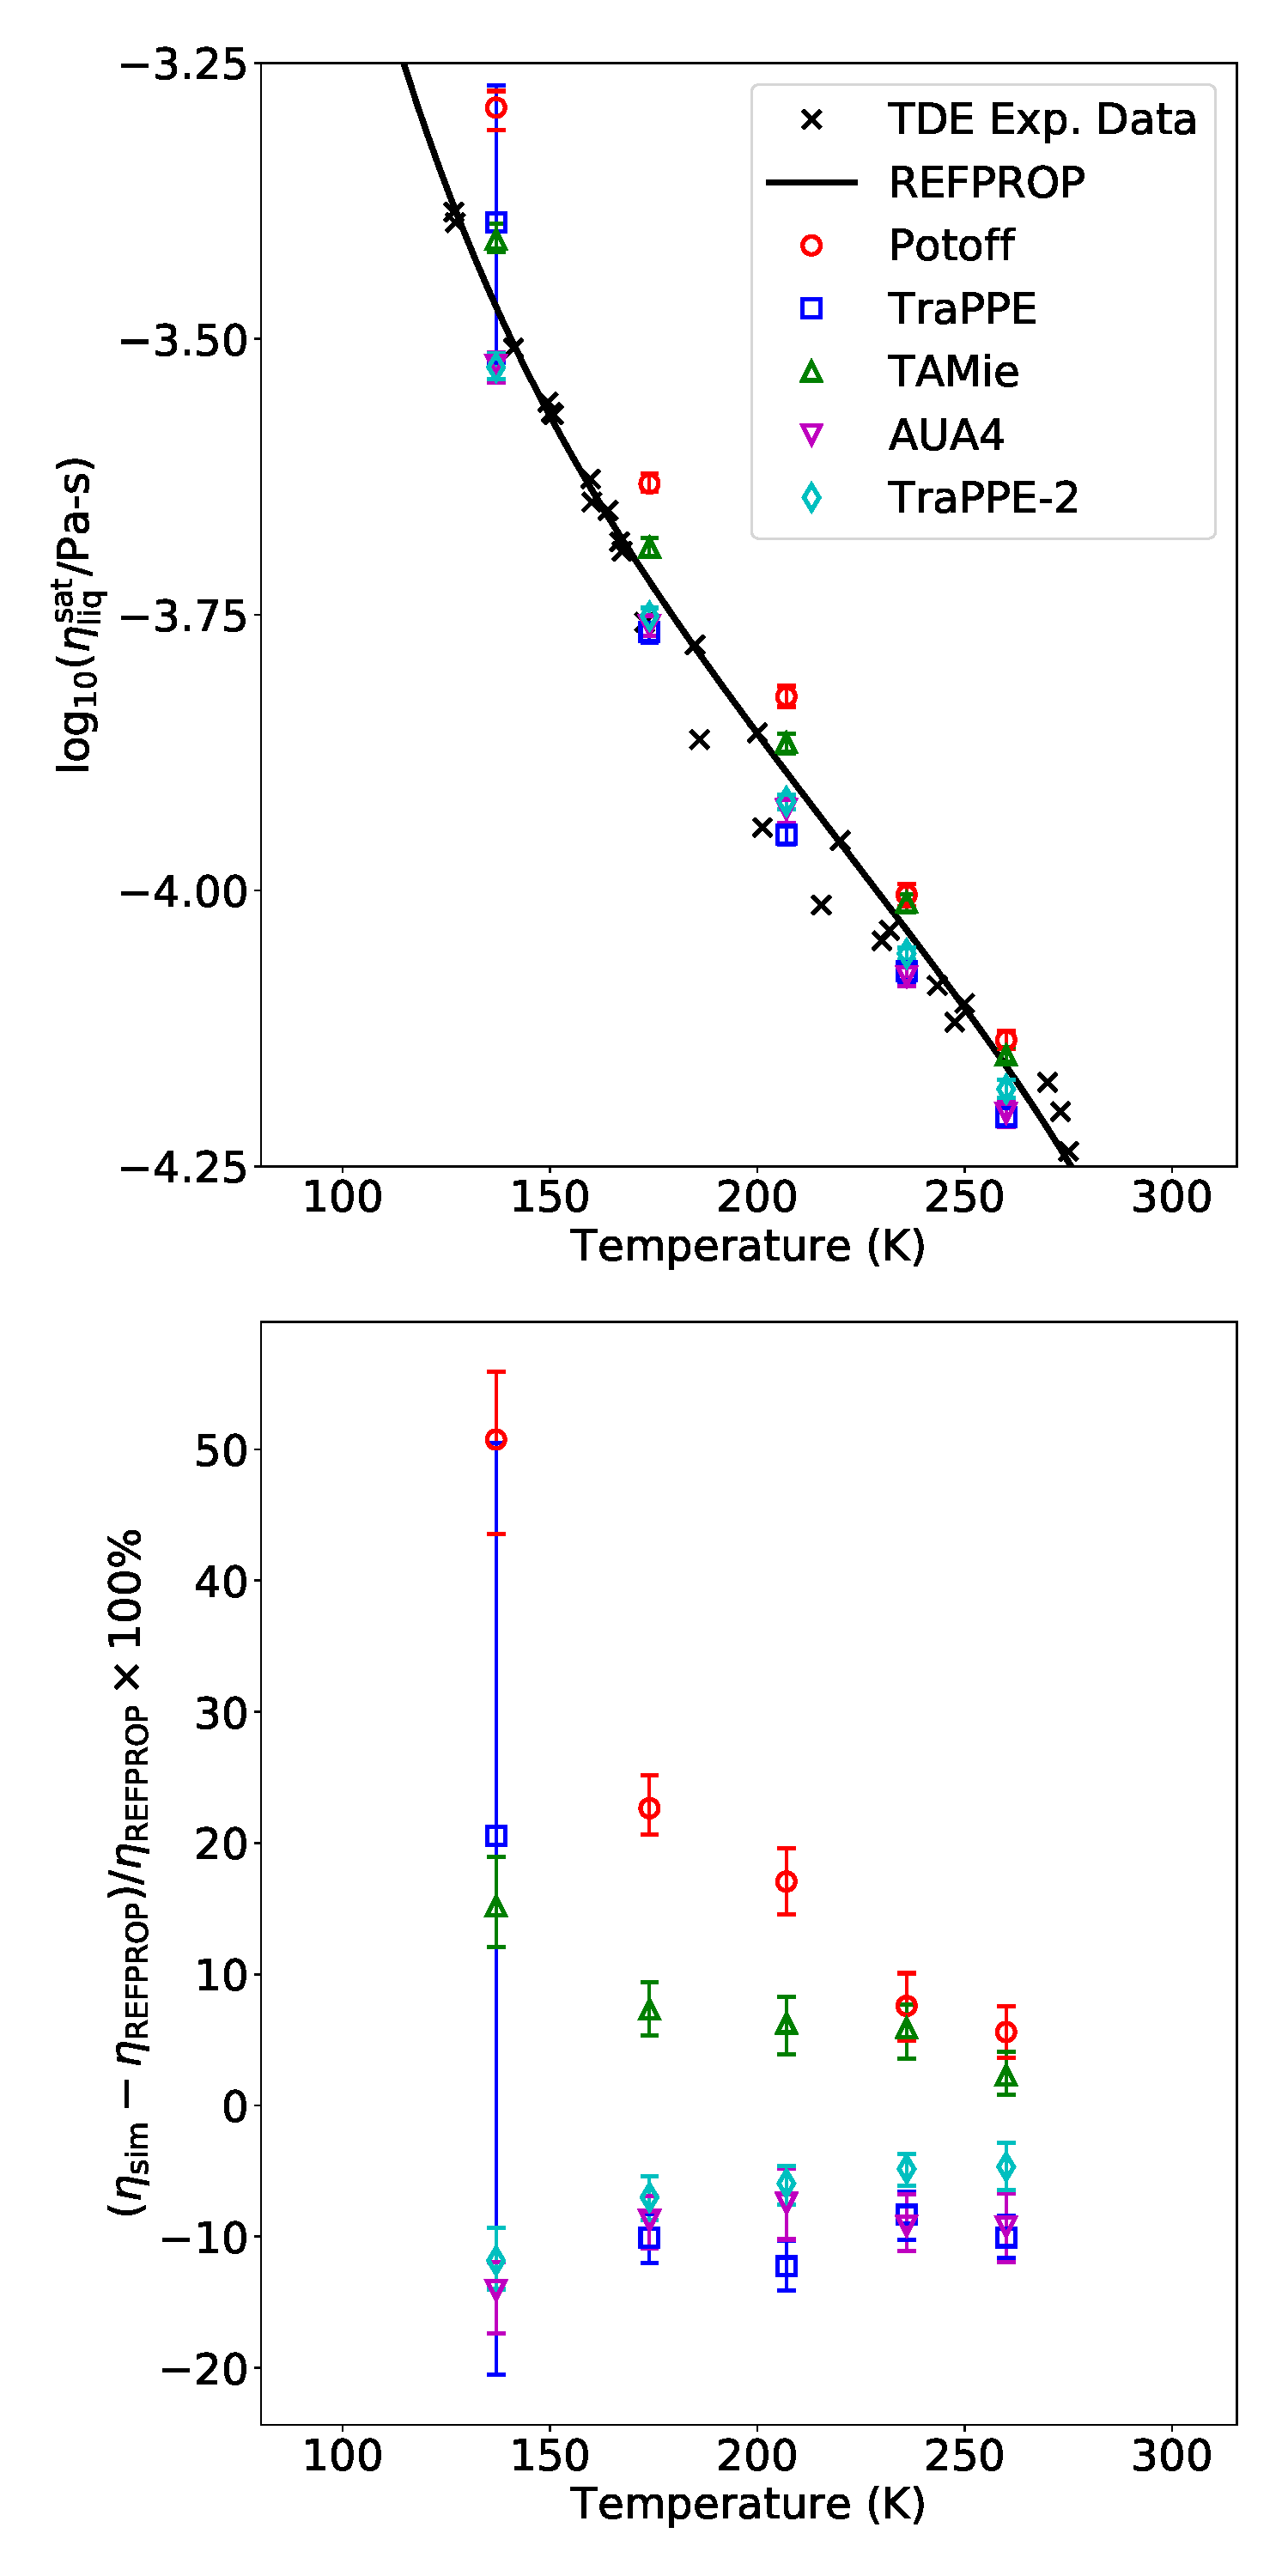
\includegraphics[width=3.2in]{compare_force_fields_ethane.pdf}
		\caption{Saturated liquid viscosities for ethane. Top panel compares simulation results with REFPROP correlations and experimental data available in TDE. Bottom panel presents percent deviations between simulated $(\eta_{\rm sim})$ and REFPROP $(\eta_{\rm REFPROP})$ values. Colors/symbols denote different force fields. Error bars represent the 95~\% confidence interval estimated with bootstrap re-sampling. When available, experimental uncertainties are typically smaller than one symbol size. Unless otherwise depicted, REFPROP uncertainties are smaller than the line-width.}
		\label{fig:Saturation_Ethane}
	\end{figure} 
	
	Figure \ref{fig:Saturation_C3_C4_C8} compares the TraPPE, Potoff, and TAMie saturated liquid viscosities for propane, \textit{n}-butane, and \textit{n}-octane. Similar to what has been demonstrated in previous studies, the TraPPE force field significantly under estimates $\eta_{\rm liq}^{\rm sat}$ (between 30 and 80~\%) with the deviation increasing with decreasing temperature \cite{Gordon2006,Nieto2006}. By contrast, the Potoff and TAMie force fields agree with the REFPROP values for these compounds to within 10~\%. Although TAMie deviations for propane increase to approximately 50~\% at the triple point temperature, Potoff deviations are nearly constant over the entire temperature range studied for each compound. 
	
	%By contrast, the Potoff and TAMie force fields agree with the REFPROP values for these compounds to within 10~\% over the entire temperature range studied (which includes the triple point for propane), and do not demonstrate a strong temperature dependence.
	
	\begin{figure}[htb!]
		\centering
		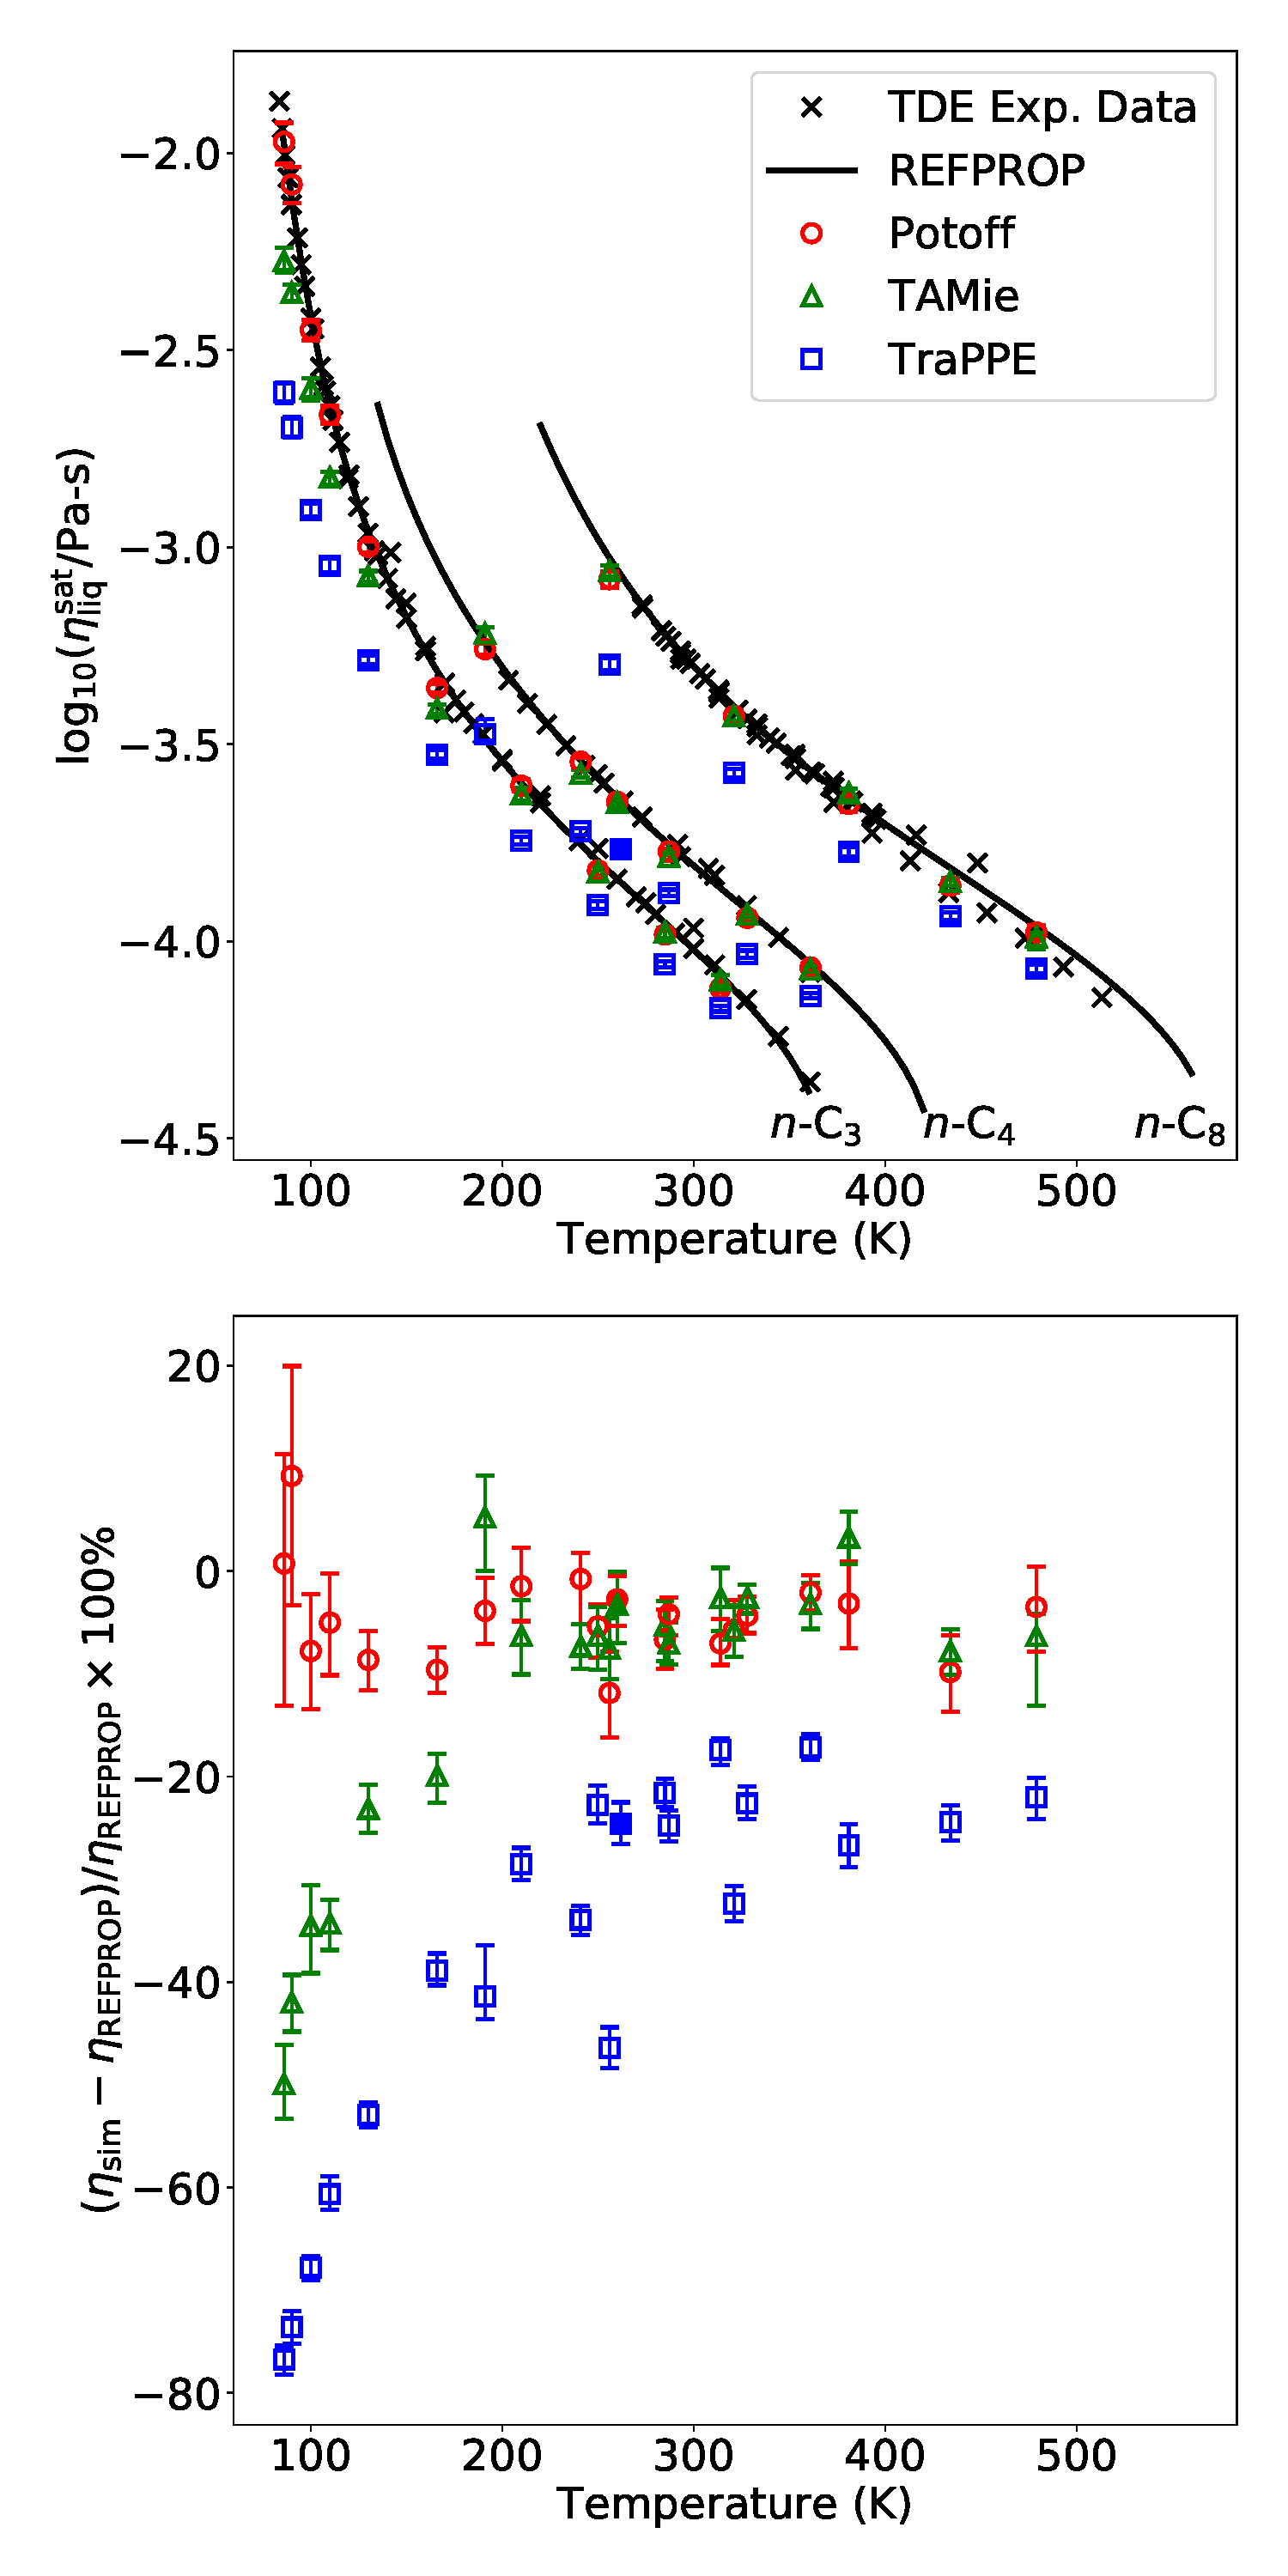
\includegraphics[width=3.2in]{compare_force_fields_short_normal.pdf}
		\caption{Saturated liquid viscosities for propane (\textit{n}-C$_{3}$), \textit{n}-butane (\textit{n}-C$_{4}$), and \textit{n}-octane (\textit{n}-C$_{8}$). See Figure \ref{fig:Saturation_Ethane} caption for details. Filled symbols correspond to simulations performed at the respective force field $\rho_{\rm liq}^{\rm sat}$ (see Section \ref{Discussion/Limitations}).}
		\label{fig:Saturation_C3_C4_C8}
	\end{figure} 
	
	Figure \ref{fig:Saturation_C12_C16_C22} compares the TraPPE, Potoff, and TAMie saturated liquid viscosities for \textit{n}-dodecane, \textit{n}-hexadecane, and \textit{n}-docosane. The TraPPE percent deviations for these compounds are similar to those observed in Figure \ref{fig:Saturation_C3_C4_C8} for smaller \textit{n}-alkanes. However, TAMie and Potoff percent deviations demonstrate a stronger temperature dependence for these larger \textit{n}-alkanes, i.e., the percent deviations increase with decreasing temperature. Although the cause of this trend is unclear, Section \ref{Discussion/Limitations} suggests that the cut-off distance impacts these larger compounds more than smaller compounds, especially at higher $\rho_{\rm liq}^{\rm sat}$ (lower $T^{\rm sat}$).
	
	%The cause of this trend is unclear but, since it is only observed for larger compounds, it is likely attributed to the torsional potential or the transferability of the CH$_2$ Mie $\lambda$-6 parameters.  
	
	\begin{figure}[htb!]
		\centering
		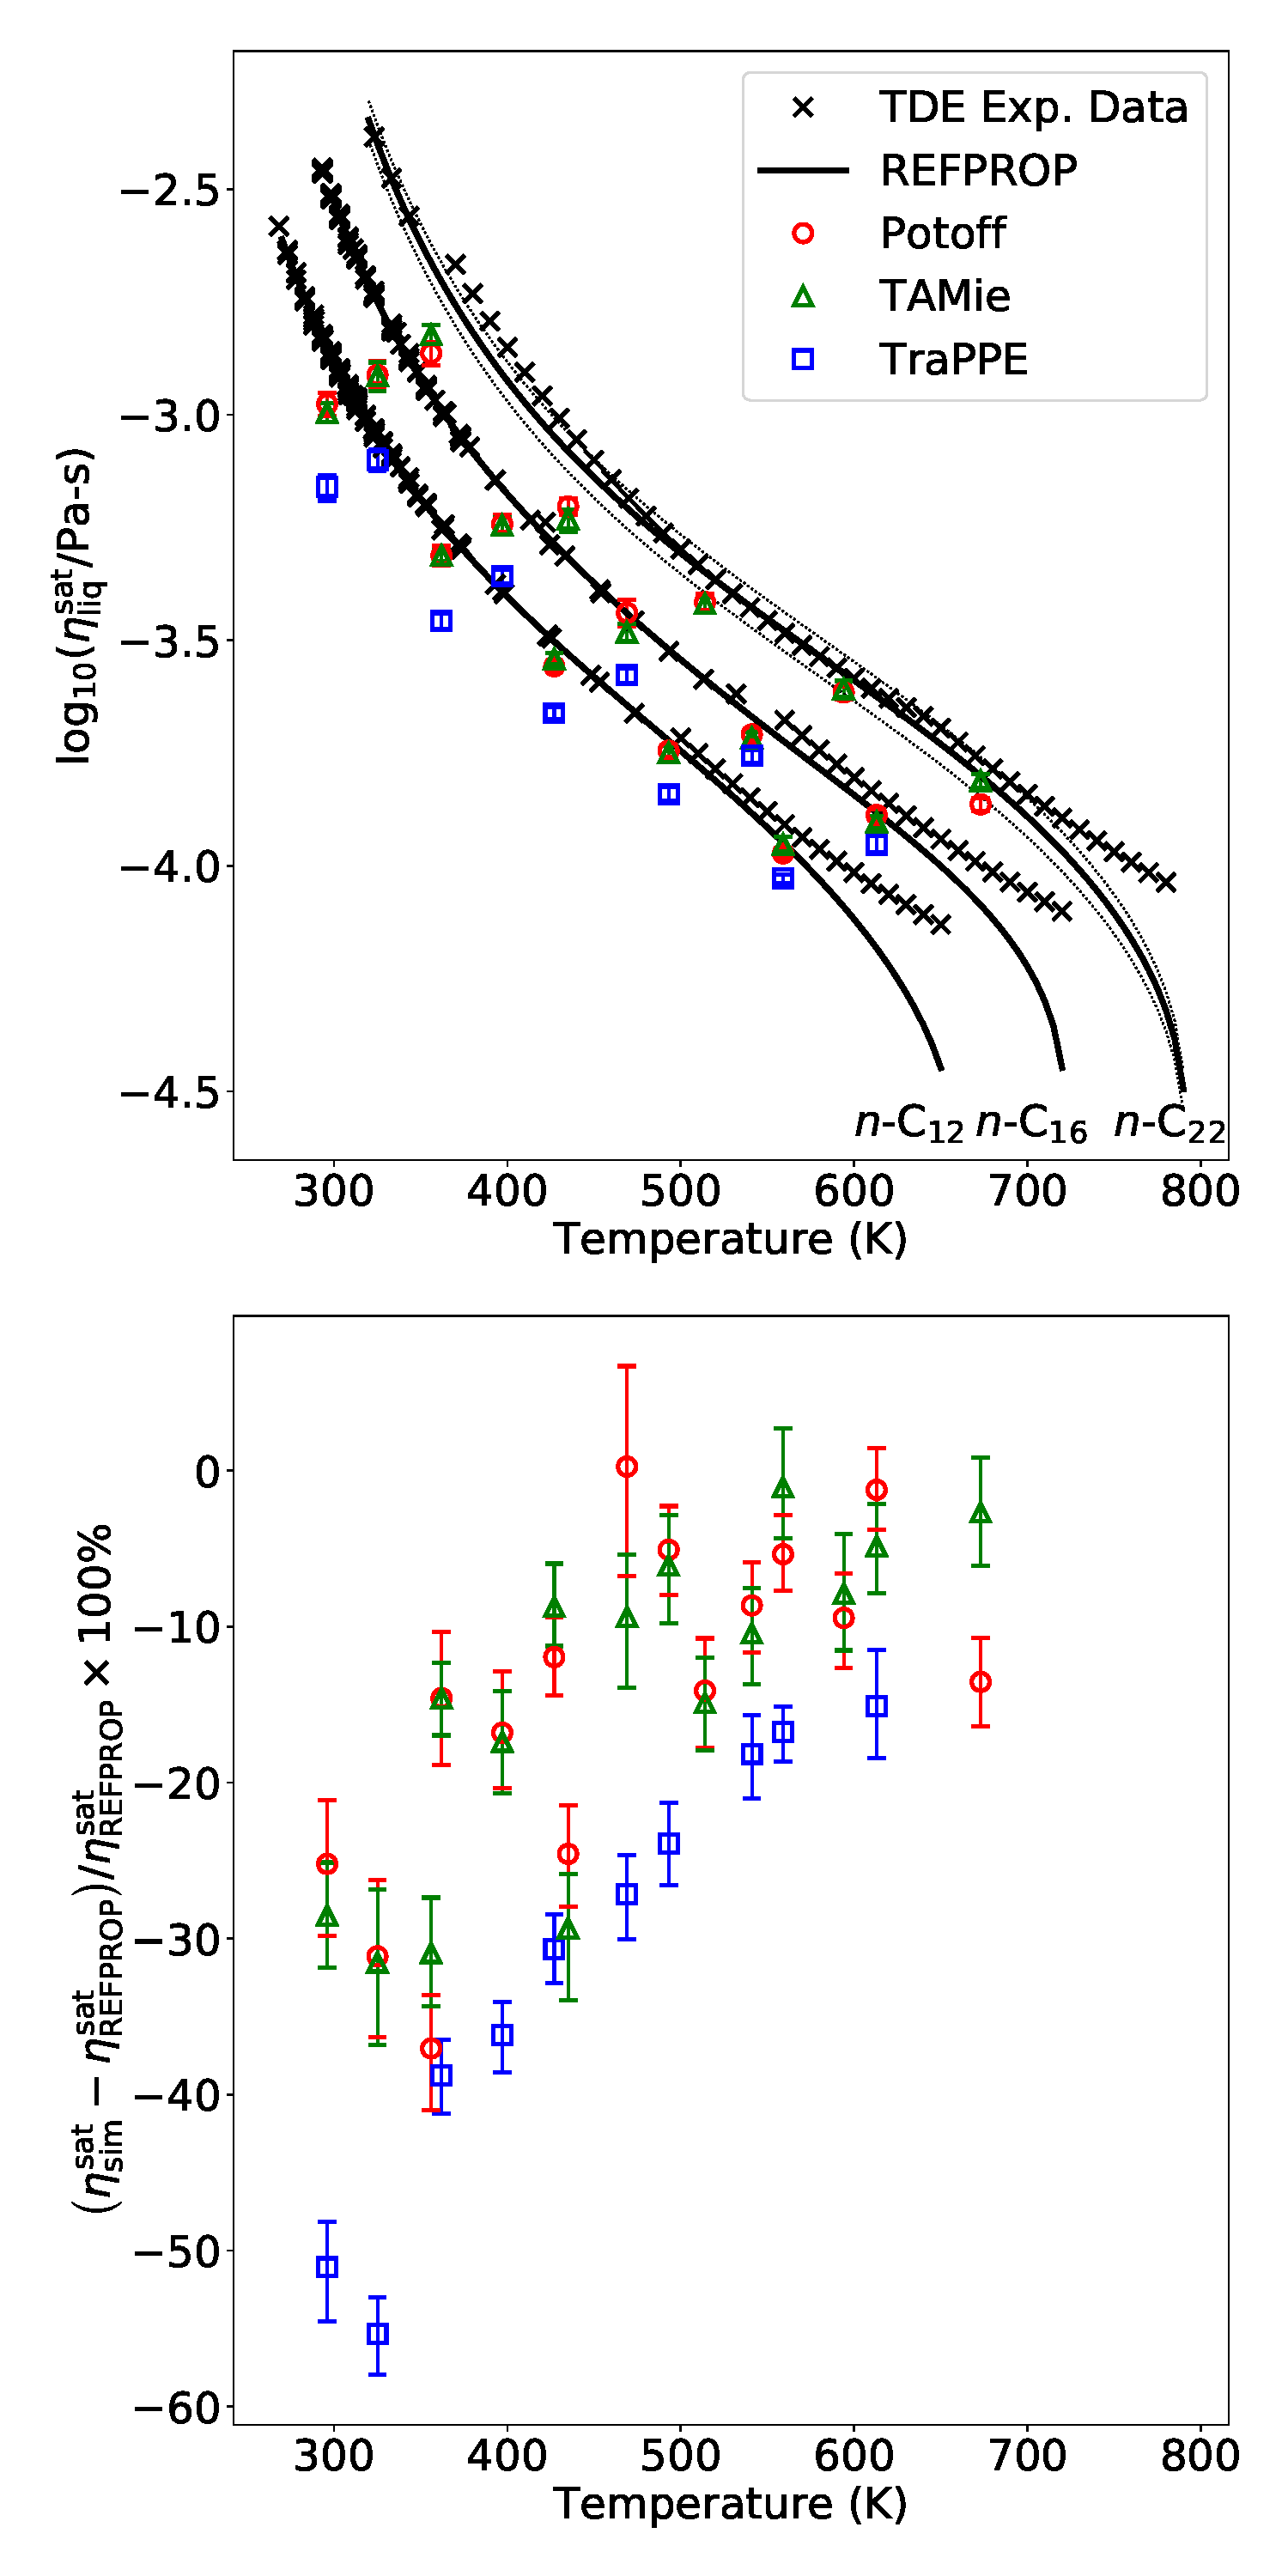
\includegraphics[width=3.2in]{compare_force_fields_long_normal.pdf}
		\caption{Saturated liquid viscosities for \textit{n}-dodecane (\textit{n}-C$_{12}$), \textit{n}-hexadecane (\textit{n}-C$_{16}$), and \textit{n}-docosane (\textit{n}-C$_{22}$). See Figure \ref{fig:Saturation_Ethane} caption for details.}
		\label{fig:Saturation_C12_C16_C22}
	\end{figure} 
	
	\subsubsection{Branched alkanes}
	
	%\begin{enumerate}
	%	\item Mie potential provides less improvement in these cases
	%\end{enumerate}
	
	%Figures:
	%
	%\begin{enumerate}
	%	\item IC4, NEOC5
	%	\item IC5, IC8
	%	\item IC6, 23DMB, 3MP
	%\end{enumerate}
	
	%Unfortunately, TAMie does not have parameters for C and, therefore, 
	
	%Figures \ref{fig:Saturation_IC4_NEOC5} to \ref{fig:Saturation_IC6_23DMB_3MP} compare the saturated liquid viscosities for each force field and branched alkane studied. Figure \ref{fig:Saturation_IC4_NEOC5} presents results for the more spherical compounds, namely, 2-methylpropane and 2,2-dimethylpropane. Figure \ref{fig:Saturation_IC5_IC8} presents results for a short and long chain, namely, 2-methylbutane and 2,2,4-trimethylpentane. Figure \ref{fig:Saturation_IC6_23DMB_3MP} presents results for various hexane isomers, namely, 2-methylpentane, 2,3-dimethylbutane, and 3-methylpentane. Each compound was simulated using the TraPPE (UA LJ 12-6) and Potoff (UA Mie 16-6) force fields. However, only 2-methylpropane and 2,2-dimethylpropane were simulated with AUA4 (AUA LJ 12-6) while 2,2-dimethylpropane and 2,2,4-trimethylpentane were not simulated using the TAMie (AUA Mie 14-6) force field.
	%
	%From Figure \ref{fig:Saturation_IC4_NEOC5} to \ref{fig:Saturation_IC6_23DMB_3MP}, we see that the Potoff S/L force field is not as accurate for the simulated branched alkanes as for the normal alkanes. However, it still provides considerable improvement compared to the LJ 12-6 based models, i.e., TraPPE and AUA4. Surprisingly, the TAMie force field performs much worse for these branched alkanes. 
	%
	%%Figure \ref{fig:Saturation_IC4_NEOC5} compares the TraPPE (UA LJ 12-6), AUA4 (AUA LJ 12-6), and Potoff (UA Mie 16-6) saturated liquid viscosities for 2-methylpropane and 2,2-dimethylpropane.
	%
	%\begin{figure}[p!]
	%	\centering
	%	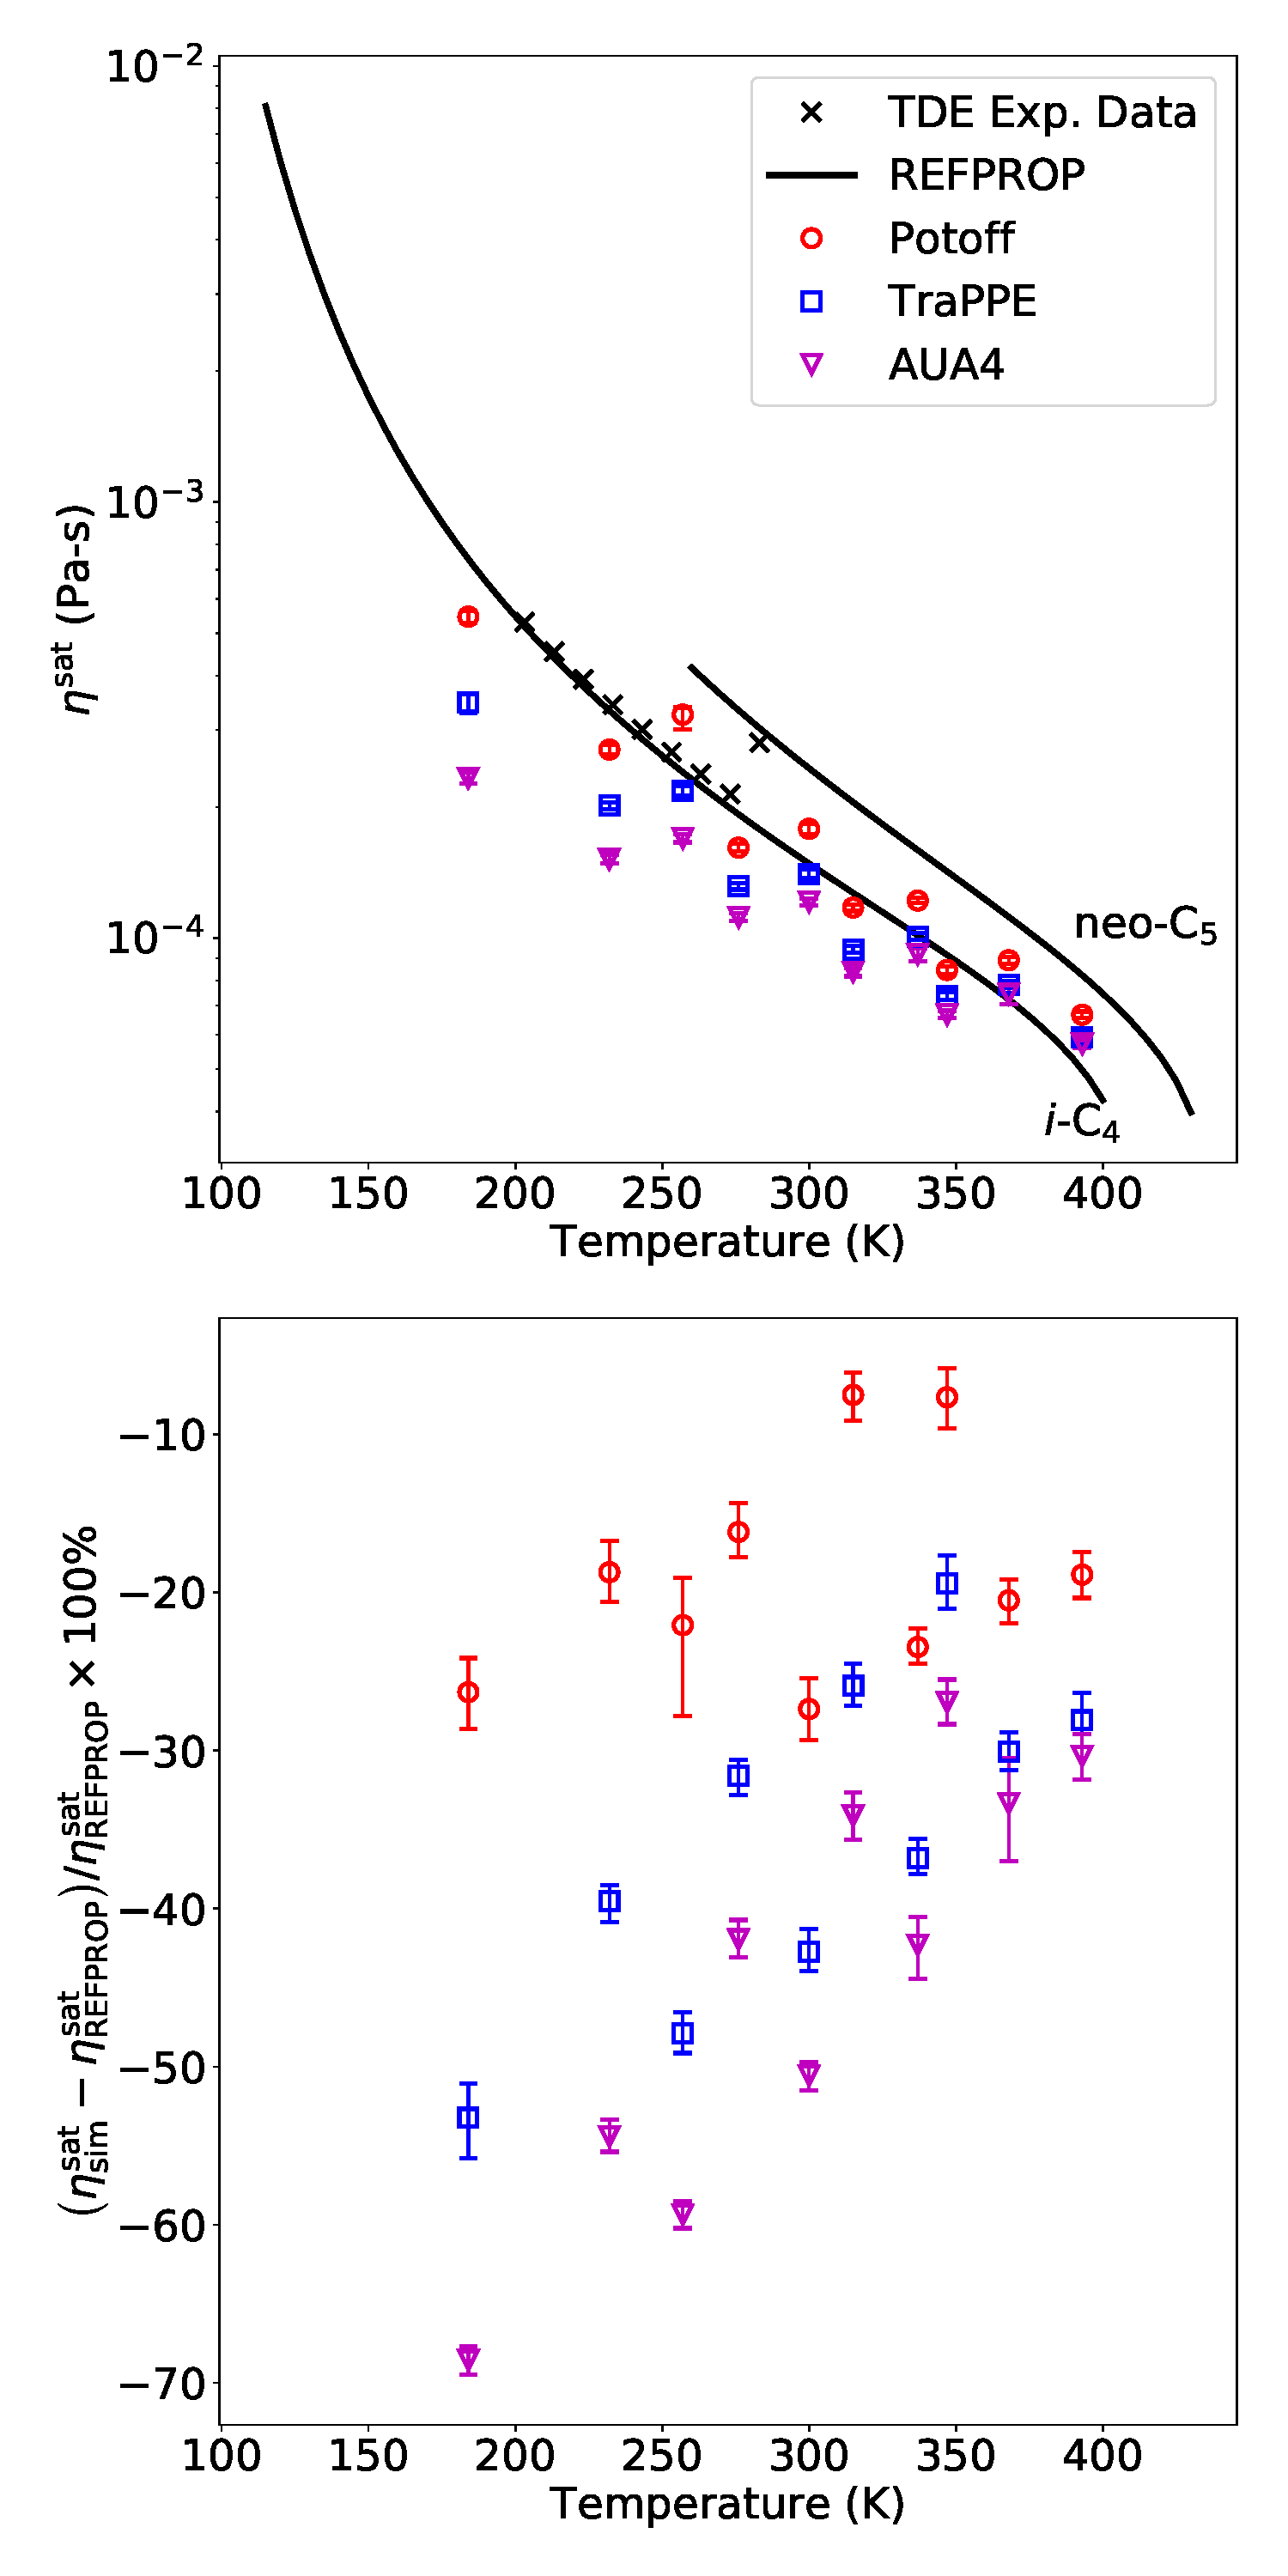
\includegraphics[width=3.2in]{compare_force_fields_IC4_neoC5.pdf}
	%	\caption{Saturated liquid viscosities for 2-methylpropane and 2,2-dimethylpropane. Colors/symbols denote different force fields.}
	%	\label{fig:Saturation_IC4_NEOC5}
	%\end{figure} 
	%
	%%Figure \ref{fig:Saturation_IC5_IC8} compares the TraPPE, Potoff, and TAMie saturated liquid viscosities for 2-methylbutane and 2,2,4-trimethylpentane.
	%
	%\begin{figure}[p!]
	%	\centering
	%	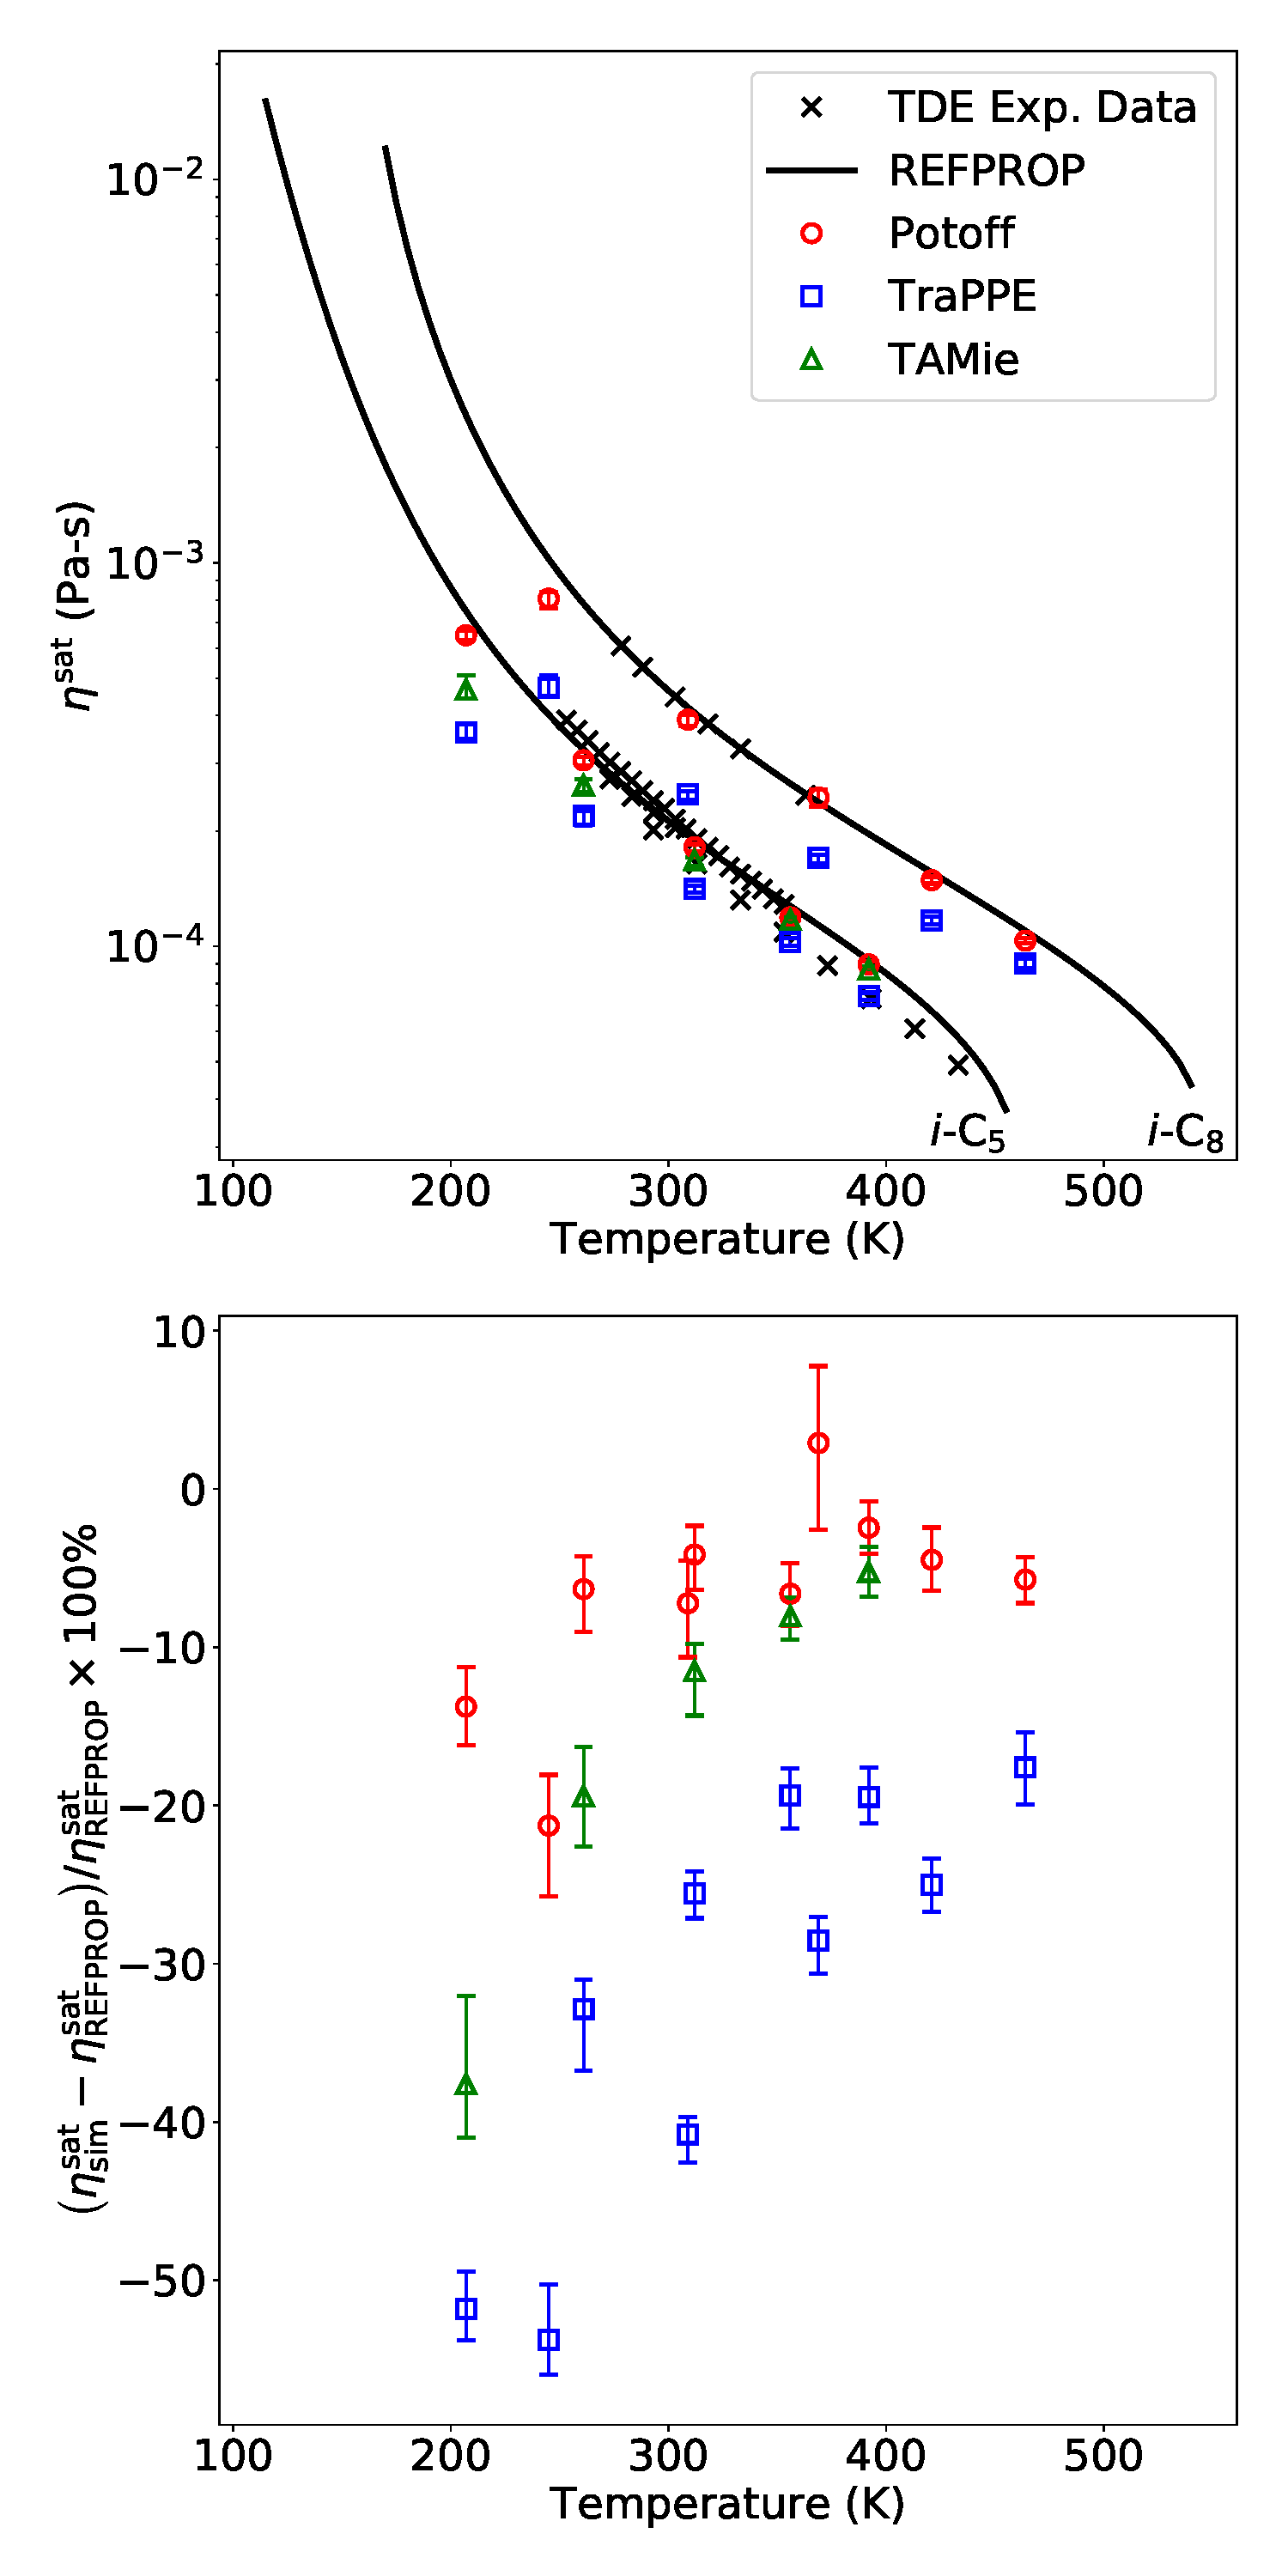
\includegraphics[width=3.2in]{compare_force_fields_IC5_IC8.pdf}
	%	\caption{Saturated liquid viscosities for 2-methylbutane and 2,2,4-trimethylpentane. Colors/symbols denote different force fields.}
	%	\label{fig:Saturation_IC5_IC8}
	%\end{figure} 
	%
	%%Figure \ref{fig:Saturation_IC6_23DMB_3MP} compares the TraPPE, Potoff, and TAMie saturated liquid viscosities for 2-methylbutane and 2,2,4-trimethylpentane.
	%
	%\begin{figure}[p!]
	%	\centering
	%	
\includegraphics[width=3.2in]{empty_figure.jpg}
	%	\caption{Saturated liquid viscosities for 2-methylpentane, 2,3-dimethylbutane, and 3-methylpentane. Colors/symbols denote different force fields.}
	%	\label{fig:Saturation_IC6_23DMB_3MP}
	%\end{figure}
	
	Figures \ref{fig:Saturation_short_branched} and \ref{fig:Saturation_long_branched} compare the saturated liquid viscosities for branched alkanes. Figures \ref{fig:Saturation_short_branched} and \ref{fig:Saturation_long_branched} present results for the compounds classified by Potoff as ``short'' and ``long'', respectively \cite{Mie}. Specifically, Figure \ref{fig:Saturation_short_branched} depicts 2-methylpropane, 2,2-dimethylpropane, 2-methylbutane, and 2,3-dimethylbutane, while Figure \ref{fig:Saturation_long_branched} contains 2-methylpentane, 3-methylpentane, and 2,2,4-trimethylpentane. Each compound was simulated using the TraPPE and Potoff force fields. However, only 2,2-dimethylpropane was simulated with AUA4 while 2,2-dimethylpropane and 2,2,4-trimethylpentane were not simulated using the TAMie force field.
	
	%From Figure \ref{fig:Saturation_IC4_NEOC5} to \ref{fig:Saturation_IC6_23DMB_3MP}, we see that the Potoff S/L force field is not as accurate for the simulated branched alkanes as for the normal alkanes. However, it still provides considerable improvement compared to the LJ 12-6 based models, i.e., TraPPE and AUA4. Surprisingly, the TAMie force field performs much worse for these branched alkanes. 
	
	\begin{figure}[htb!]
		\centering
		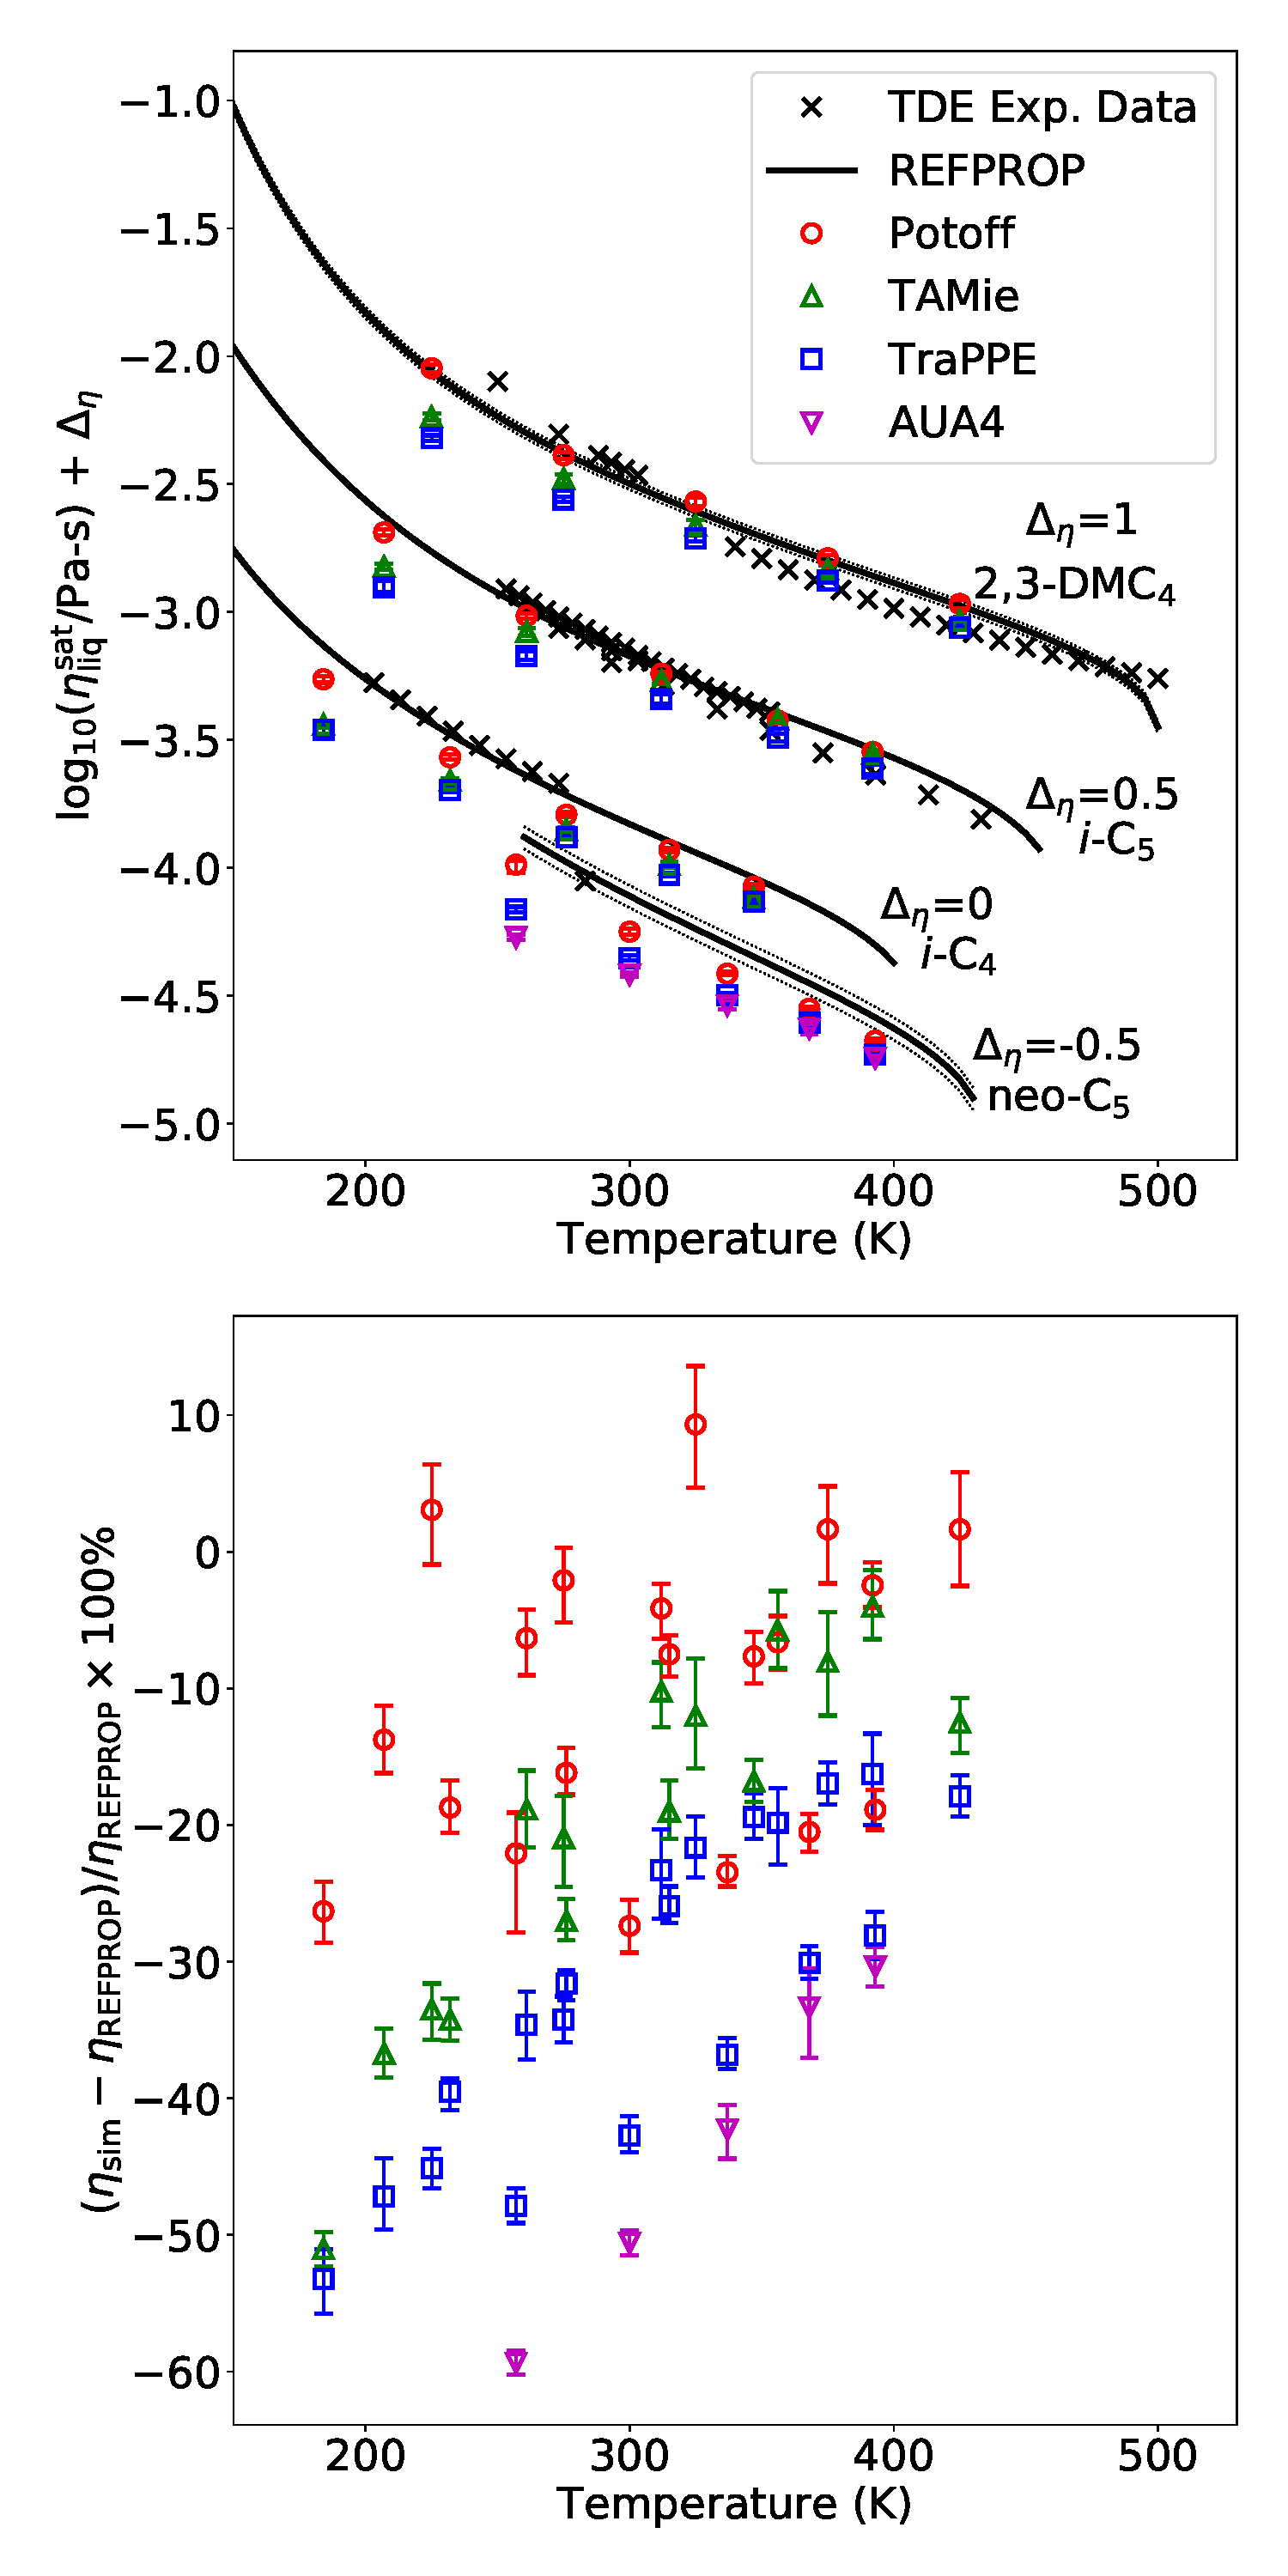
\includegraphics[width=3.2in]{compare_force_fields_short_branched.pdf}
		\caption{Saturated liquid viscosities for 2-methylpropane (\textit{i}-C$_{4}$), 2,2-dimethylpropane (neo-C$_{5}$), 2-methylbutane (\textit{i}-C$_{5}$), and 2,3-dimethylbutane (2,3-DMC$_4$). See Figure \ref{fig:Saturation_Ethane} caption for details. For clarity, values in top panel are shifted by $\Delta \eta$.}
		\label{fig:Saturation_short_branched}
	\end{figure} 
	
	\begin{figure}[htb!]
		\centering
		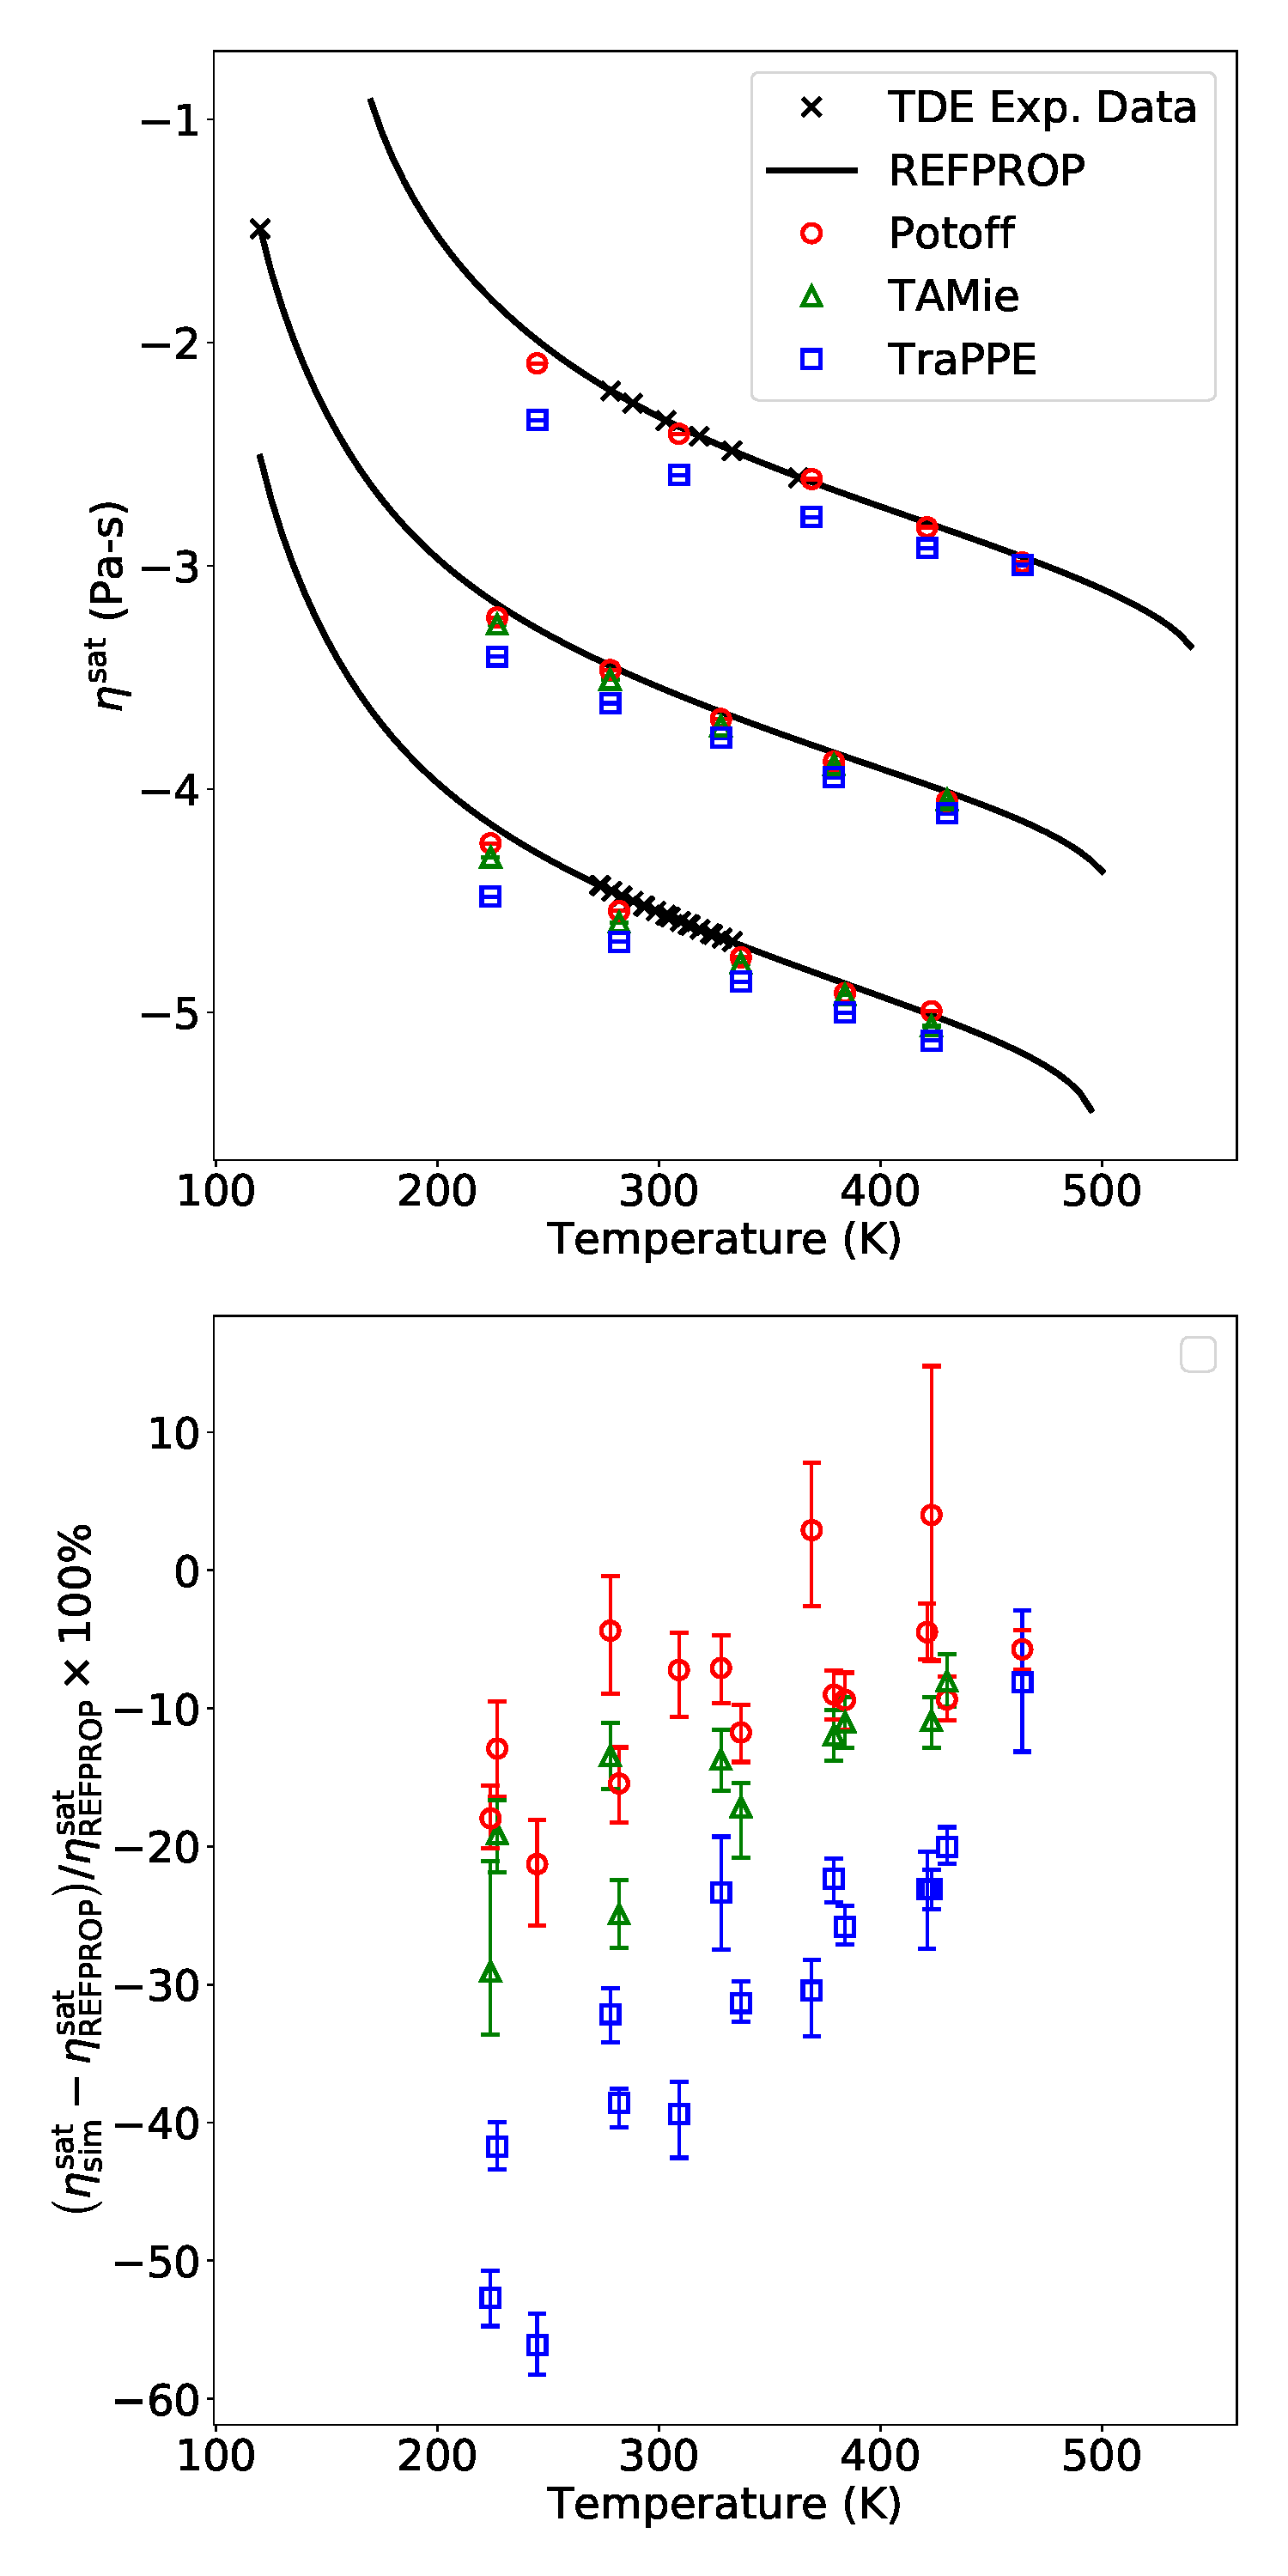
\includegraphics[width=3.2in]{compare_force_fields_long_branched.pdf}
		\caption{Saturated liquid viscosities for 2-methylpentane (\textit{i}-C$_{6}$), 3-methylpentane (3-MC$_5$), and 2,2,4-trimethylpentane (\textit{i}-C$_{8}$). See Figure \ref{fig:Saturation_Ethane} caption for details. For clarity, values in top panel are shifted by $\Delta \eta$. Filled symbols correspond to simulations performed at the respective force field $\rho_{\rm liq}^{\rm sat}$ (see Section \ref{Discussion/Limitations}).}
		\label{fig:Saturation_long_branched}
	\end{figure} 
	
	From Figures \ref{fig:Saturation_short_branched} and \ref{fig:Saturation_long_branched}, we see that the Potoff S/L and TAMie force fields are not as accurate for these branched alkanes as for the normal alkanes. In particular, Potoff and TAMie deviations demonstrate the same temperature dependence observed for other force fields, where the percent deviations are largest at lower temperatures. However, Potoff still provides considerable improvement compared to the LJ 12-6 based models, i.e., TraPPE and AUA4. Note that the Potoff ``short'' and ``long'' parameters in Figures \ref{fig:Saturation_short_branched} and \ref{fig:Saturation_long_branched}, respectively, provide similar accuracy. 
	
	%The one apparent exception is 3-methylpentane, where the Potoff deviations are less than 10~\% over the entire temperature range. However, considering the availabi 
	
	The deviations for each force field are largest for 2-methylpropane and 2,2-dimethylpropane, the two smallest and most spherical branched alkanes. Since these compounds are primarily composed of CH$_3$ UA sites, this poor performance is likely due to the assumption that the CH$_3$ non-bonded parameters are transferable from \textit{n}-alkanes to branched alkanes. Improvement might be possible if the CH$_3$ parameters were different depending on the neighboring UA site type. However, it is also important to note that the 2,2-dimethylpropane REFPROP viscosity correlation is not considered to be of ``reference quality.''
	
	\subsection{Compressed liquid} \label{sec:T293highP}
	
	Section \ref{sec:eta_sat} demonstrates that Mie $\lambda$-6 based force fields (Potoff and TAMie) are considerably more reliable for predicting saturated liquid viscosities than LJ 12-6 based force fields (TraPPE and AUA4). However, as the Mie $\lambda$-6 potential is too repulsive at short distances for $\lambda > 12$, the Potoff (Mie 16-6) and TAMie (Mie 14-6) force fields tend to over estimate pressure at high densities \cite{Postdoc_2}. Since $\eta$ also increases with larger values of $\lambda$, our \textit{ansatz} is that Potoff and TAMie should over estimate $\eta$ at high densities/pressures. 
	
	Surprisingly, Gordon shows that a (slightly modified) Mie 14-6 (for CH$_3$) and Mie 20-6 (for CH$_2$) potential can accurately predict the $\eta$-$P$ dependence for \textit{n}-hexadecane up to 400 MPa \cite{Gordon2006}. Since the Gordon force field was parameterized with $\eta_{\rm liq}^{\rm sat}$ data, the purpose of this section is to determine if the Potoff and TAMie force fields, which did not include viscosity data in their parameterization, are also reliable for estimating the $\eta$-$P$ dependence. To provide additional insight into the consequences of using a Mie $\lambda$-6 potential with $\lambda > 12$, we present results for the $\eta$-$\rho$ dependence as well (which was not reported by Gordon). 
	
%	Note that Reference \citenum{Gordon2006} did not report the $\eta$-$\rho$ dependence, utilizes a slightly modified Mie formulation, and included saturated liquid viscosity data in the non-bonded parameterization.
	
%	 a more repulsive potential (larger values of $\lambda$) increases visc
	
%	 since the Mie 16-6 and 14-6 potentials of Potoff and TAMie, respectively, are too repulsive at short distances,
%	
%	due to their overly repulsive Mie 14-6 and 16-6 potentials Reference \citenum{Postdoc_2} confirms that the Mie $\lambda$-6 potential is too repulsive at short distances for $\lambda > 12$, which causes the Potoff (16-6) and TAMie (14-6) force fields to over estimate pressure at high densities.
%	
%	Recently, it was shown that the Mie 14-6 and 16-6 potentials of TAMie and Potoff, respectively, are overly repulsive at high densities/pressures.
%	
	%However, Reference \citenum{Postdoc_2} confirms that the Mie $\lambda$-6 potential is too repulsive at short distances for $\lambda > 12$, which causes the Potoff (16-6) and TAMie (14-6) force fields to over estimate pressure at high densities.
	
%	Note that both the Potoff and TAMie non-bonded potentials use $\lambda > 12$.
	
	% Note that Reference \citenum{Gordon2006} utilized a slightly modified version of the Mie potential
	
	%The purpose of this section is to determine if a similar phenomenon is observed for viscosity estimates at high densities/pressures along the isotherm of 293 K.
	
	%The purpose of this section is to determine if a similar phenomenon is observed for viscosity estimates at high densities/pressures along the isotherm of 293 K. 
	
	\subsubsection{Normal alkanes}
	
%	\begin{enumerate}
%		\item Propane has accurate viscosity-P but not viscosity-rho
%		\item Butane appears to agree more closely with recent REFPROP correlation
%	\end{enumerate}
	
	%Figures:
	%
	%\begin{enumerate}
	%	\item Propane $\eta-\rho$ $\eta-P$
	%	\item Butane $\eta-\rho$ $\eta-P$
	%	\item n-Octane $\eta-\rho$ $\eta-P$
	%	%	\item n-Dodecane $\eta-\rho$ $\eta-P$?
	%\end{enumerate}
	
	Figures \ref{fig:T293highP_C3}, \ref{fig:T293highP_C4}, and \ref{fig:T293highP_C8} present the compressed liquid viscosities $(\eta_{\rm liq}^{\rm comp})$ for propane, \textit{n}-butane, and \textit{n}-octane, respectively. Each compound is simulated using the TraPPE, Potoff, and TAMie force fields at various densities. Simulation results are compared with REFPROP correlations and TDE data, when available. 
	
%	All TDE data for temperatures between 288 K and 298 K are depicted. REFPROP uncertainties are assumed to be a constant percent deviation as reported in the corresponding publication. ``REFPROP extrapolation'' are values that are found outside of the ``reference quality'' range. This extrapolation is intended to guide the eye when comparing with simulation results at high densities/pressures.
	
	% Note that for propane and \textit{n}-butane (Figures \ref{fig:T293highP_C3} and \ref{fig:T293highP_C4}) each force field is simulated at the same density, while for \textit{n}-octane (Figure \ref{fig:T293highP_C8}) the force fields are simulated at the same pressure. 
	
	%As the REFPROP viscosity correlation is not recommended above 100 MPa at 293 K, we have plotted some experimental data to guide the eye.
	
	\begin{figure}[H]
		\centering
		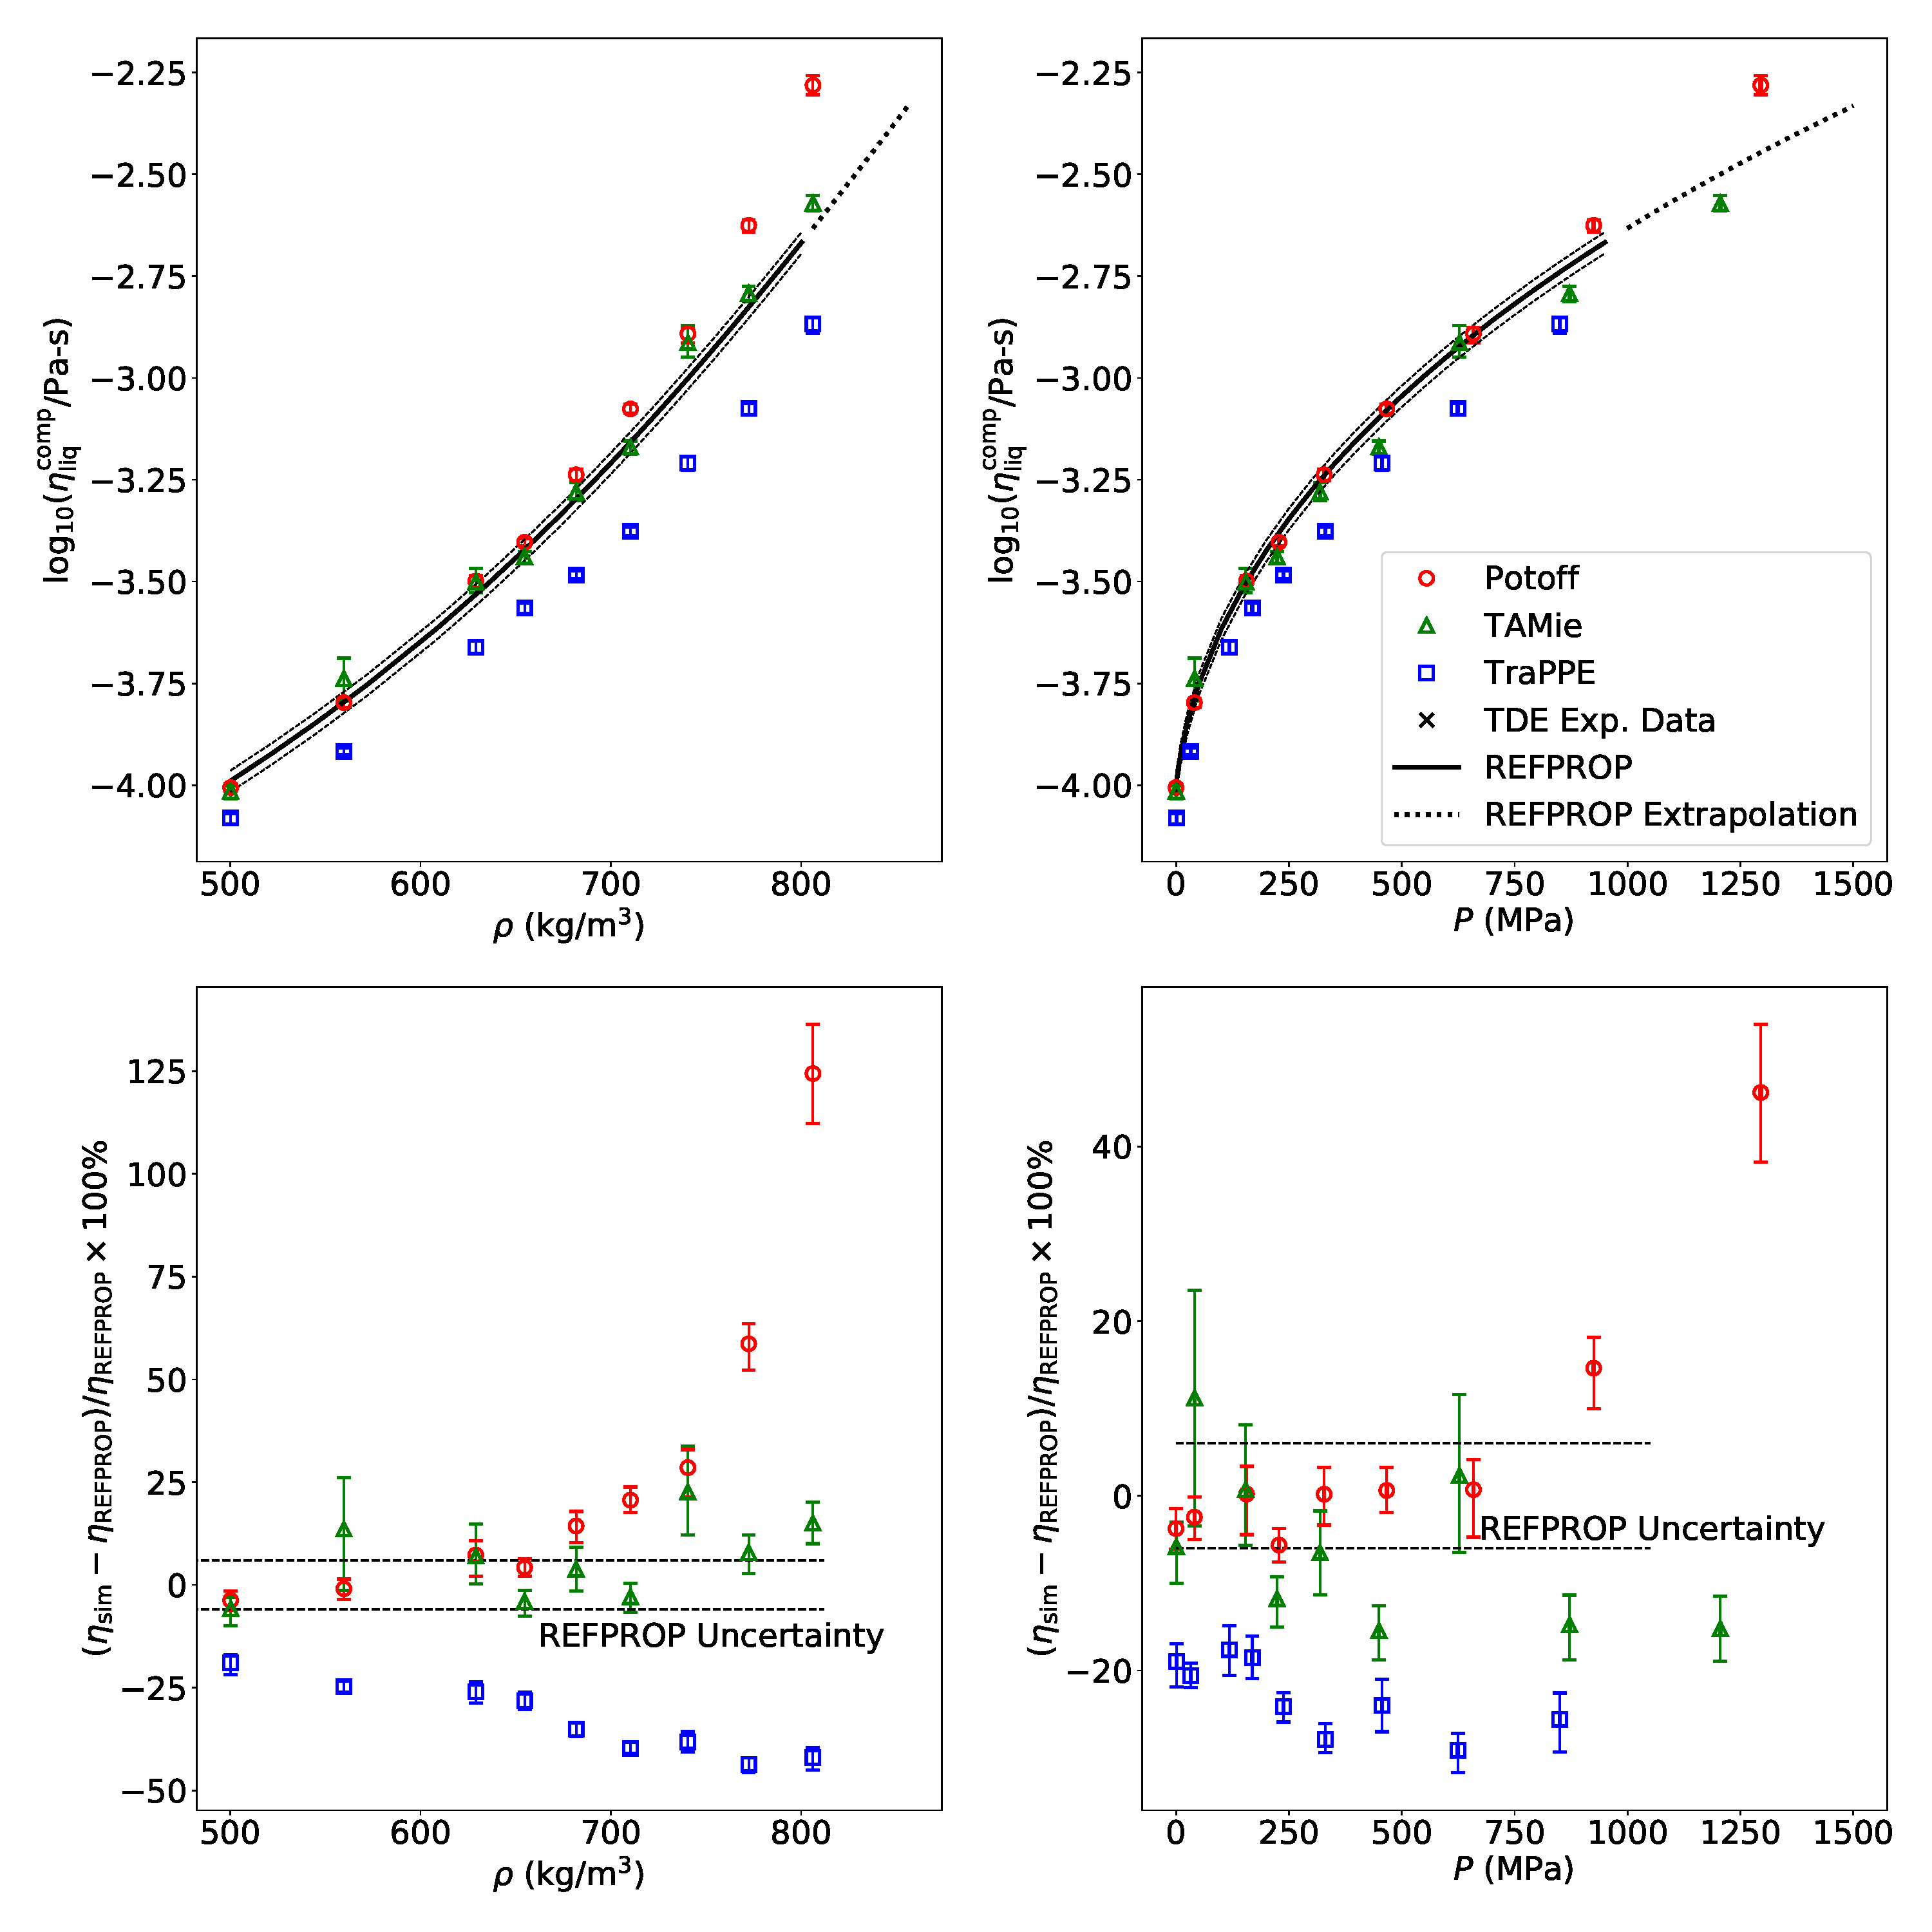
\includegraphics[width=6.4in]{compare_REFPROP_T293highP_C3H8.pdf}
		\caption{Compressed liquid viscosities at 293 K for propane. Top panels provide $\eta$-$\rho$ and $\eta$-$P$ dependence. Bottom panels present percent deviations between simulated $(\eta_{\rm sim})$ and REFPROP $(\eta_{\rm REFPROP})$ values with respect to $\rho$ and $P$. TDE data for temperatures between 288 and 298 K are depicted when available. Dashed lines correspond to reported REFPROP uncertainties. Dotted lines are extrapolation values outside of ``reference quality'' range, intended to guide the eye when comparing with simulation results at high densities/pressures. Colors/symbols denote different force fields and experimental data. Error bars represent the 95~\% confidence interval estimated with bootstrap re-sampling.}
		\label{fig:T293highP_C3}
	\end{figure} 

% Simulation uncertainties are obtained from bootstrap re-sampling and are presented at the 95~\% confidence level.
	
	Figures \ref{fig:T293highP_C3}, \ref{fig:T293highP_C4}, and \ref{fig:T293highP_C8} demonstrate that the TraPPE force field has a constant negative bias even with increasing density/pressure. The TAMie force field has the most accurate $\eta$-$\rho$ dependence, i.e., the error does not increase significantly with respect to density. By contrast, the Potoff potential demonstrates considerable over estimation of $\eta$ at high densities, which is likely attributed to the overly repulsive Mie 16-6 potential at close distances. Remarkably, the Potoff force field is the most accurate at predicting the $\eta$-$P$ dependence from saturation to elevated pressures (approaching 1000 MPa). This can be explained as a cancellation of errors since the Potoff force field significantly over predicts both $\eta$ and $P$ at high densities. Note that the increase in Potoff deviations for the two highest pressures in Figure \ref{fig:T293highP_C3} can potentially be explained by the large uncertainty in the REFPROP correlation and dubious extrapolation at these extreme pressures. Therefore, although Potoff should not be used to estimate the $\eta$-$\rho$ dependence, we conclude that it is the most reliable force field for estimating the $\eta$-$P$ dependence.
	
	\begin{figure}[htb!]
		\centering
		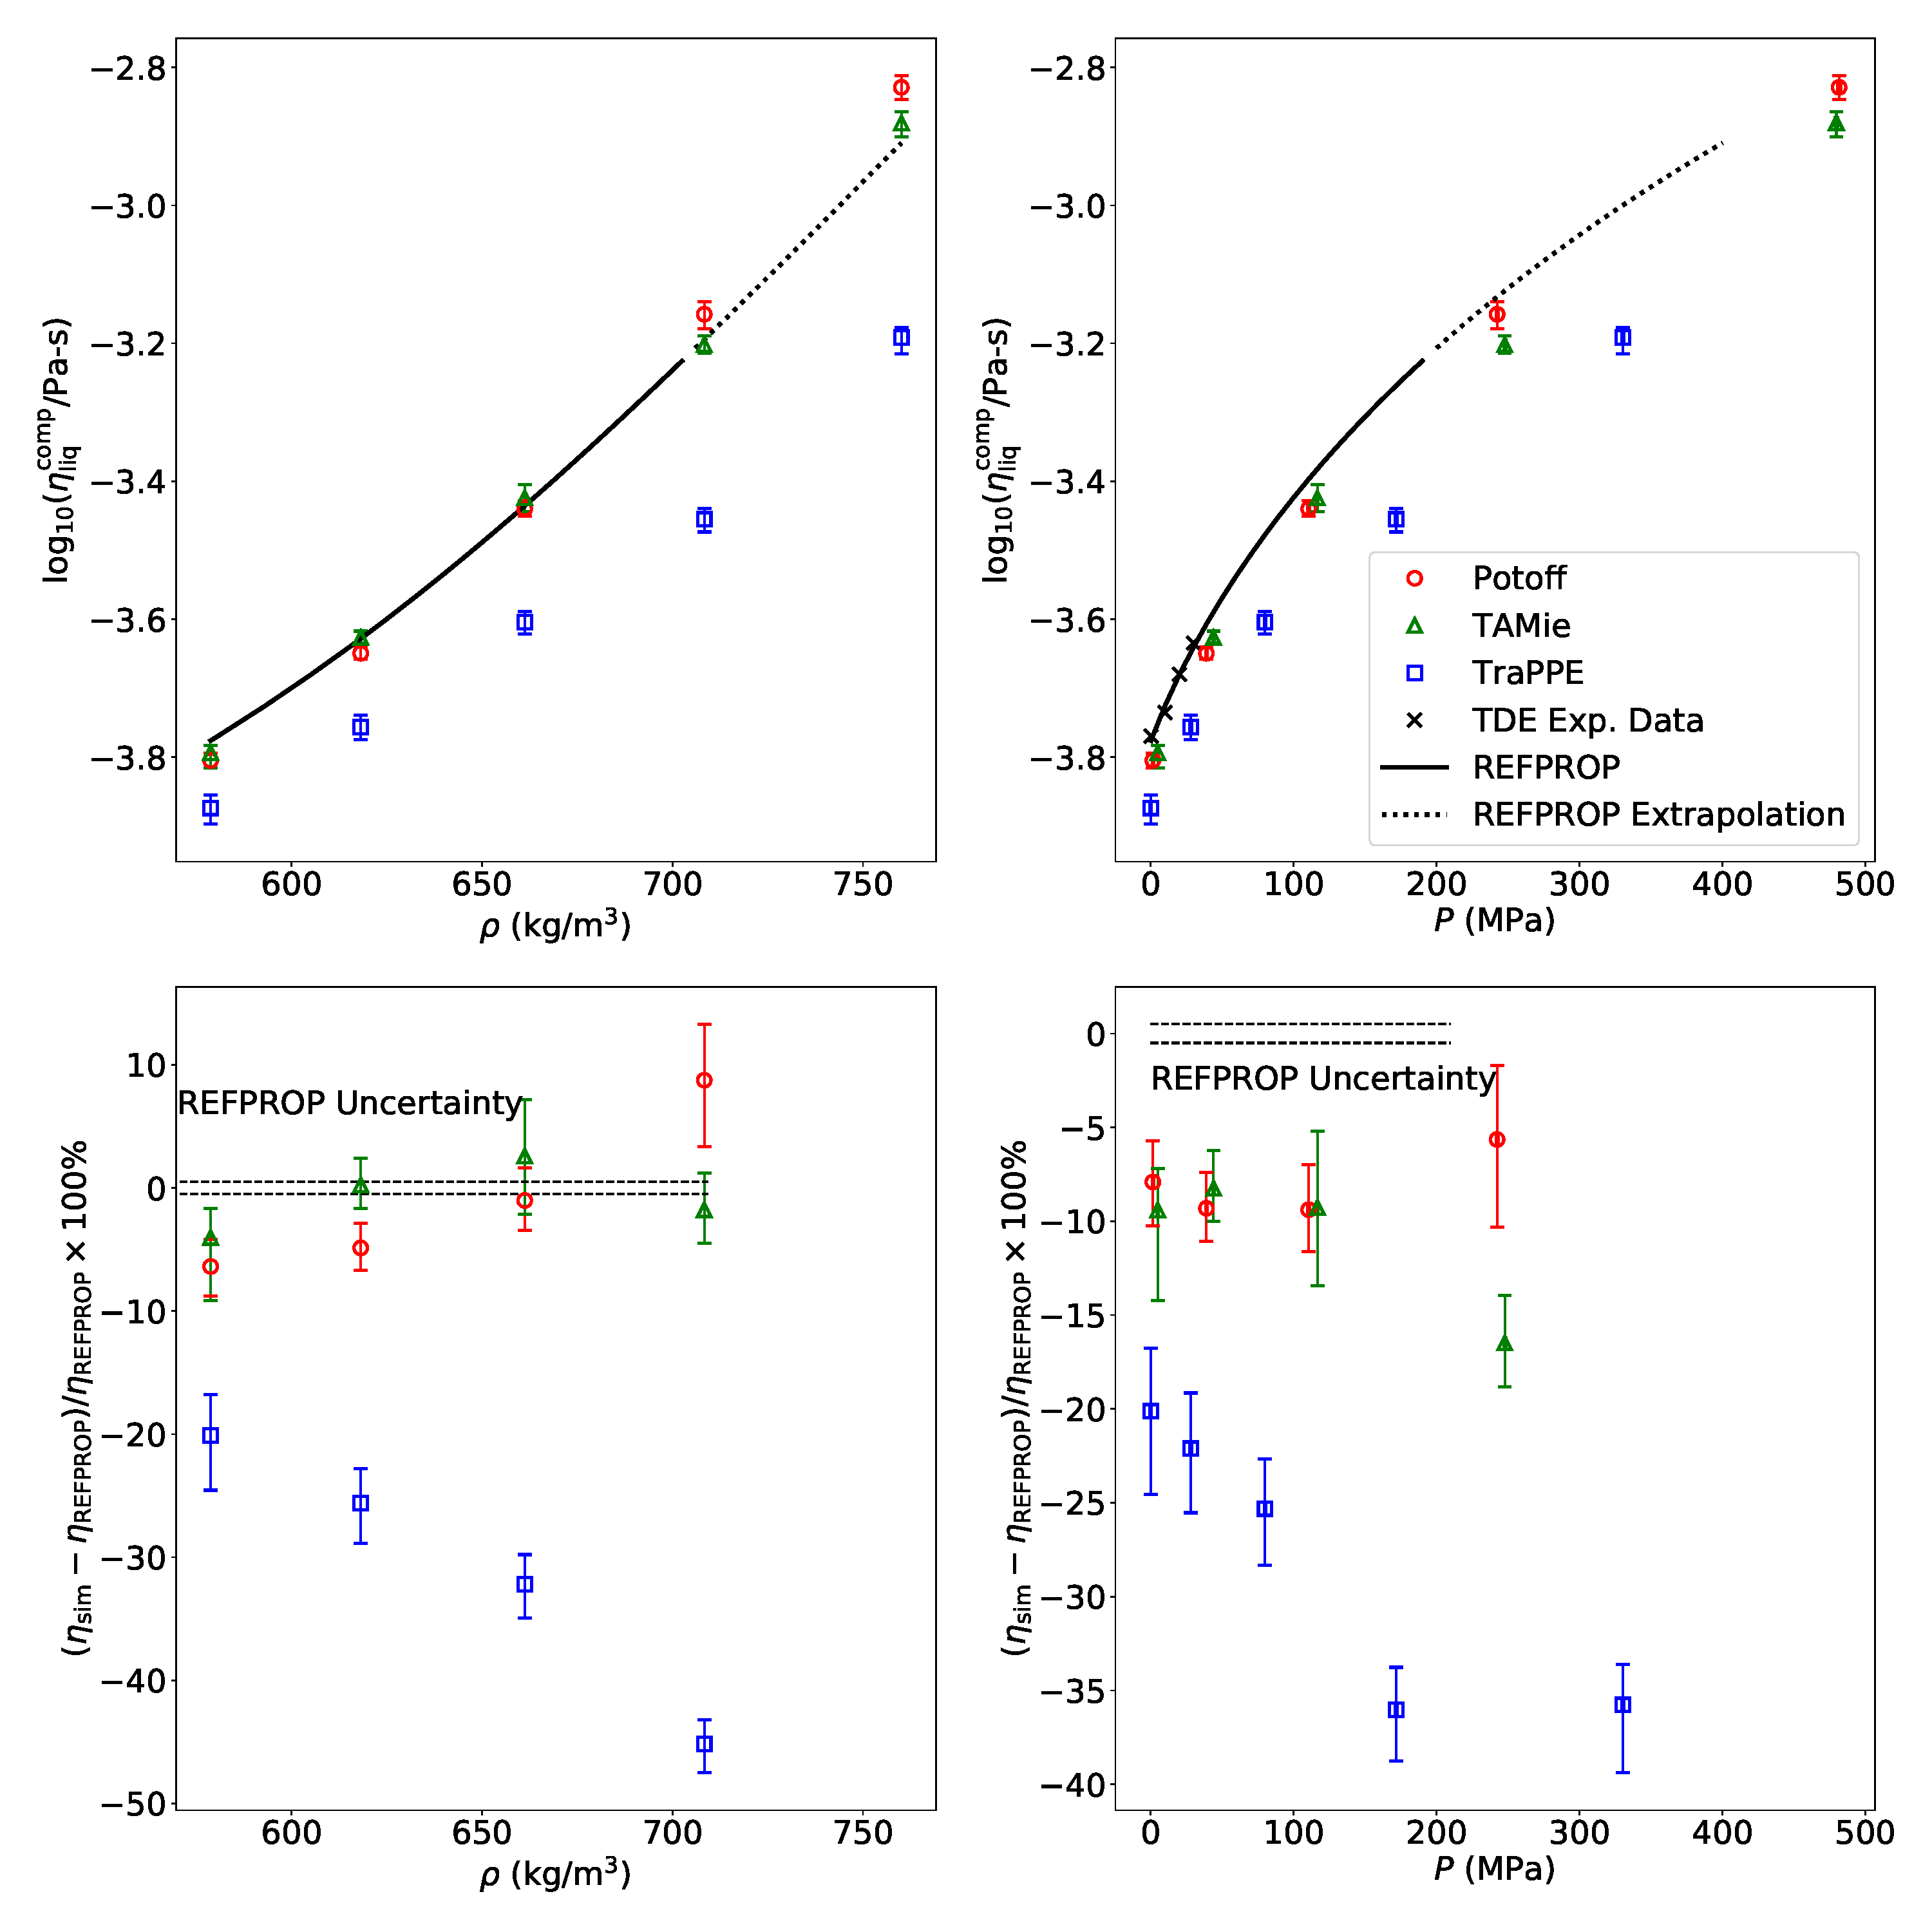
\includegraphics[width=6.4in]{compare_REFPROP_T293highP_C4H10.pdf}
		\caption{Compressed liquid viscosities at 293 K for \textit{n}-butane. See Figure \ref{fig:T293highP_C3} caption for details.}
		\label{fig:T293highP_C4}
	\end{figure} 
	
	\begin{figure}[htb!]
		\centering
		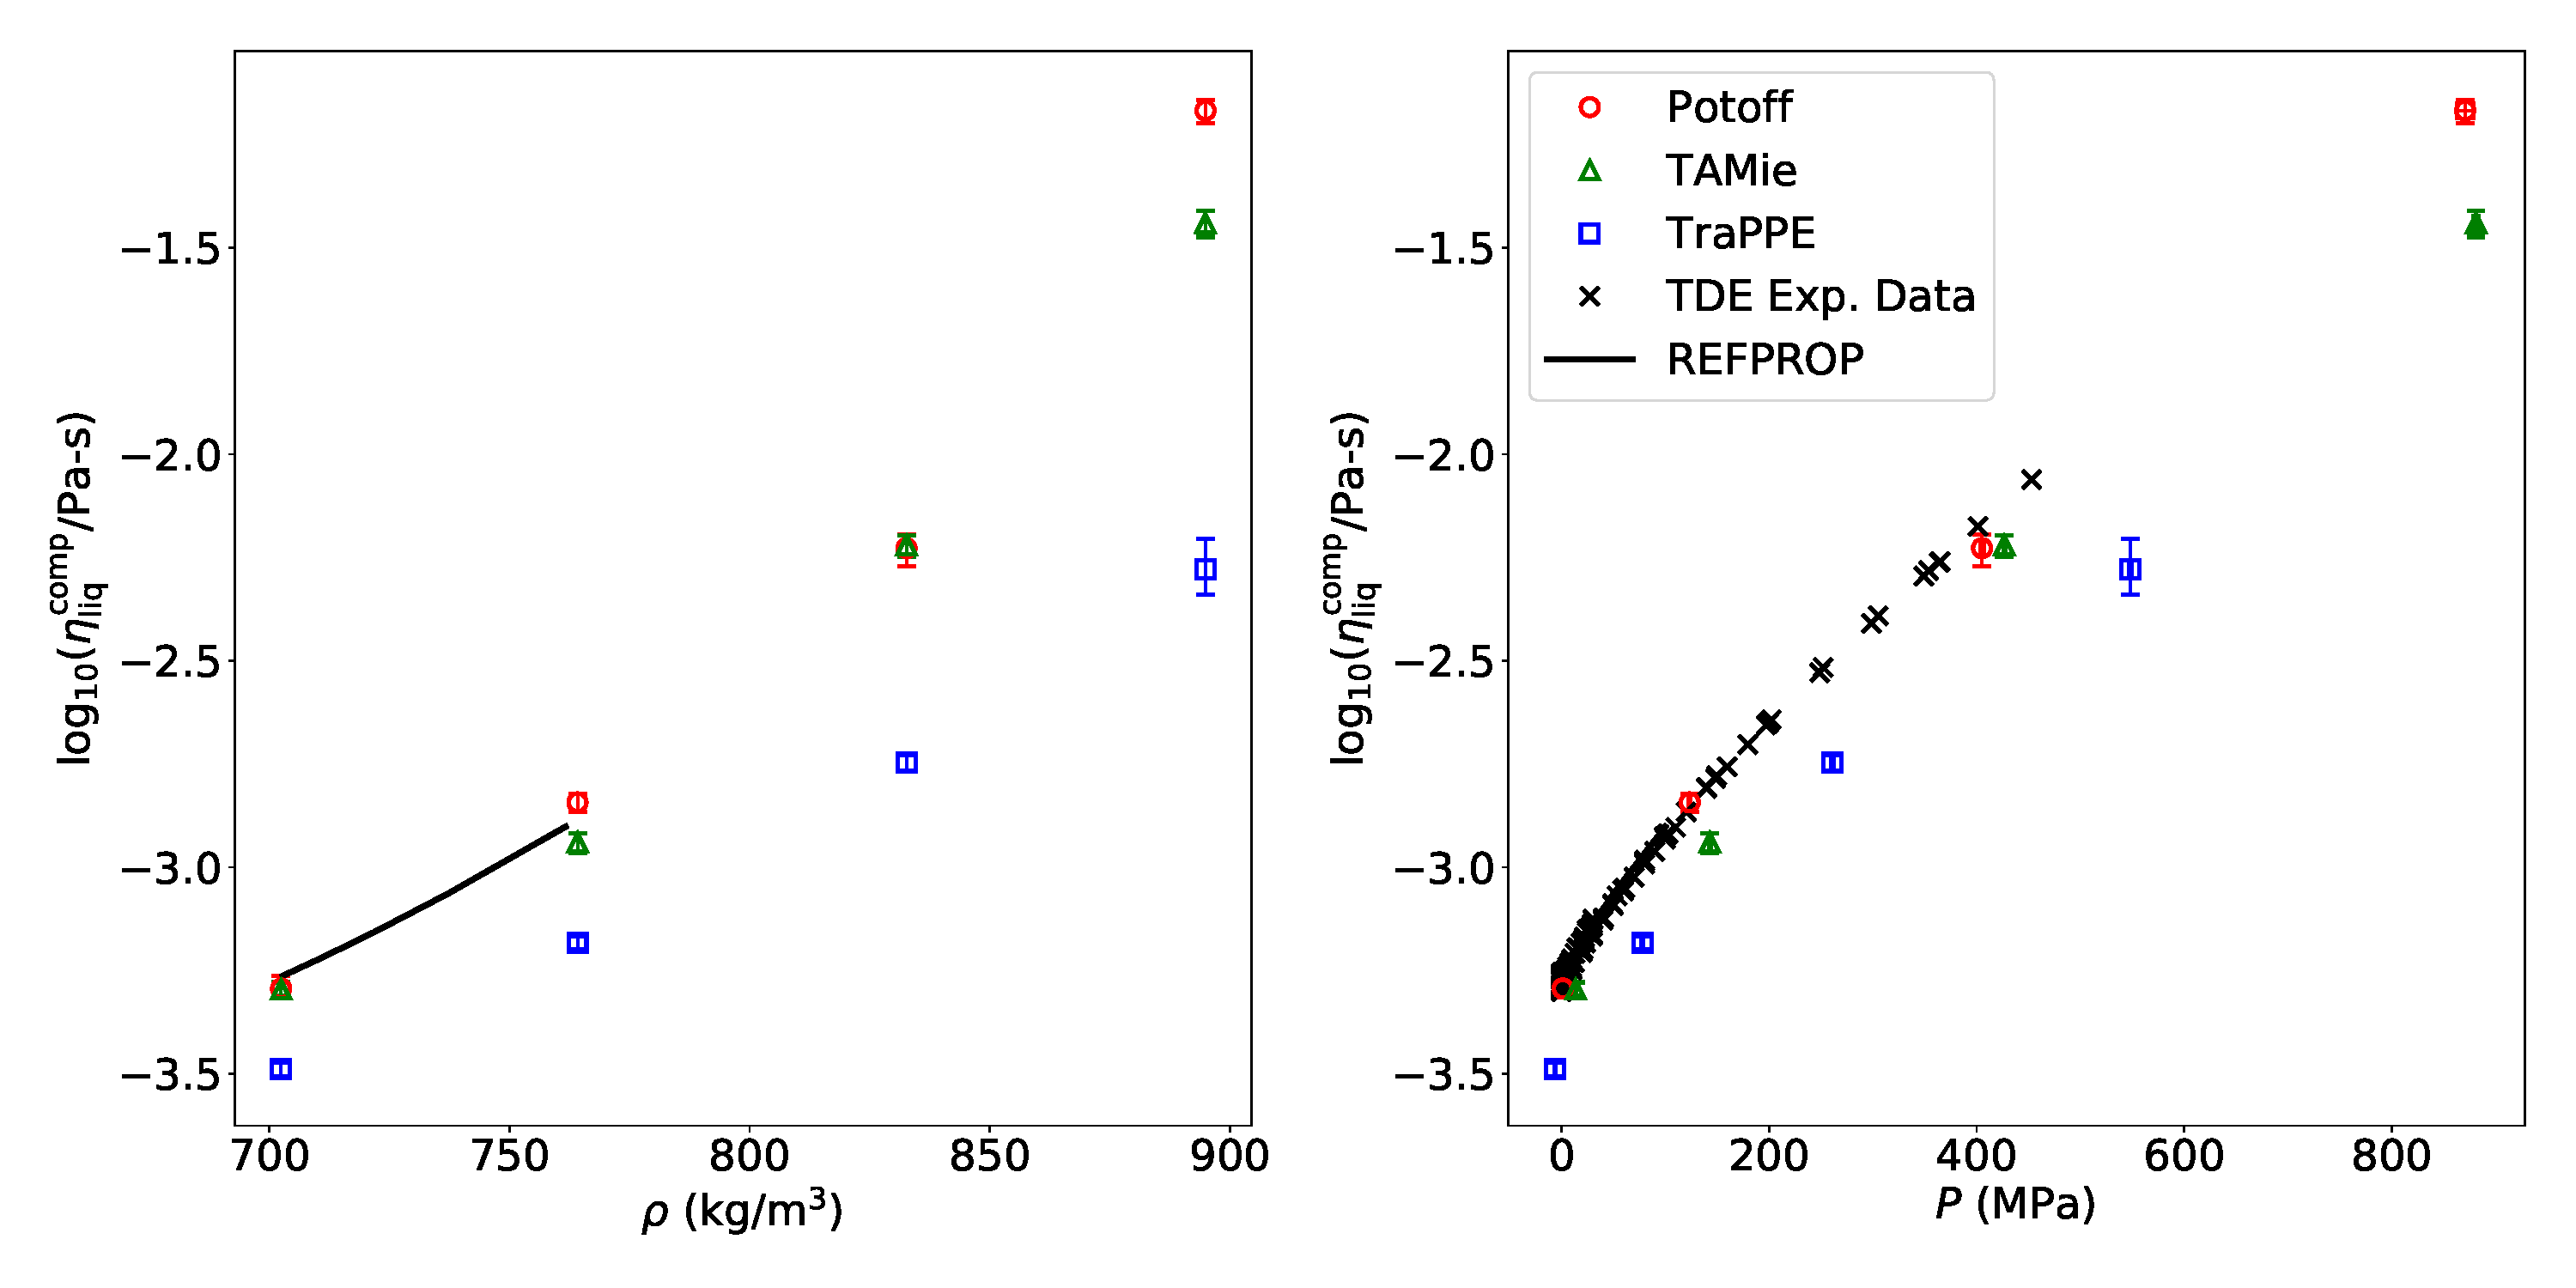
\includegraphics[width=6.4in]{compare_REFPROP_T293highP_C8H18.pdf}
		\caption{Compressed liquid viscosities at 293 K for \textit{n}-octane. See Figure \ref{fig:T293highP_C3} caption for details.}
		\label{fig:T293highP_C8}
	\end{figure} 
	
%	The results in Figures \ref{fig:T293highP_C4} and \ref{fig:T293highP_C8} for \textit{n}-butane and \textit{n}-octane, respectively, are similar to those in Figure \ref{fig:T293highP_C3} for propane. Specifically, the TraPPE force field under estimates $\eta$ at all densities/pressures, the TAMie force field provides the most accurate $\eta$-$\rho$ dependence, while the Potoff force field over predicts $\eta$ with respect to $\rho$ but accurately predicts the $\eta$-$P$ trend. We conclude that Potoff should not be used to estimate the $\eta$-$\rho$ dependence, although it is the most reliable force field for estimating the $\eta$-$P$ dependence.
	
	%, which is often the desired relationship in practice.  
	
	\subsubsection{Branched alkanes}
	
%	\begin{enumerate}
%		\item Similar to n-alkanes? 
%		\item Wrong torsions matters?
%	\end{enumerate}
	
	%Figures:
	%
	%\begin{enumerate}
	%	\item Isobutane $\eta-\rho$ $\eta-P$
	%	\item Isopentane $\eta-\rho$ $\eta-P$
	%	%	\item Isohexane $\eta-\rho$ $\eta-P$?
	%	\item Isooctane $\eta-\rho$ $\eta-P$
	%	%	\item Neopentane $\eta-\rho$ $\eta-P$?
	%	\item 3-methylpentane $\eta-\rho$ $\eta-P$?
	%	%	\item 2,3-dimethylbutane $\eta-\rho$ $\eta-P$?
	%\end{enumerate}
	
   The trends observed in Figures \ref{fig:T293highP_IC4} to \ref{fig:T293highP_IC8} are consistent with the compressed liquid trends for \textit{n}-alkanes. Specifically, TraPPE under predicts $\eta$ with respect to both $\rho$ and $P$. Potoff over predicts $\eta$ with respect to $\rho$ but provides a reasonable estimate of the $\eta$-$P$ trend. However, as observed in Section \ref{sec:eta_sat}, Potoff and TAMie are less accurate for branched alkanes than for \textit{n}-alkanes. In particular, the Potoff $\eta$-$P$ trends are systematically lower than the REFPROP correlations for 2-methylbutane and 3-methylpentane. However, note that the Potoff $\eta$-$P$ trends are quite reliable for 2-methylpropane and 2,2,4-trimethylpentane. These results cannot be attributed to the ``short'' or ``long'' parameter distinction, since 2-methylbutane and 2-methylpropane both use ``short'' parameters while 3-methylpentane and 2,2,4-trimethylpentane both use ``long'' parameters. 
	
	\begin{figure}[htb!]
		\centering
		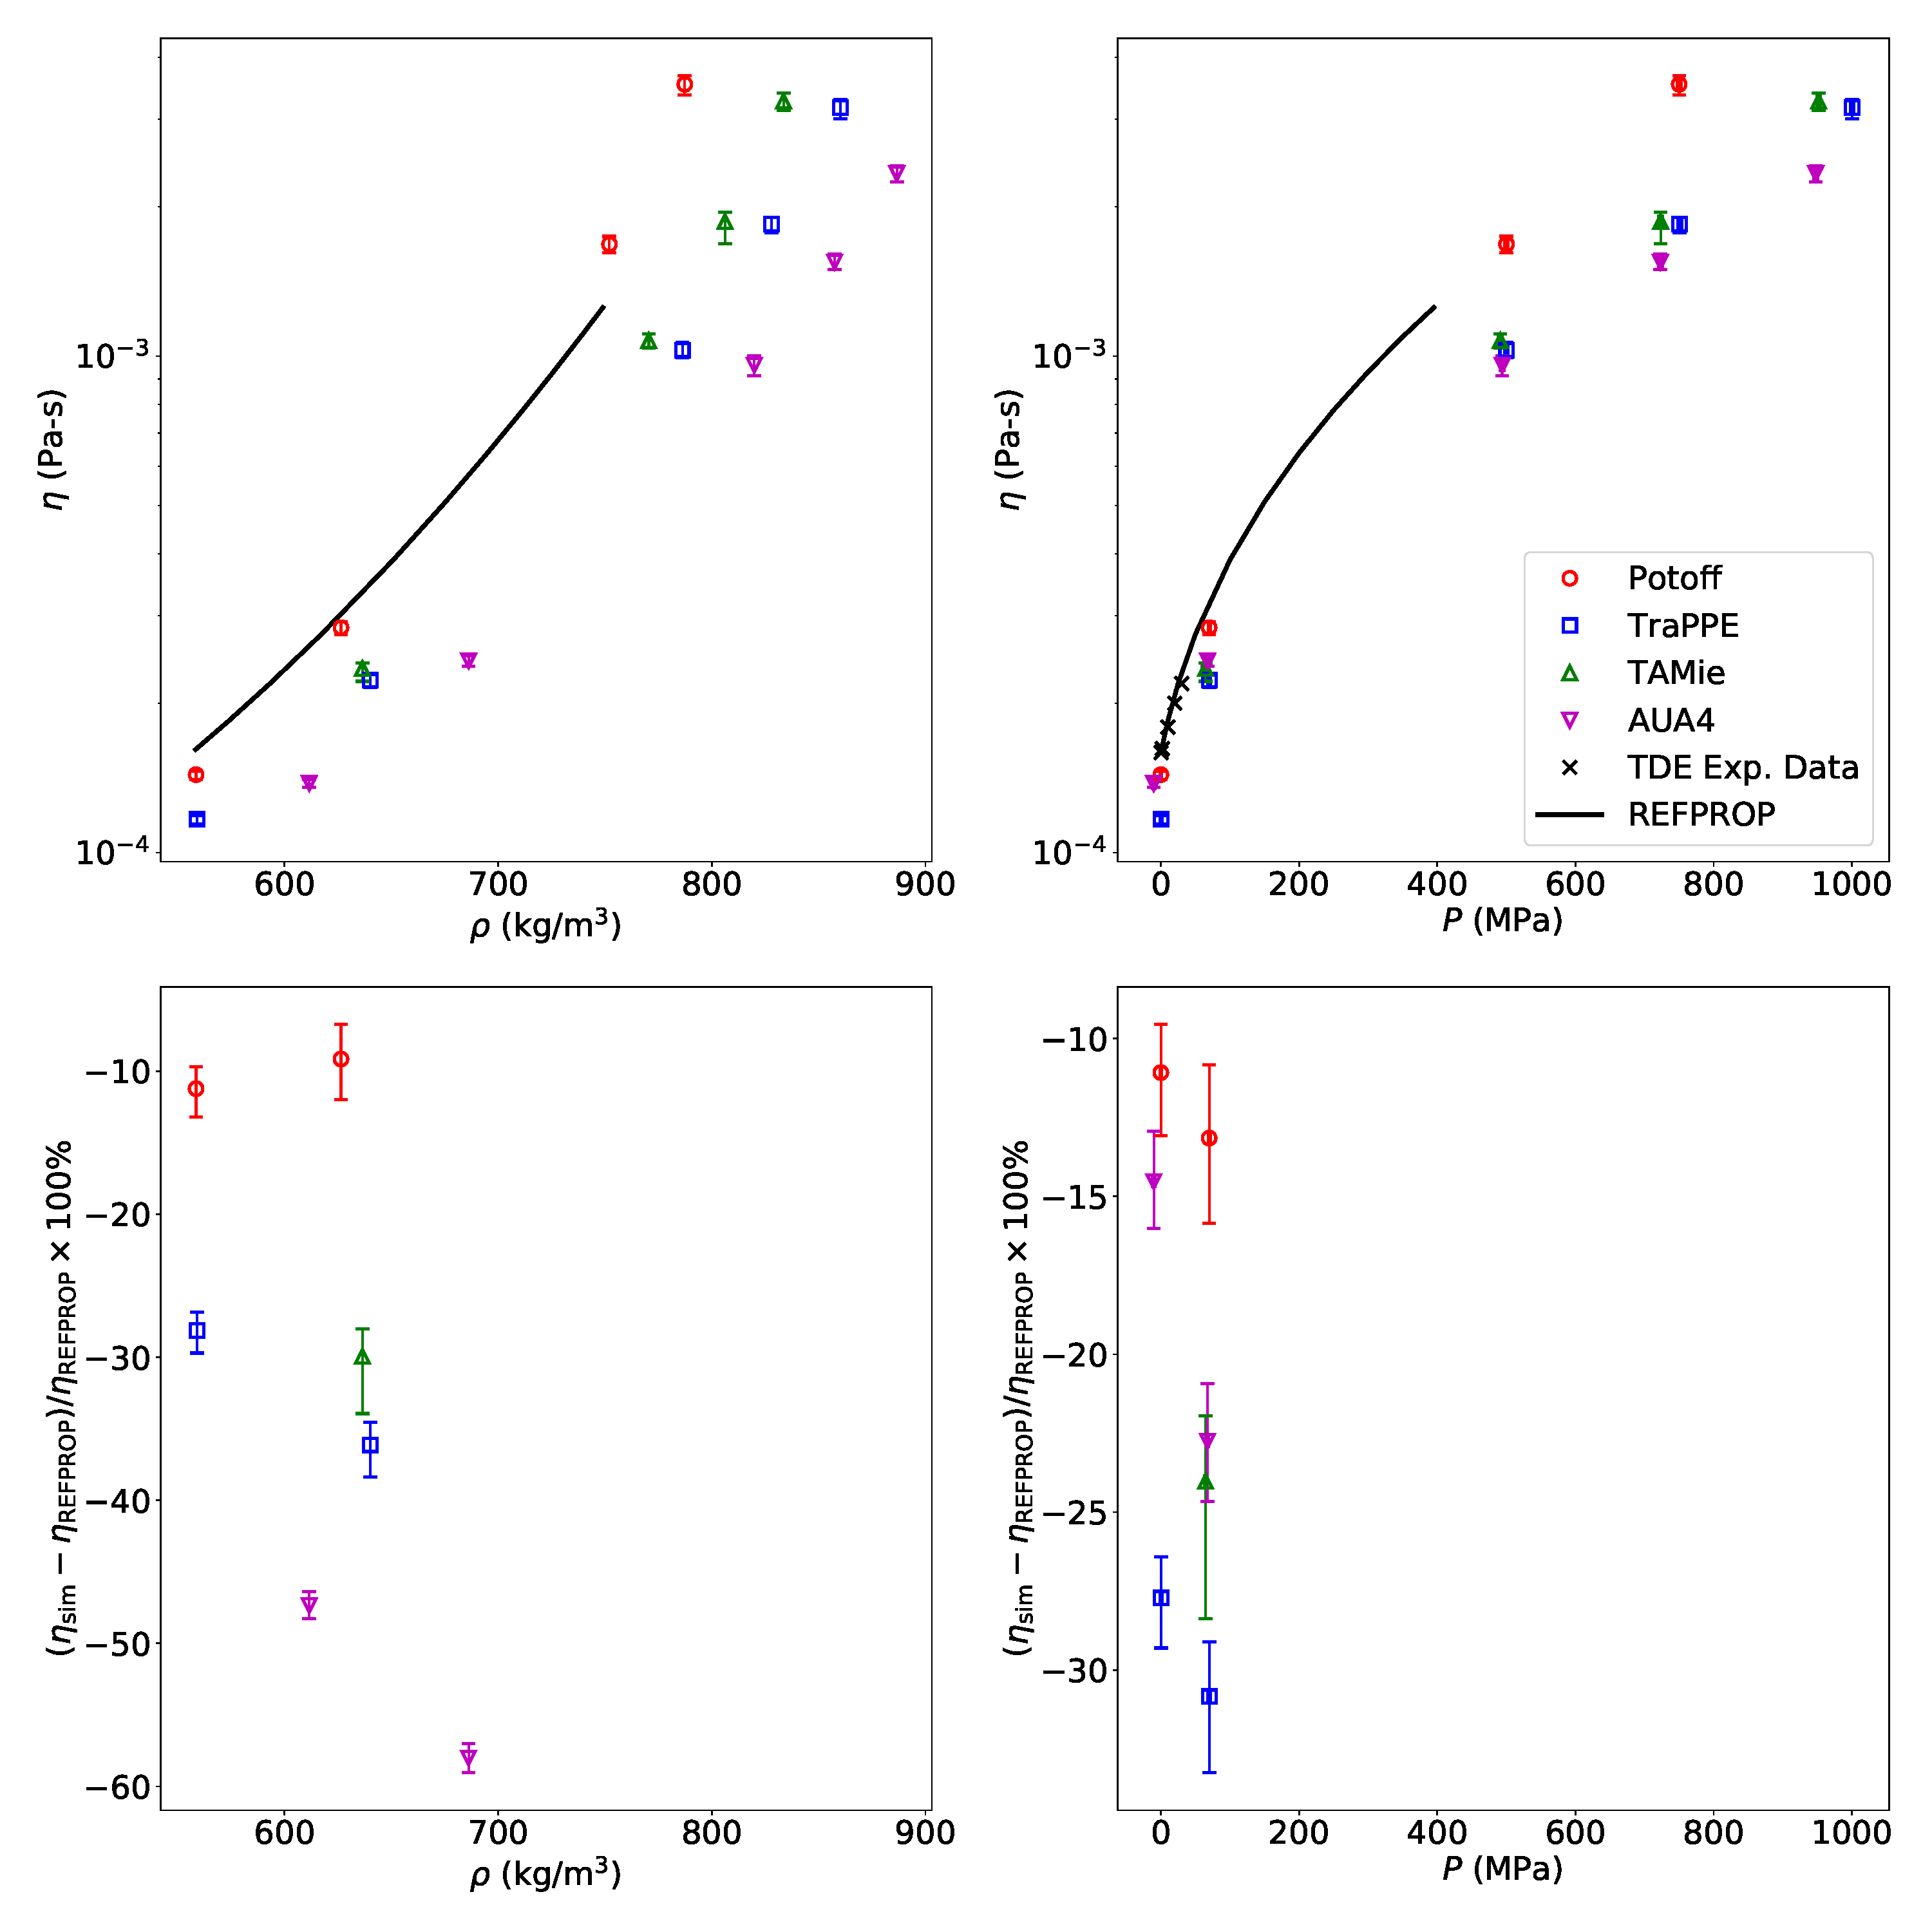
\includegraphics[width=6.4in]{compare_REFPROP_T293highP_IC4H10.pdf}
		\caption{Compressed liquid viscosities at 293 K for 2-methylpropane. See Figure \ref{fig:T293highP_C3} caption for details.}
		\label{fig:T293highP_IC4}
	\end{figure} 
	
	\begin{figure}[htb!]
		\centering
		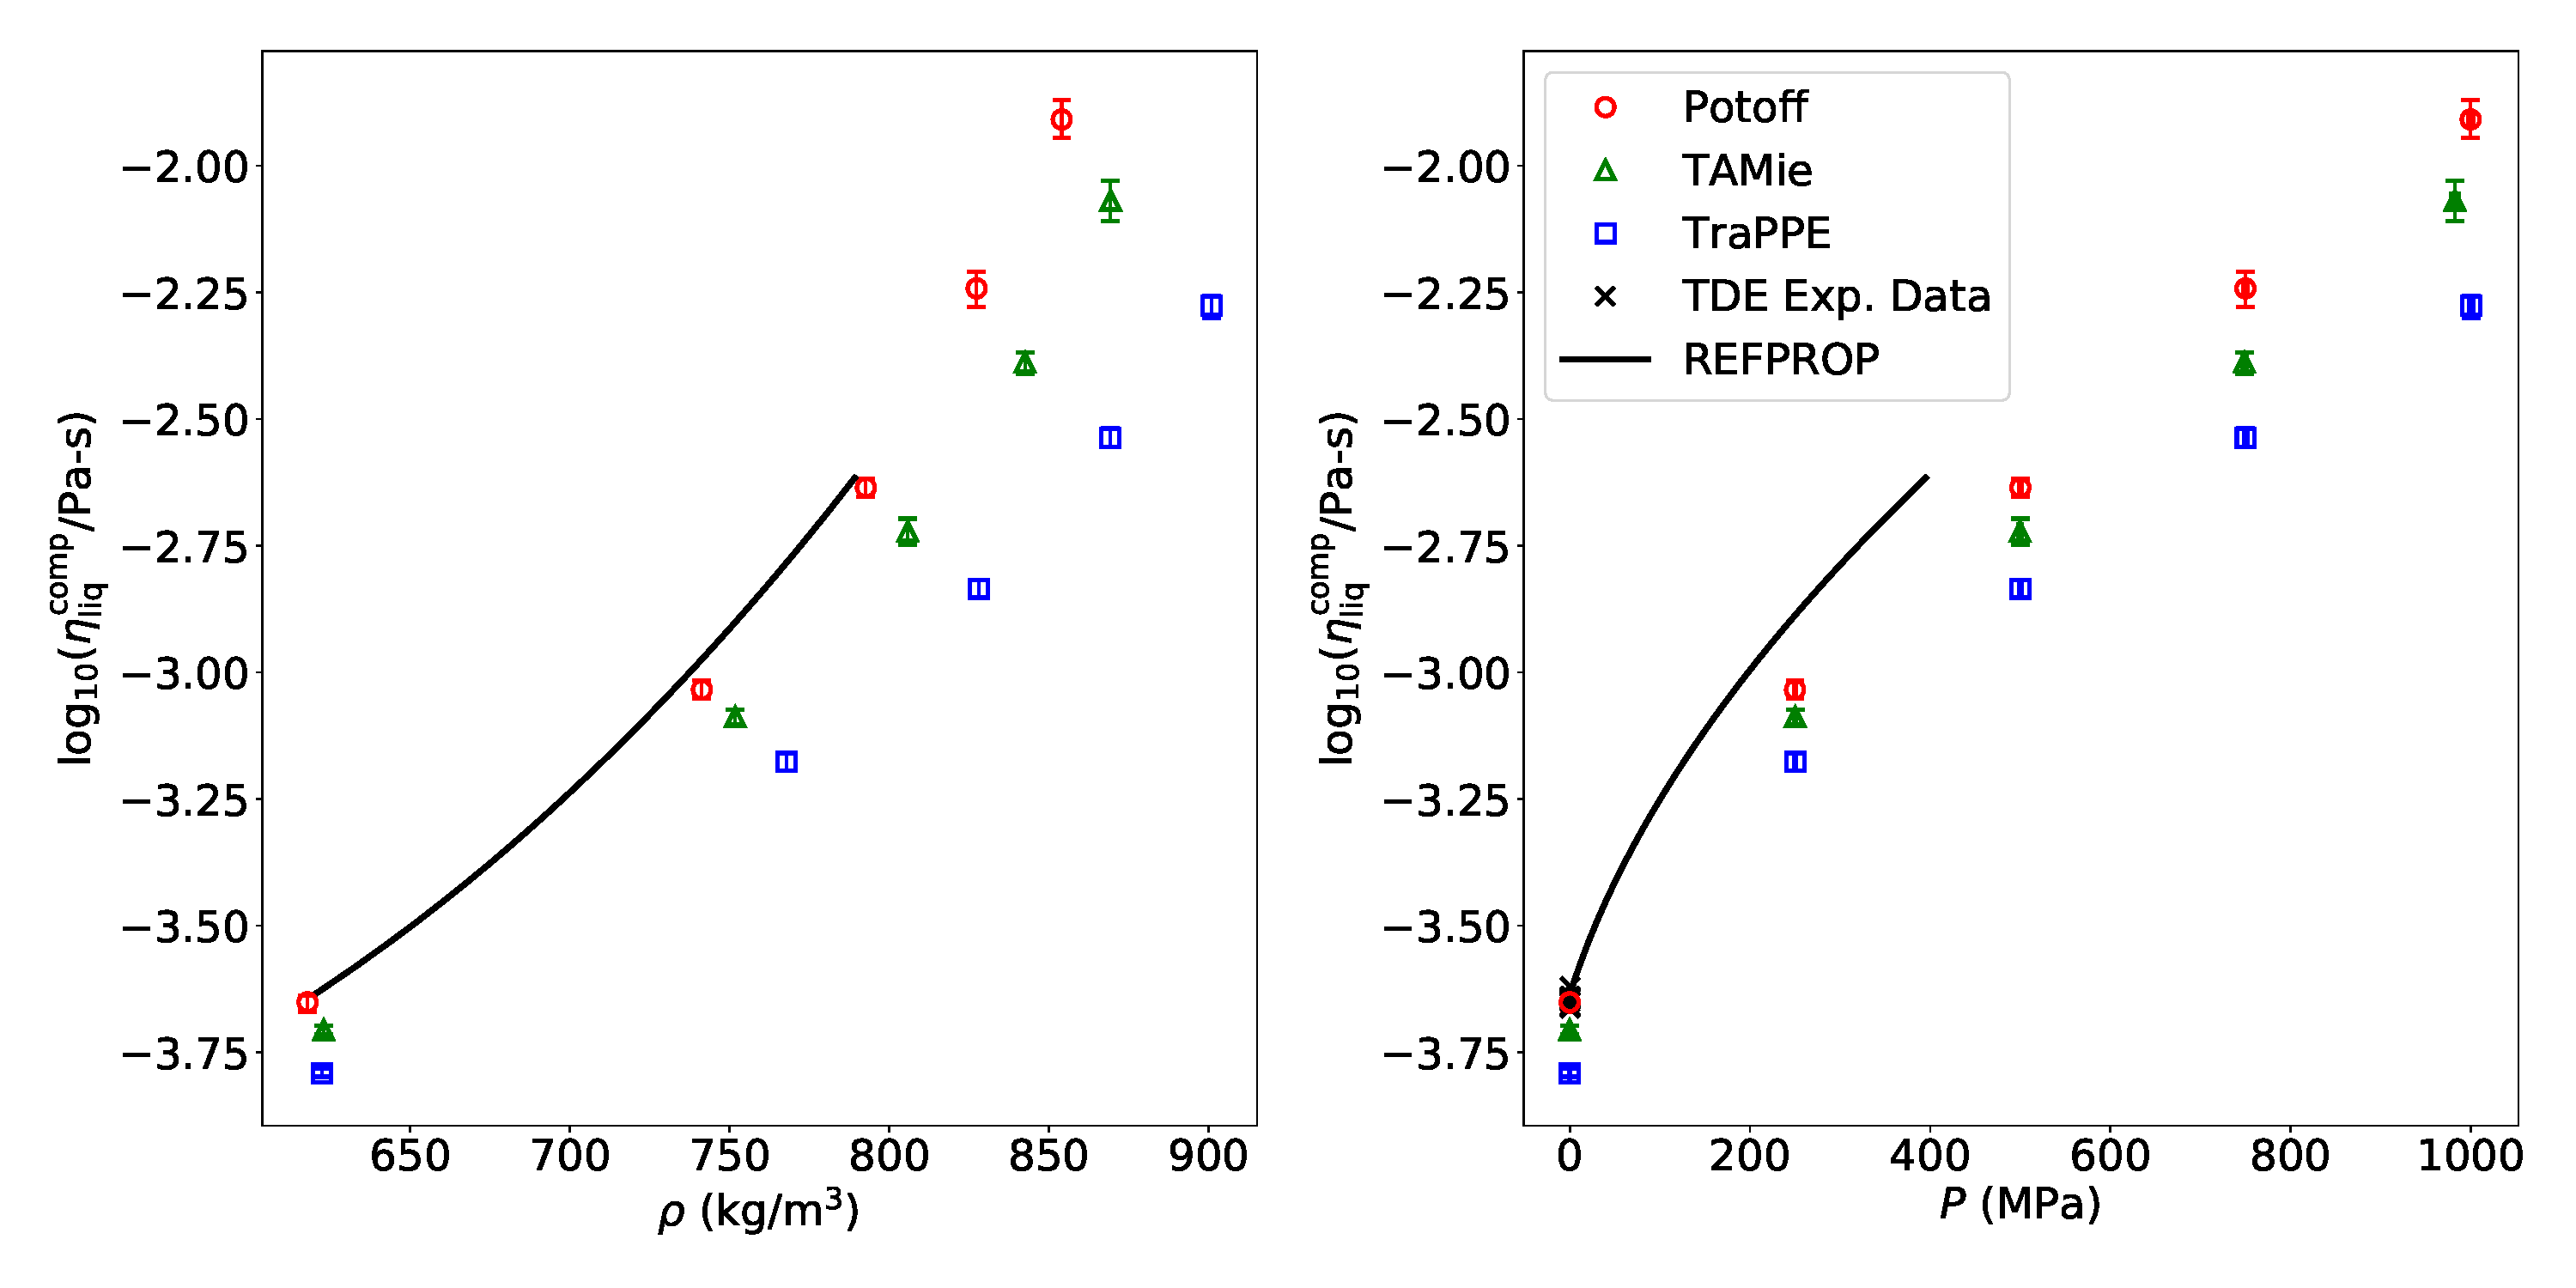
\includegraphics[width=6.4in]{compare_REFPROP_T293highP_IC5H12.pdf}
		\caption{Compressed liquid viscosities at 293 K for 2-methylbutane. See Figure \ref{fig:T293highP_C3} caption for details.}
		\label{fig:T293highP_IC5}
	\end{figure} 
	
	\begin{figure}[htb!]
		\centering
		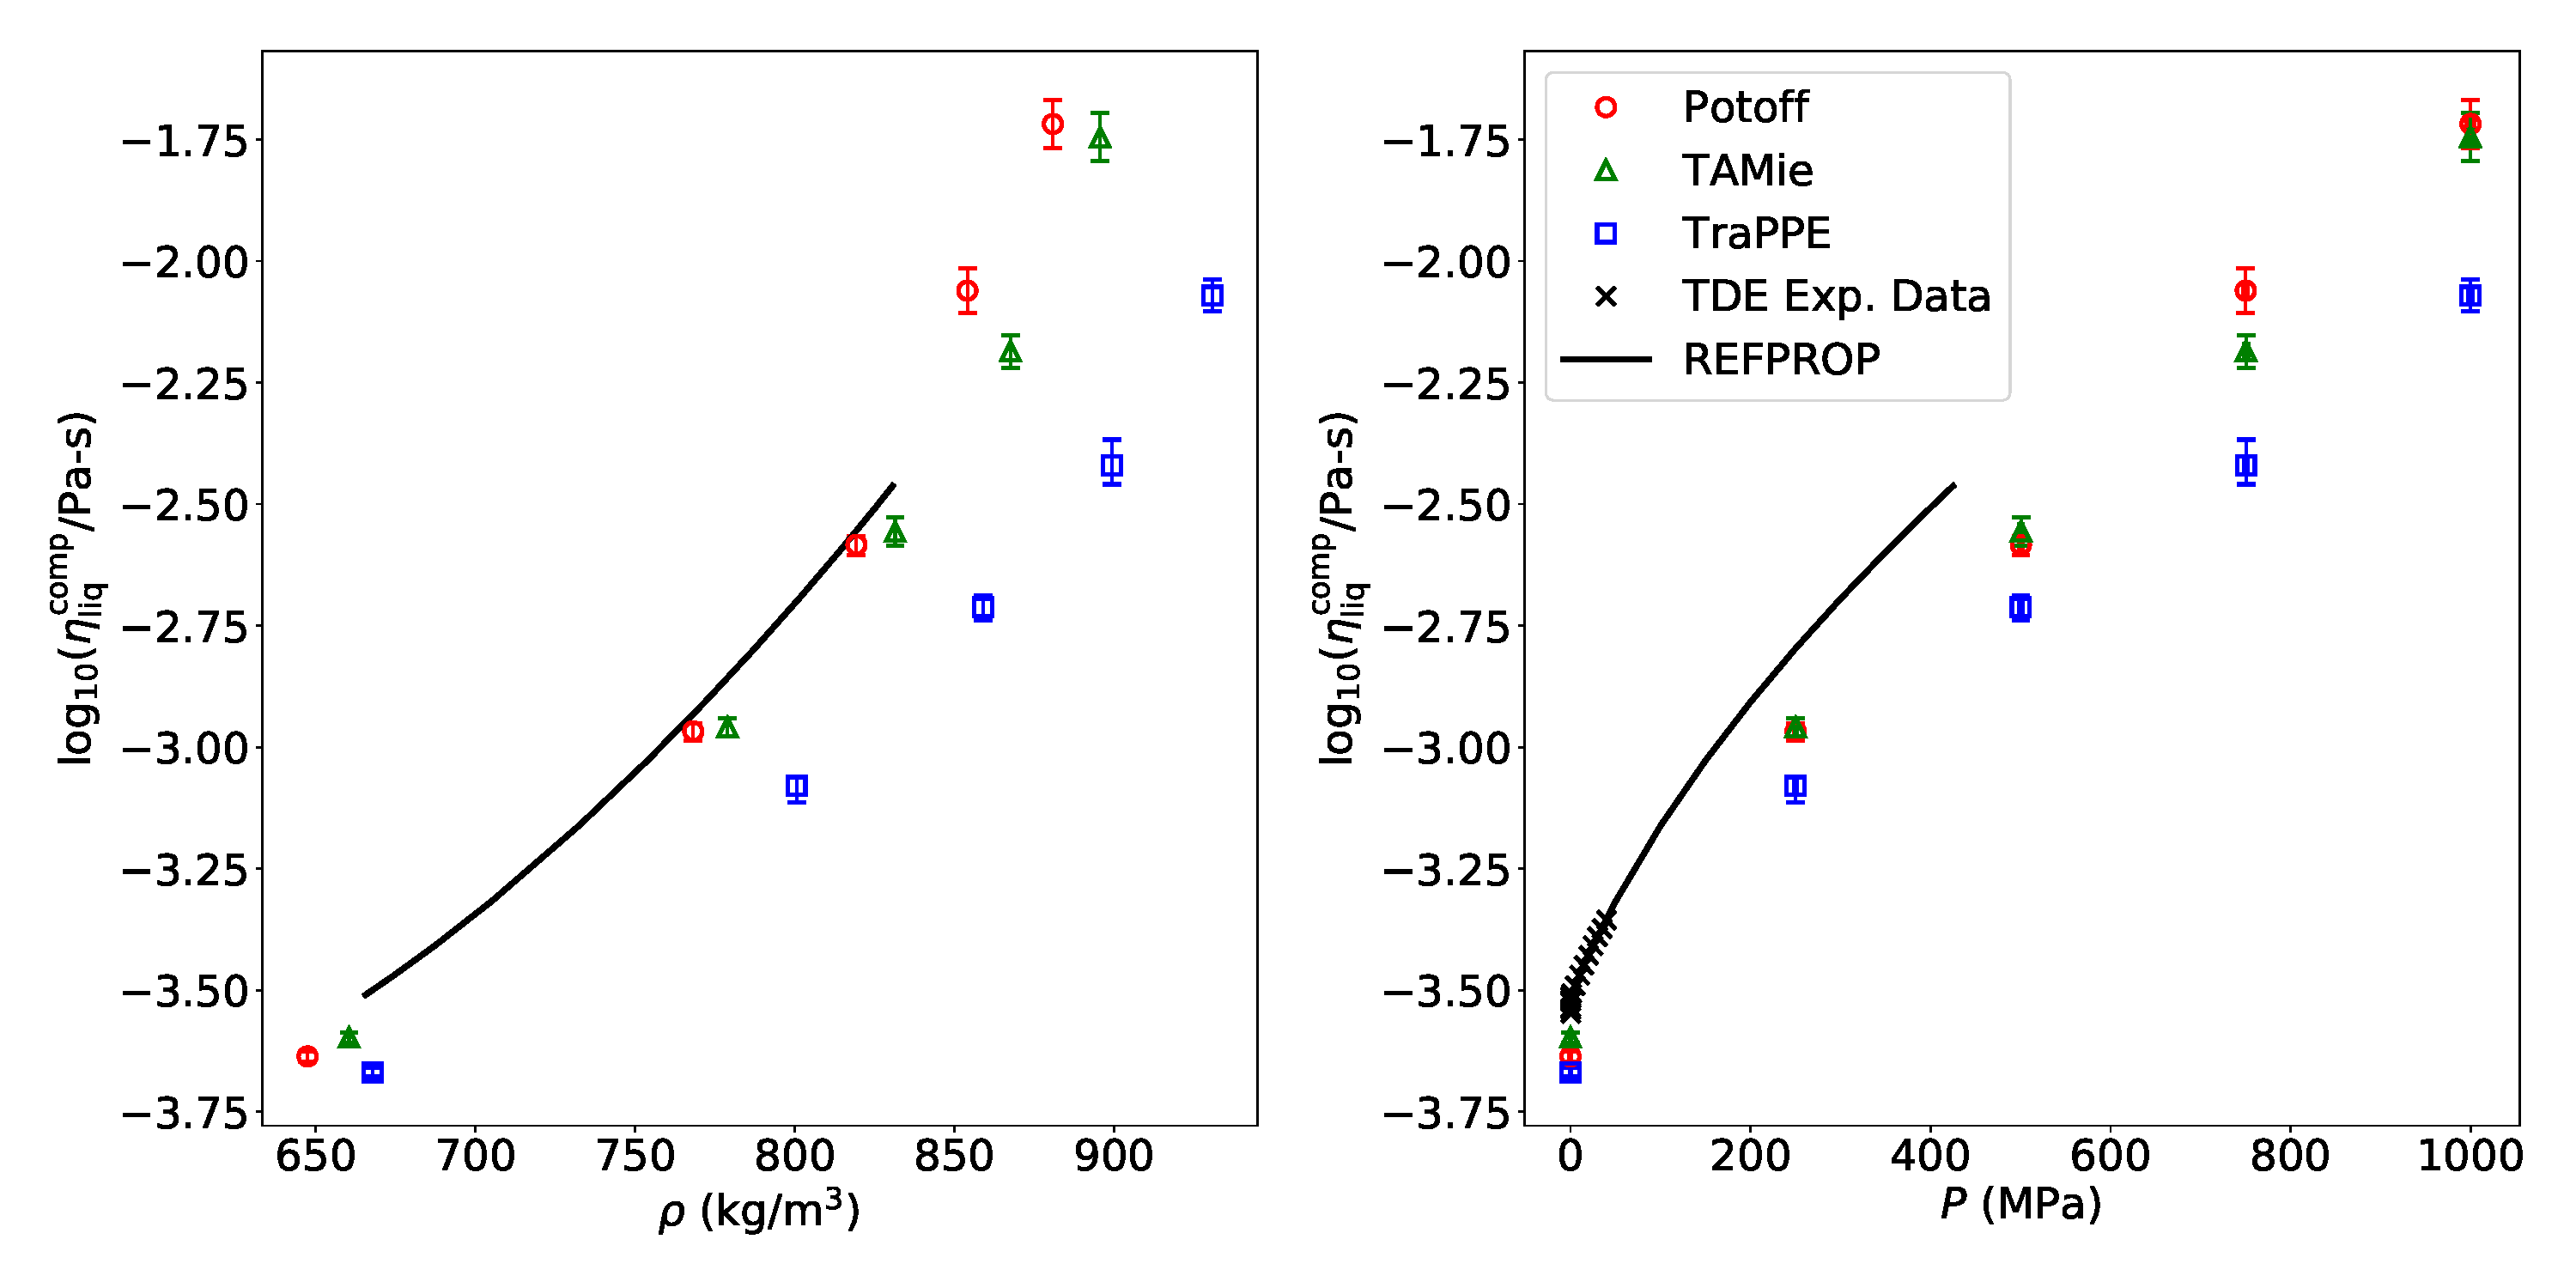
\includegraphics[width=6.4in]{compare_REFPROP_T293highP_3MPentane.pdf}
		\caption{Compressed liquid viscosities at 293 K for 3-methylpentane. See Figure \ref{fig:T293highP_C3} caption for details.}
		\label{fig:T293highP_3MP}
	\end{figure} 
	
	\begin{figure}[htb!]
		\centering
		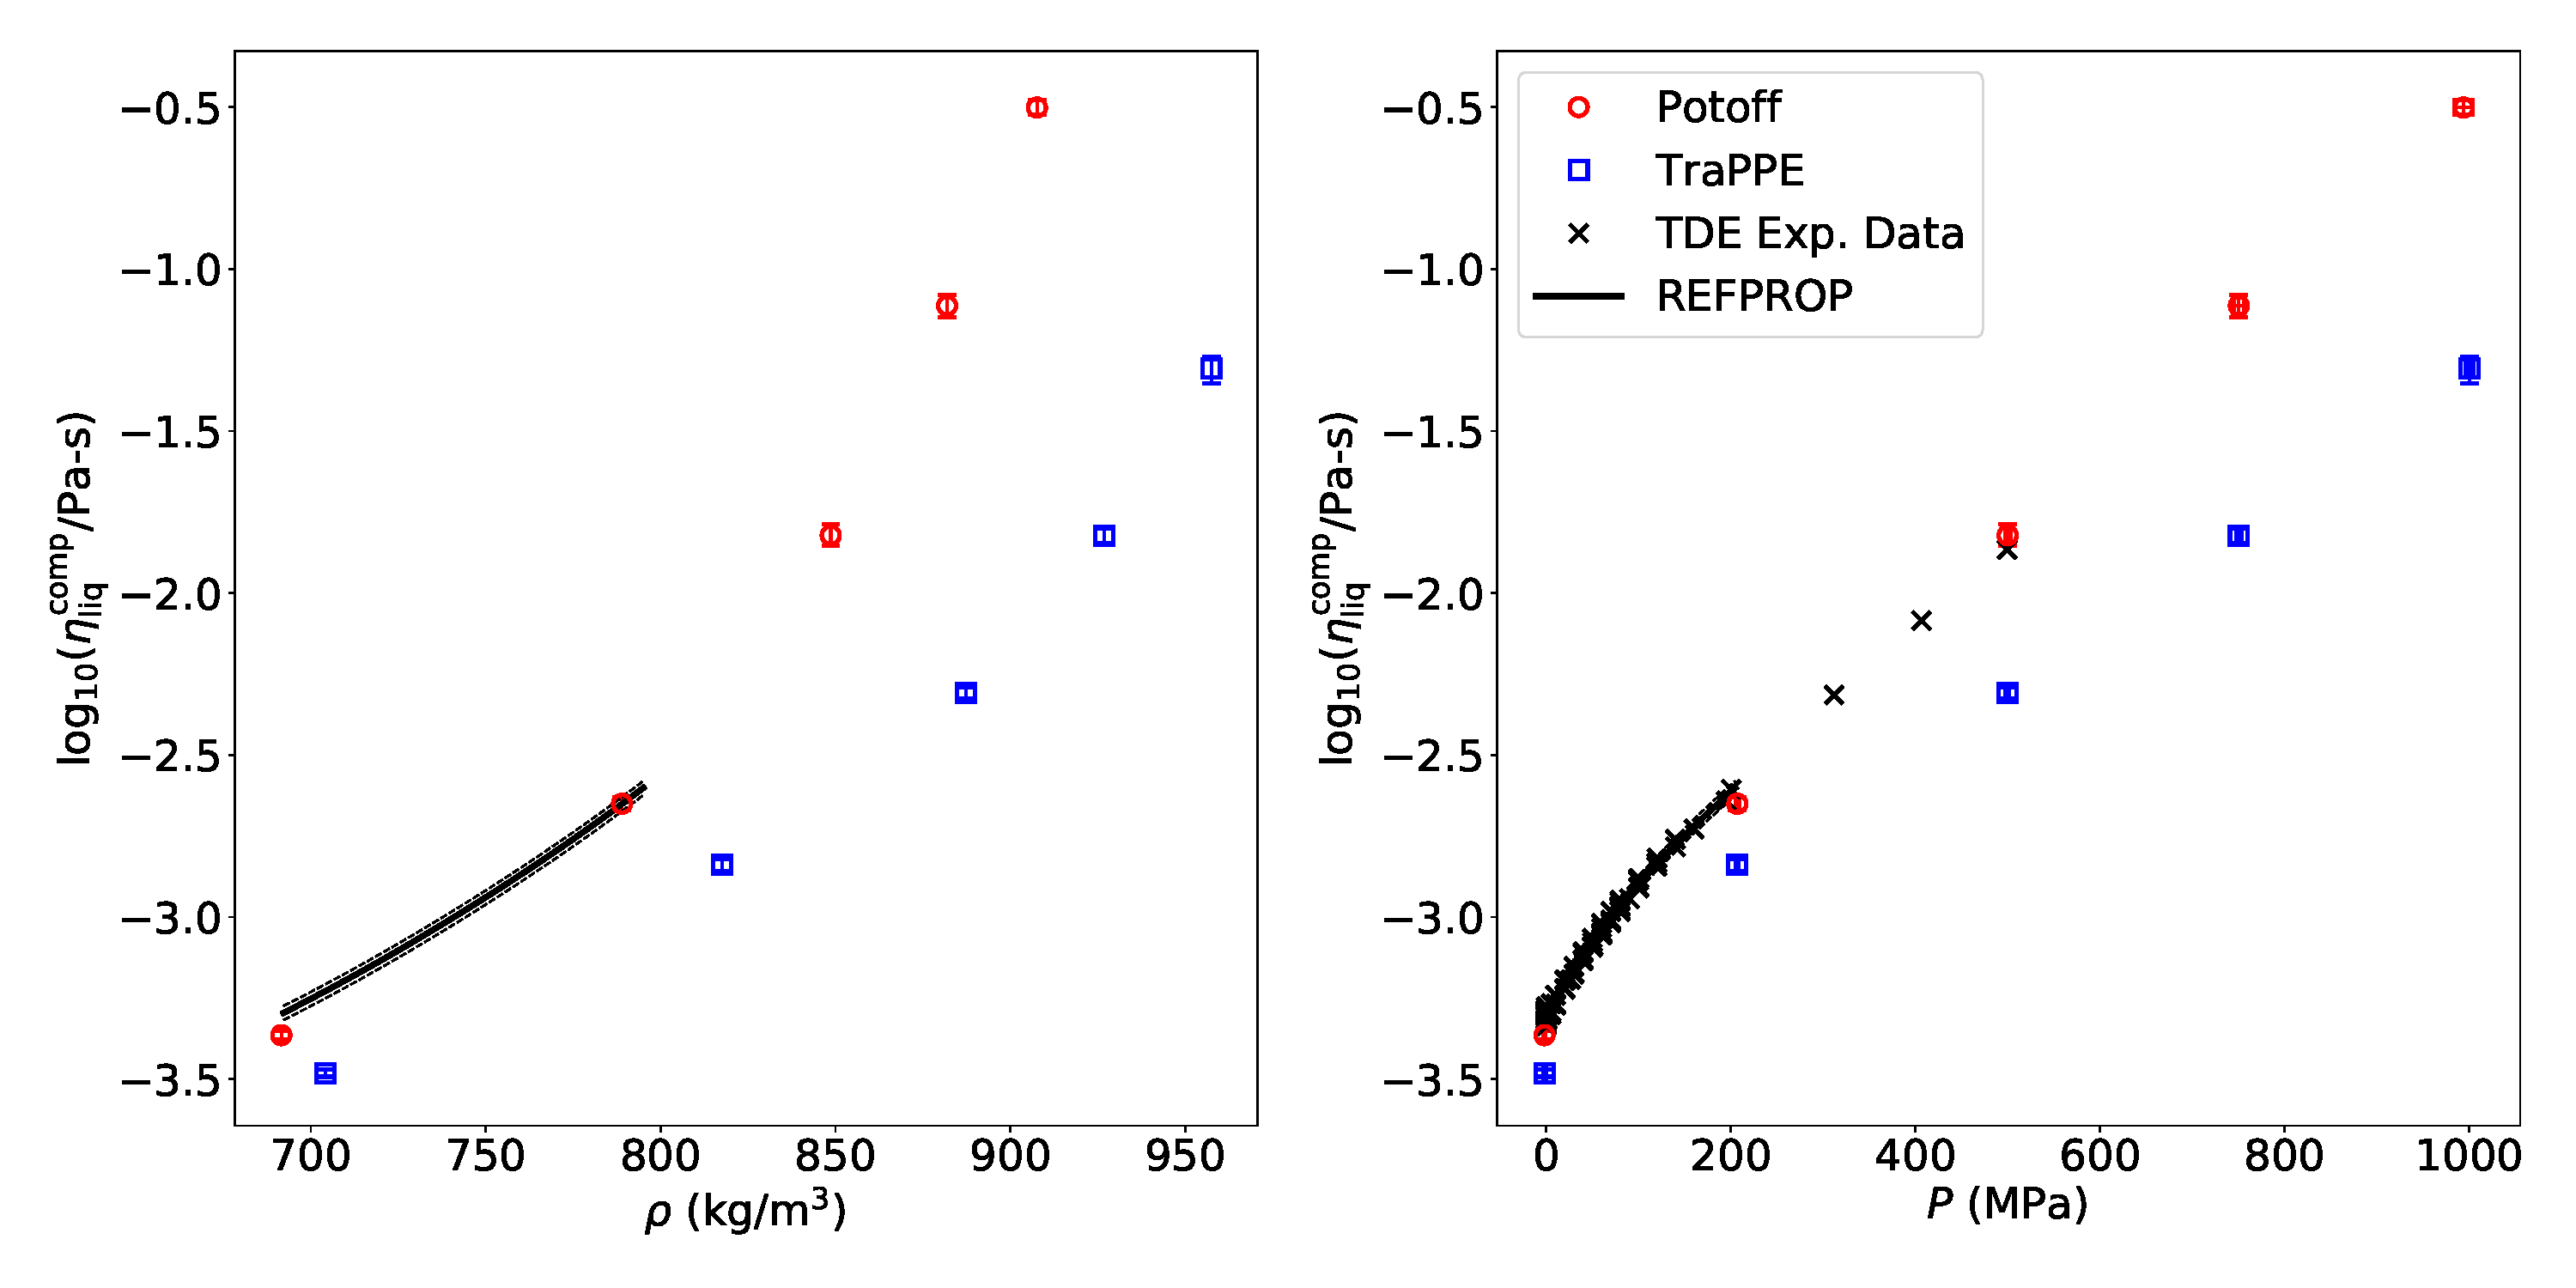
\includegraphics[width=6.4in]{compare_REFPROP_T293highP_IC8H18.pdf}
		\caption{Compressed liquid viscosities at 293 K for 2,2,4-trimethylpentane. See Figure \ref{fig:T293highP_C3} caption for details.}
		\label{fig:T293highP_IC8}
	\end{figure} 
	
	\section{Discussion/Limitations} \label{Discussion/Limitations}
	
	\subsection{Liquid structure} \label{sec:RDF}
	
	While the Potoff force field significantly over predicts the $\eta$-$\rho$ dependence at $T= 293$ K, it does not over predict $\eta$ for the highest saturated liquid densities (those near the triple point temperature) (cf. Figures \ref{fig:Saturation_C3_C4_C8} and \ref{fig:T293highP_C3} for propane). To better understand this seemingly inconsistent result, Figure \ref{fig:RDF_comparison_CH3} compares the radial distribution functions (RDF) for three different state points, namely, near the triple point $(T=86$ K and $\rho = 732.63$ kg/m$^3)$ and two densities along the $T = 293$ K isotherm ($\rho = 732.63$ kg/m$^3$ and $\rho = 806.23$ kg/m$^3)$. In order to provide a fair comparison between force fields, the RDF is plotted with respect to a reduced distance, namely, $r/r_{\rm min}$.
	
	% $(T_{\rm tp}$ and $\rho_{\rm tp})$ and two densities along the $T = 293$ K isotherm ($\rho_{\rm tp}$ and the maximum $\rho$)
	
	\begin{figure}[htb!]
		\centering
		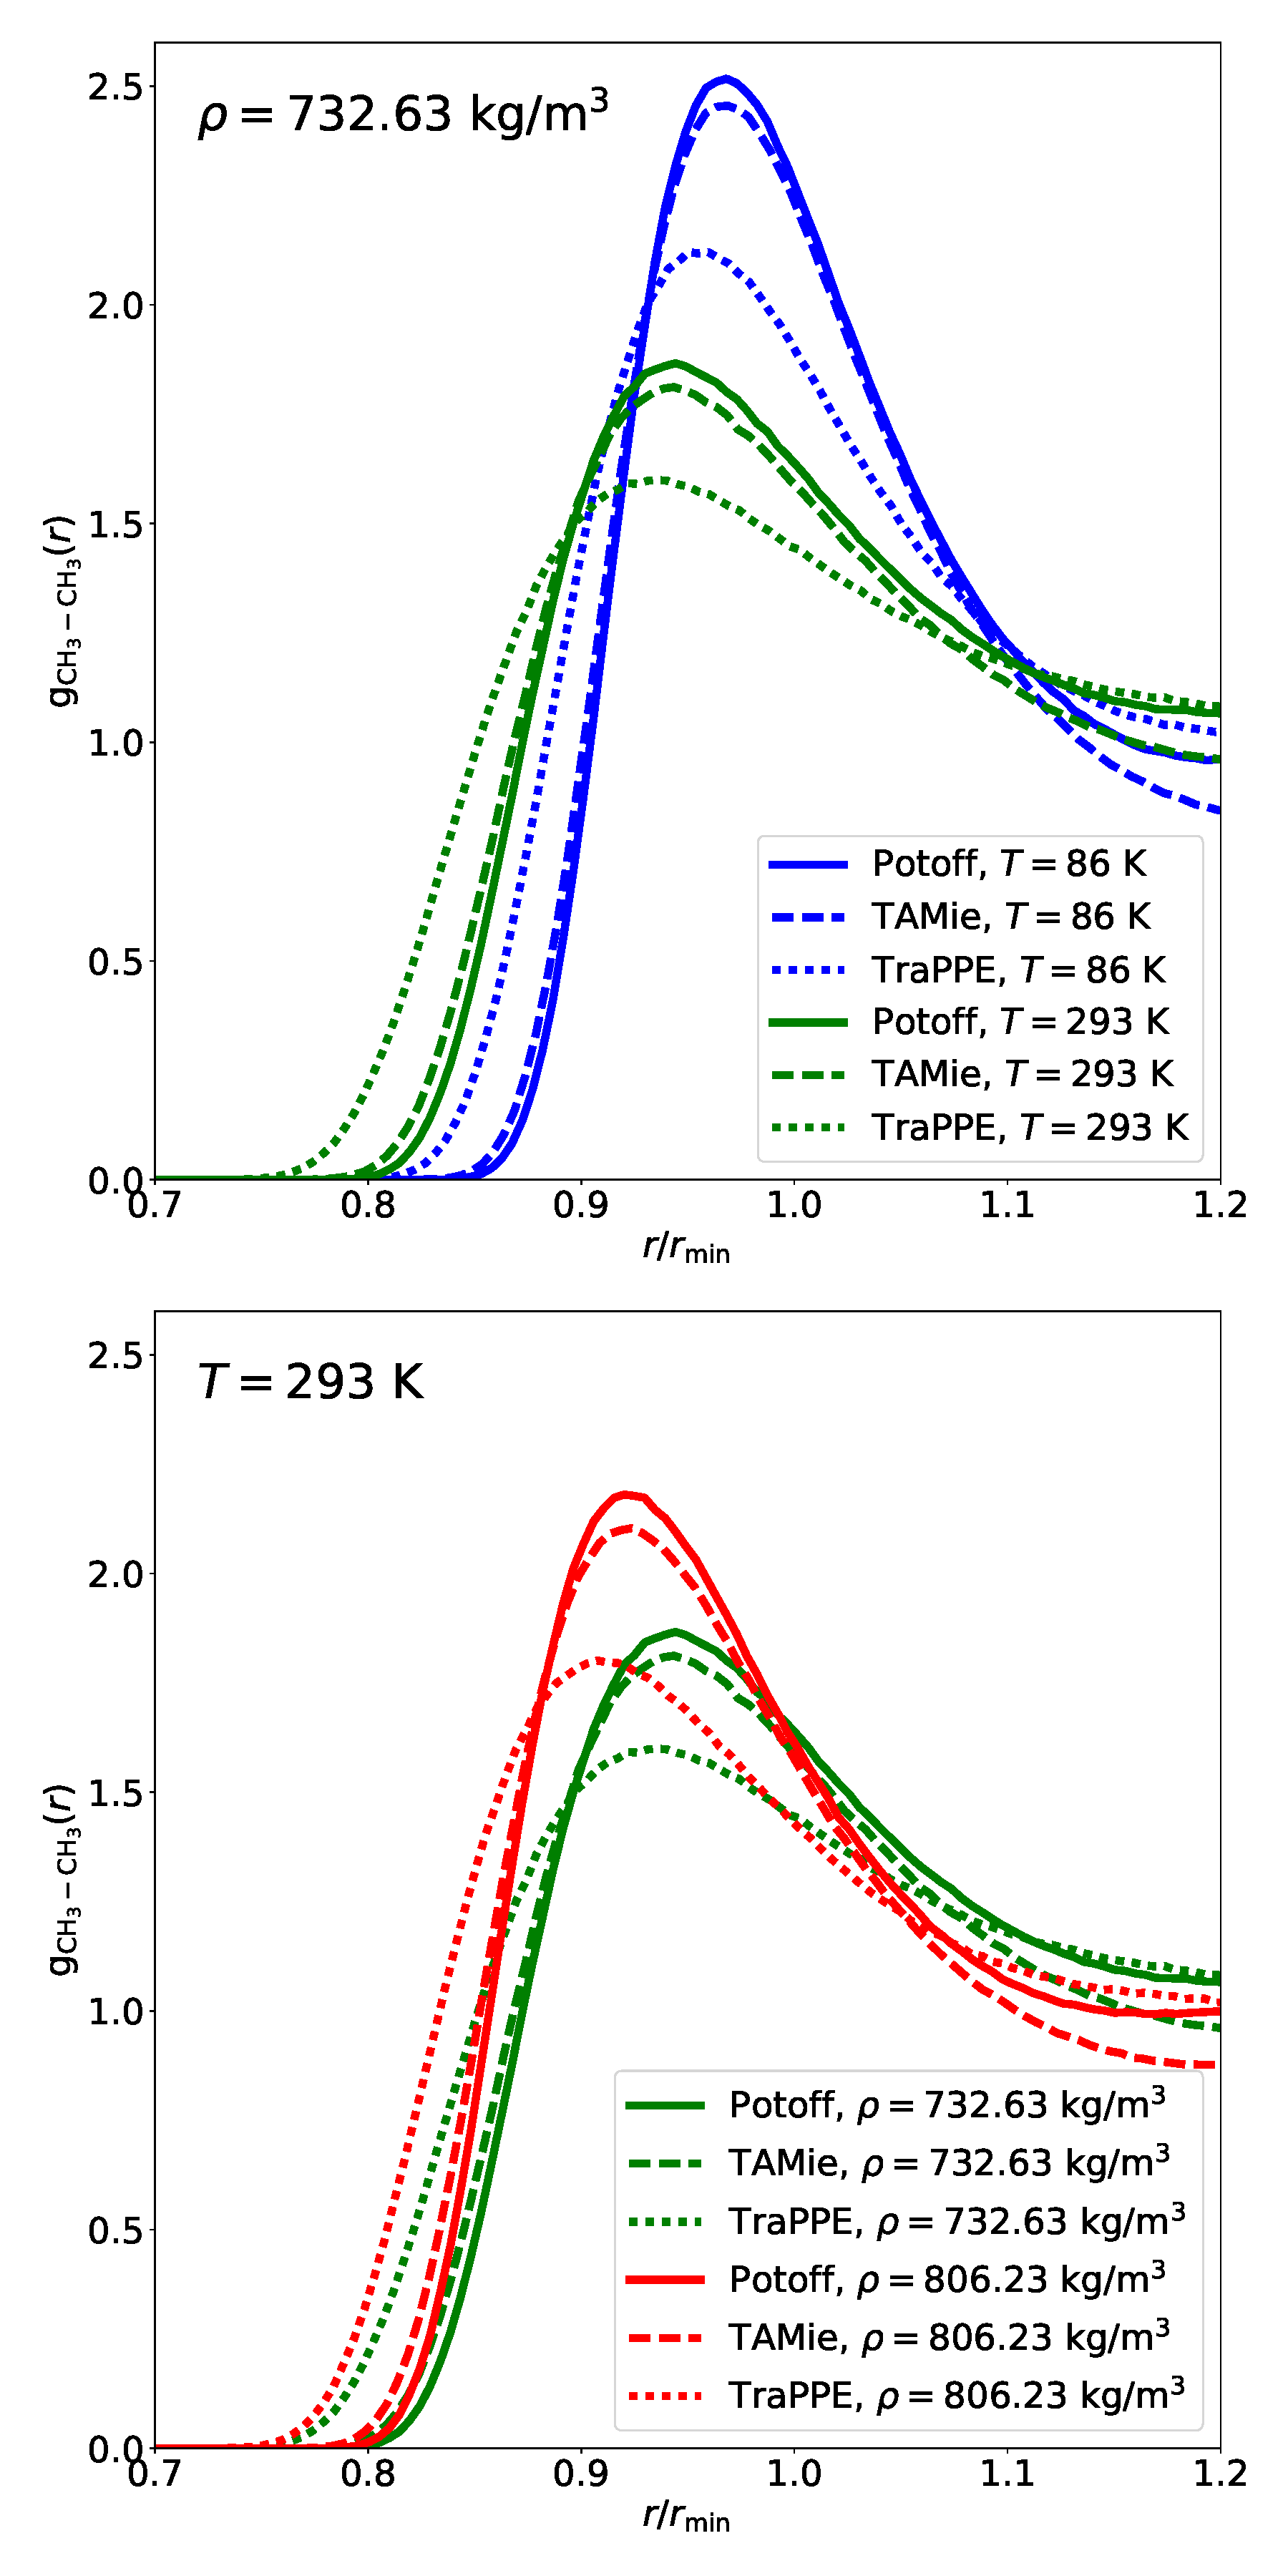
\includegraphics[width=3.2in]{RDF_comparison_CH3.pdf}
		\caption{Comparison of radial distribution function for CH$_3$-CH$_3$ interactions $(g_{\rm CH_3-CH_3}(r))$. The top panel compares two different temperatures along the triple point isochore. The bottom panel compares two different densities along the 293 K isotherm. Colors correspond to different state points while line styles denote different force fields.}
		\label{fig:RDF_comparison_CH3}
	\end{figure} 
	
	The top panel of Figure \ref{fig:RDF_comparison_CH3} demonstrates that the RDF shifts to the left (closer interactions) when increasing the temperature from 86 K to 293 K. Although the magnitude of this shift is similar for all three force fields, the Potoff viscosities appear to be impacted the most due to the steepness of the Mie 16-6 potential. By contrast, the bottom panel demonstrates that increasing the density at constant temperature does not shift the RDF, although it does increase the frequency of close-range interactions. Therefore, the overly repulsive Mie 16-6 potential is only problematic at high densities if there is sufficient thermal energy for the system to sample extremely close-range interactions. This explains why the Potoff force field is reliable near the triple point but significantly over estimates $\eta$ for high density systems at 293 K.
	
	% at high densities along the saturation curve but over estimates the $\eta$-$\rho$ dependence at 293 K.	
	
	%Therefore, It is clear from Figure \ref{fig:RDF_comparison_CH3} that the higher pressure simulations sample from much closer interactions than the triple point and, therefore, these close interactions cause the over estimation of compressed liquid viscosities but not saturated high density liquid viscosities.
	
	% This effect is due to the low thermal energy available near the triple point temperature. 
	
%	\begin{enumerate}
%		\item Finite-size effects
%		\item Fixed vs flexible bonds
%		\item Simulation time, high viscosities
%		\item Cut-offs for C12
%		\item RDFs for propane
%	\end{enumerate}
%	
%	\begin{enumerate}
%		\item Discussion
%		\begin{enumerate}
%			\item Mie potentials parameterized with VLE data provide significant improvement over LJ 12-6
%			\item Potoff over predicts $\eta-\rho$ dependence while TAMie is fairly accurate
%			\item Potoff appears to be slightly more accurate for $\eta-P$
%			\item Branched alkanes are not as accurate, perhaps assumption of transferability or torsional parameters
%		\end{enumerate}
%		\item Limitations
%		\begin{enumerate}
%			\item Largest viscosity simulations are slow to converge and unclear if simulations are sufficiently long
%			\item Tail-corrections could impact dynamics
%			\item Using REFPROP saturation conditions instead of force fields
%		\end{enumerate}
%	\end{enumerate}

	\subsection{Finite-size effects}

	Although finite-size effects are often assumed to be negligible for viscosity estimates with equilibrium molecular dynamics, ``Best Practices'' recommends validating this assumption by plotting $\eta$ with respect to $N^{-1/3}$. Figure \ref{fig:finite_size_effects} compares simulation results for 100, 200, 400, and 800 molecule systems. While Figure \ref{fig:finite_size_effects} only presents results for propane, we also observe similar results for a larger compound, specifically, 2,2,4-trimethylpentane.
	
	%Previous studies have demonstrated that finite-size effects are often negligible for viscosity estimates with equilibrium molecular dynamics.
	
	%However, since this analysis is typically not reported in the literature, the ``Best Practices'' guide recommends validating that finite-size effects are indeed negligible. For this reason,
	
	%The dashed lines are averages of the four system sizes while the solid line is a linear fit with respect to $N^{-1/3}$.   
	
	\begin{figure}[htb!]
		\centering
		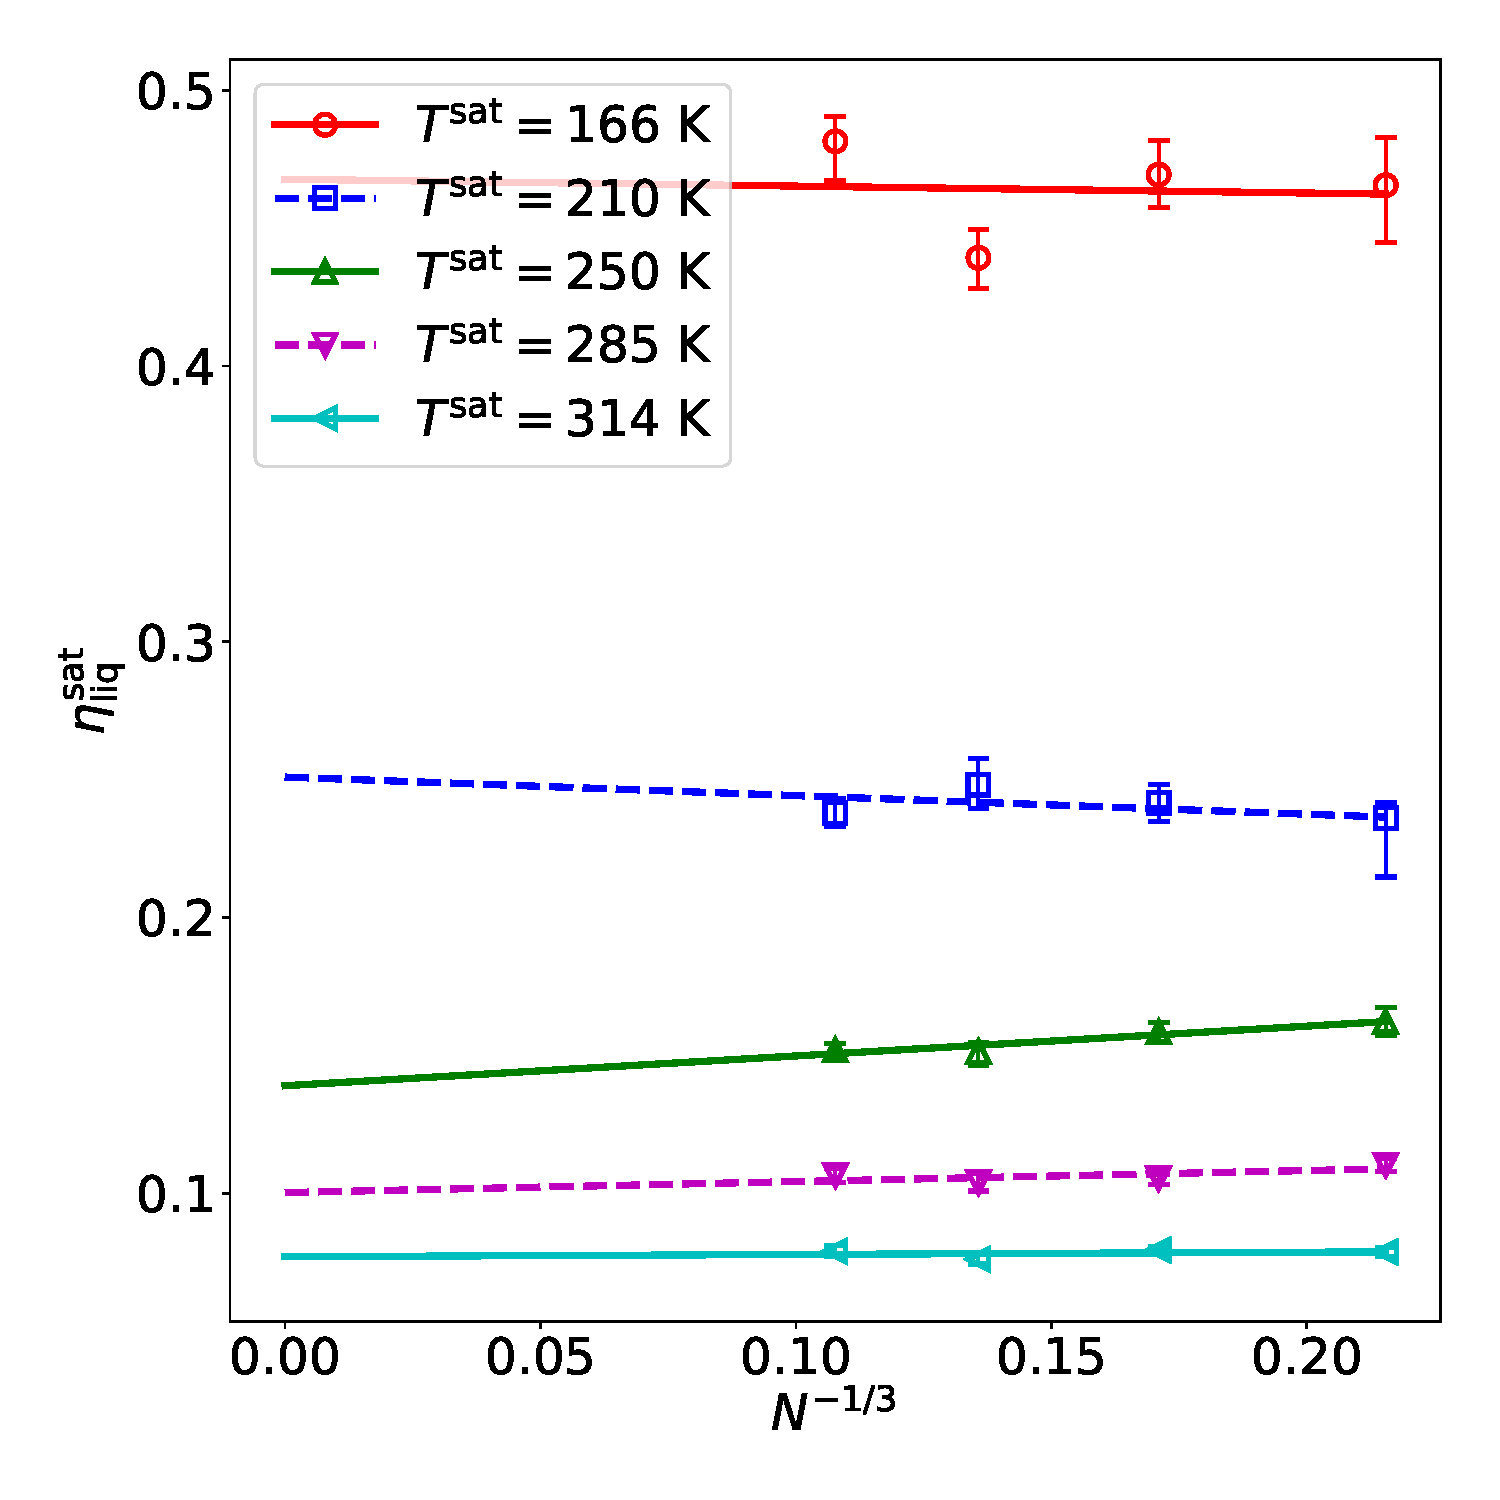
\includegraphics[width=3.2in]{C3H8_Potoff_finite_size_effects.pdf}
		\caption{Finite-size effects. Simulation results were obtained for propane with the Potoff force field and $N= 100$, $200$, $400$, and $800$. Colors/symbols denote different saturation temperatures. The lines are obtained from a weighted linear fit with respect to $N^{-1/3}$.}
		\label{fig:finite_size_effects}
	\end{figure} 
	
	Notice that the averages and uncertainties are typically quite similar for the different values of $N$, although some clear exceptions exist, e.g., $N = 800$ and $N=400$ for $T = 166$ K. Although the uncertainties do not overlap in all cases, there does not appear to be a consistent trend for the average $\eta$ with respect to $N^{-1/3}$. Therefore, we do not attribute the lack of overlap between certain systems to finite-size effects. Rather, this demonstrates the difficulty in obtaining completely reproducible values with the EMD Green-Kubo methodology, even when following ``Best Practices.'' Furthermore, note that extrapolating to $N^{-1/3} \rightarrow 0$, i.e., $N \rightarrow \infty$, can result in unrealistic estimates of $\eta$. For these reasons, we do not recommend the linear fit and extrapolation approach to correct for finite-size effects.
	
	% by per extrapolating to $N \rightarrow \infty$. 
	
	% when extrapolating to  For these reasons, we do not recommend extrapolating to $N \rightarrow \infty$, i.e., $N^{-1/3} \rightarrow 0$, as this tends to introduce unrealistic deviations.
	
	%Notice that the averages and uncertainties typically overlap considerably. Since there is no clear trend with respect to $N^{-1/3}$, we do not recommend extrapolating to $N^{-1/3} \rightarrow 0$, i.e., $N \rightarrow \infty$. 
	
	%%% This method did not appear to be useful in the end
	
%	In addition to this visual inspection, we also perform a ``hypothesis test'' to determine if the results from different system sizes are statistically indistinguishable. We utilize the following ``random permutation test'' \cite{BLANK}:
%	
%	\begin{enumerate}
%		\item Compute the ``observed'' sum-of-squares between the four different system sizes $(SS_{\rm obs})$
%		\item Randomly divide all of the replicate simulations (regardless of system size) into four groups, ``A'', ``B'', ``C'', and ``D'' \label{item:shuffling}
%		\item Average the replicate Green-Kubo integrals of each group \label{item:averaging}
%		\item Fit Equation \ref{eq: Double exponential} to the averages from Step \ref{item:averaging} \label{item:fitting}
%		\item Calculate the ``permutated'' sum-of-squares between the four different groups $(SS_{\rm perm}$ \label{item:SS_ABCD}
%		\item Repeat Steps \ref{item:shuffling} to \ref{item:SS_ABCD} hundreds of times $(N_{\rm perm})$
%		\item Count the number of permutations where $SS_{\rm perm} > SS_{\rm obs}$ $(N_{\rm rej})$ \label{item:counting}
%		\item Assign a $p$-value equal to the ratio of $N_{\rm rej}$ divided by $N_{\rm perm}$
%		\item If $p > 0.05$, we fail to reject the Null-hypothesis that all four system sizes are statistically equivalent, i.e., finite-size effects are likely negligible
%	\end{enumerate}
%
%	This approach is employed in place of the standard Analysis of Variance (ANOVA) test because it is not possible to compute a reliable $F$-statistic. Computing the $F$-statistic requires the sum-of-squares between replicates, which is not well-defined because an individual replicate simulation does not provide a meaningful estimate of $\eta$. Therefore, we can only compute the sum-of-squares between averages and not the sum-of-squares between replicates. However, since the sum-of-squares between replicates is a constant value regardless of the grouping in Step \ref{item:shuffling}, comparing the sum-of-squares is equivalent to comparing the $F$-statistic.  
	
	%	\begin{enumerate}
	%		\item Compute the ``observed'' $F$-statistic between the four different system sizes $(F_{\rm obs})$
	%		\item Randomly divide the replicate simulations of each system size into two groups, ``A'' and ``B'' \label{item:shuffling}
	%		\item Average the replicate Green-Kubo integrals of both groups \label{item:averaging}
	%		\item Fit Equation \ref{eq: Double exponential} to the averages from Step \ref{item:averaging} \label{item:fitting}
	%		\item Calculate the $F$-statistic for the two different groups $(F_{\rm AB}$ \label{item:F_AB}
	%		\item Repeat Steps \ref{item:shuffling} to \ref{item:F_AB} hundreds of times $(N_{\rm perm})$
	%		\item Count the number of permutations with $F_{\rm AB} > F_{\rm obs}$ \label{item:counting}
	%		\item Divide the value obtained in Step \ref{item:counting} by $N_{\rm perm}$ 
	%	\end{enumerate}
	

	%	\begin{enumerate}
	%		\item Computing the difference between two different system size
	%		\item Randomly dividing the replicate simulations of each system size into two groups, ``A'' and ``B''
	%		\item Averaging the replicate Green-Kubo integrals of both groups \label{step:averaging}
	%		\item Fitting Equation \ref{eq: Double exponential} to the averages from Step \ref{step:averaging}
	%		\item Calculating the difference between $\eta^{\infty}_{\rm A}$ and $\eta^{\infty}_{\rm B}$ $(\Delta \eta_{\rm AB})$
	%		\item Repeating steps 2 to 5 hundreds of times
	%		\item Binning the distribution of $\Delta \eta_{\rm AB}$ values
	%		\item Comparing the 
	%	\end{enumerate}
	
	%	 randomly dividing the replicate simulations of each system size into two groups, ``A'' and ``B,'' computing the average Green-Kubo integral for both groups, fitting Equation \ref{eq: Double exponential} for both averages, calculating the difference between $\eta^{\infty}_{\rm A}$ and $\eta^{\infty}_{\rm B}$, repeating this process hundreds of times, and  selecting a subset of replicate simulations from each system size and computing the average.
	
	%	\begin{enumerate}
	%		\item Simulation results for 100, 200, 400, and 800 molecules
	%	\end{enumerate}
	
	\subsection{Cut-off distance}
	
	The choice of cut-off distance is a subtle but important decision. In this study, we implement a 1.4 nm cut-off for TraPPE, TraPPE-2, TAMie, and AUA4 but a 1.0 nm cut-off for Potoff, as these are the cut-off lengths implemented by the respective authors.
	
	% each force field except Potoff, which utilizes only a 1.0 nm cut-off. This choice was made because the Potoff force field was parameterized with a 1.0 nm cut-off. 
	
	The ``Best Practices'' guide suggests that cut-off lengths could impact viscosity estimates but does not provide any support for this claim. To address this issue, we perform simulations with the Potoff force field using three different cut-off distances. Specifically, Figure \ref{fig:cutoff_distance} presents the Potoff $\eta_{\rm liq}^{\rm sat}$ values for \textit{n}-butane, \textit{n}-octane, and \textit{n}-dodecane using cut-offs of 1.0 nm, 1.4 nm, and 1.8 nm. 
	
	% convincing evidence to prove or disprove this notion.
	
	\begin{figure}[htb!]
		\centering
		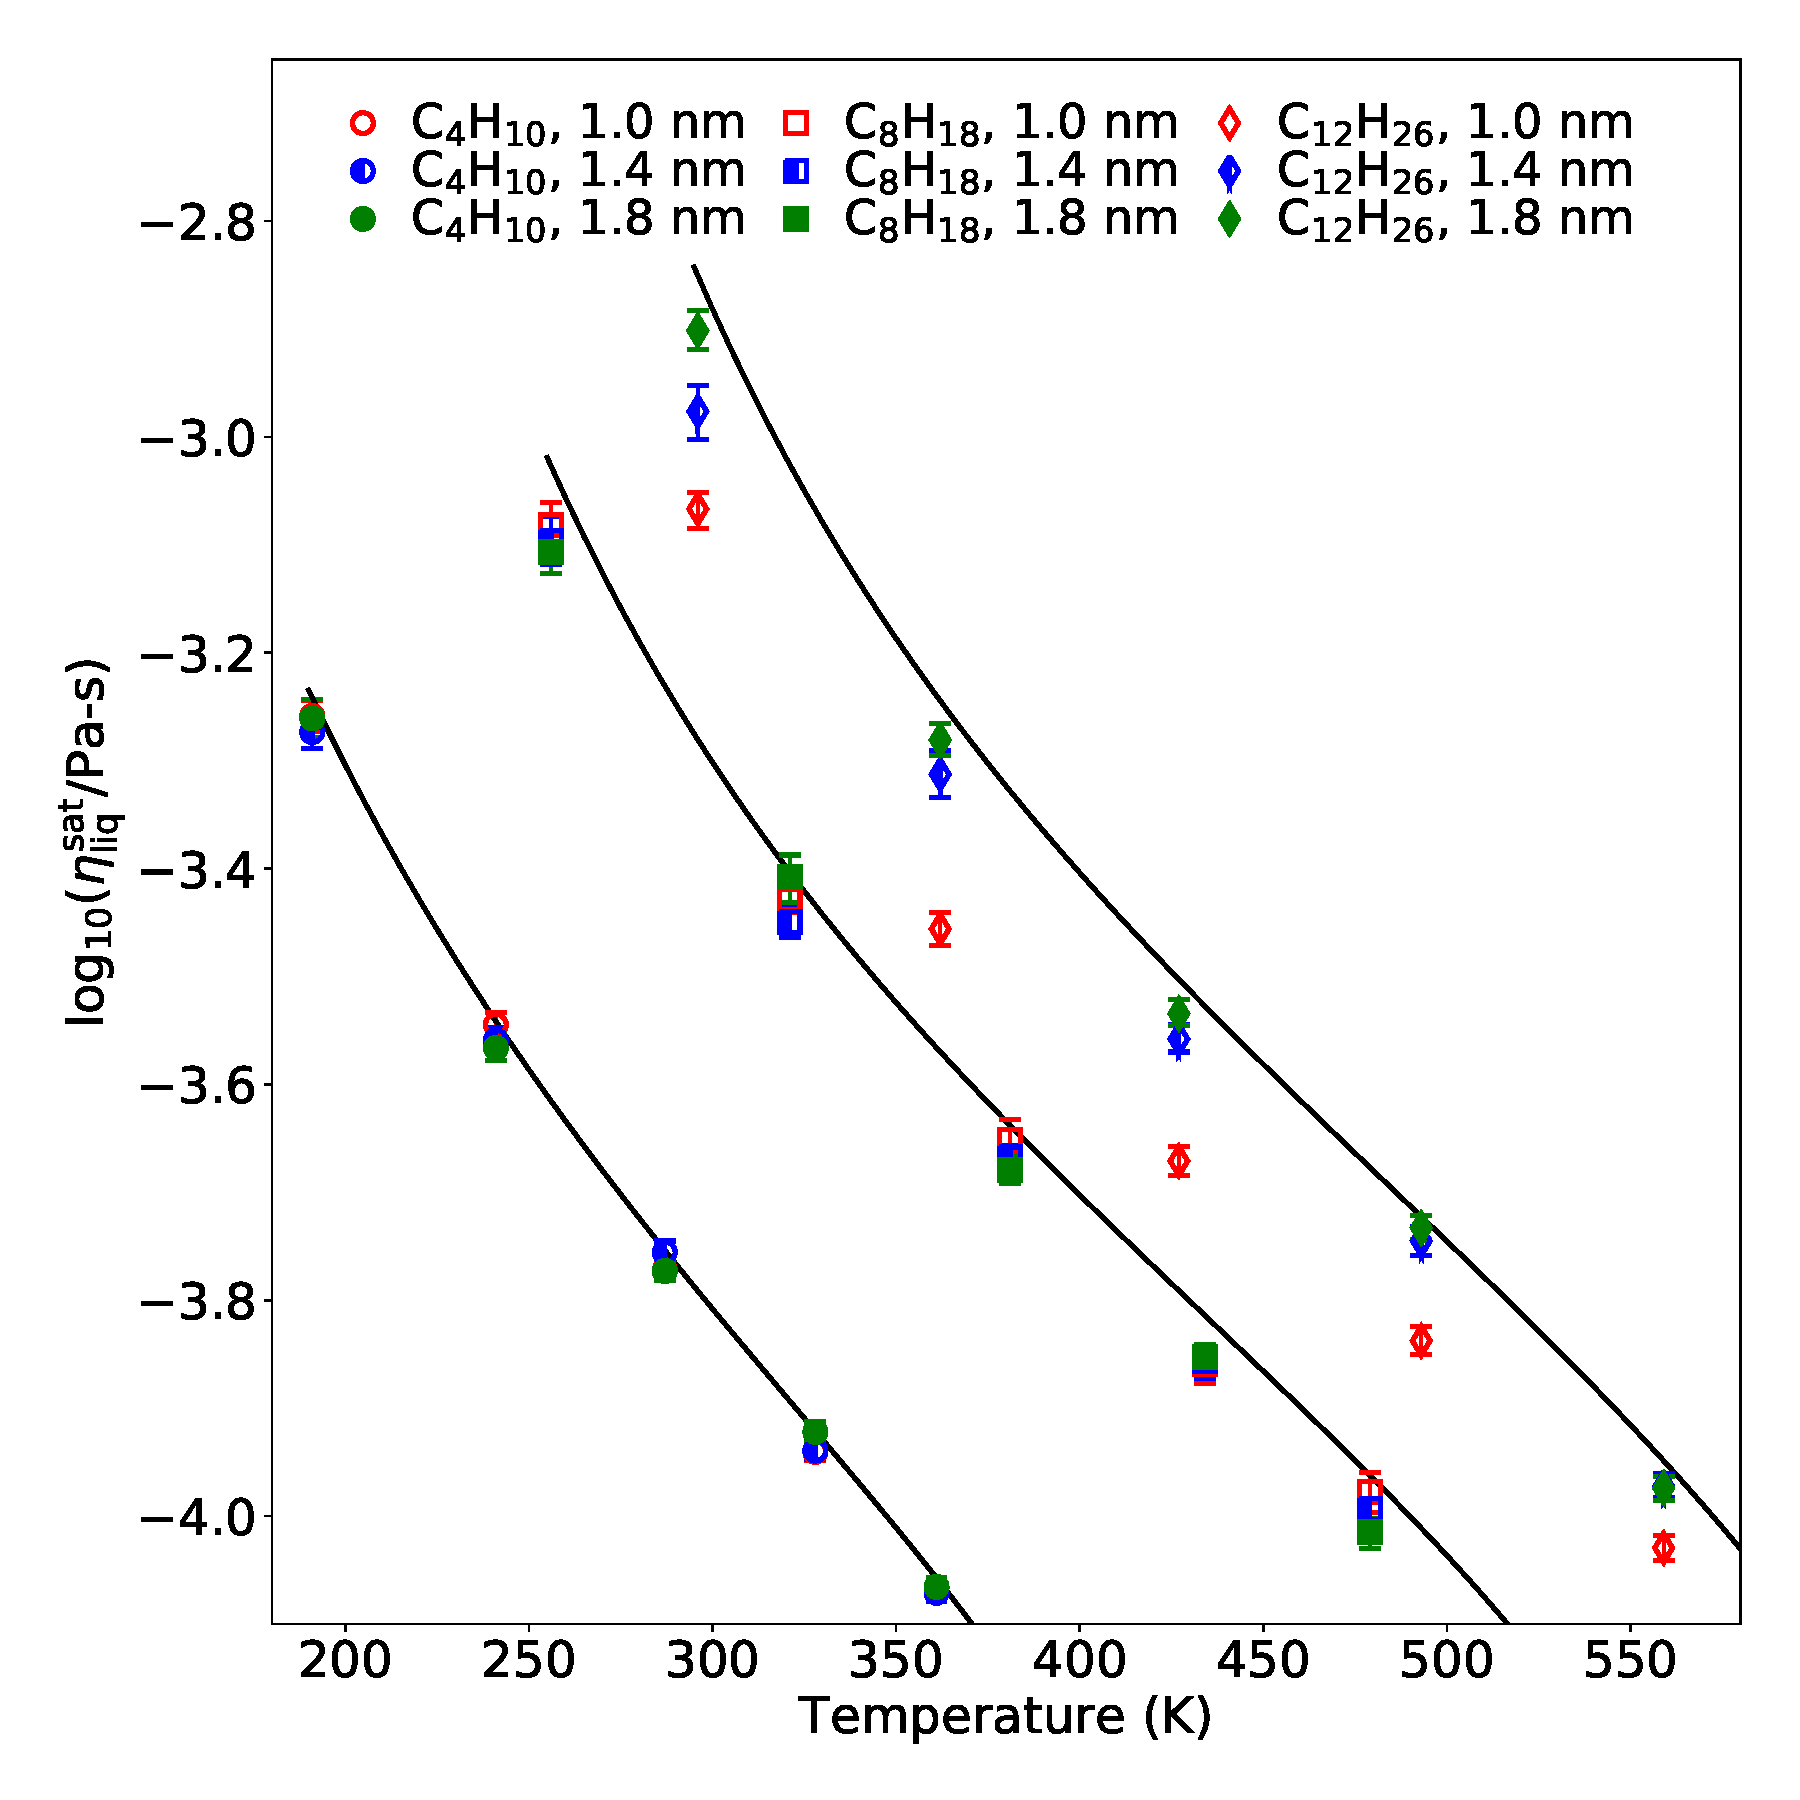
\includegraphics[width=3.2in]{cutoff_distance.pdf}
		\caption{Impact of cut-off distance. Colors/symbols denote different cut-off lengths. Different shapes correspond to \textit{n}-butane, \textit{n}-octane, and \textit{n}-dodecane. REFPROP values are provided as a visual reference. Simulations are performed with Potoff force field at saturation conditions.}
		\label{fig:cutoff_distance}
	\end{figure} 

%	Figure \ref{fig:cutoff_distance} demonstrates that for smaller compounds the impact of cut-off is negligible. For larger compounds, such as \textit{n}-dodecane, a 1.0 nm cut-off leads to significant error. In fact, \textit{n}-hexadecane and \textit{n}-docosane were unstable with a 1.0 nm cut-off and a 2 fs time-step. Reducing the time step to 1 fs was capable of stabilizing the 1.0 nm cut-off, but would require twice the computational time. Note that even the 1.4 nm cut-off results are not identical to those with a 1.8 nm cut-off. However, since the computationally expensive operation of computing pair interactions is proportional to the square of the cut-off, the 1.8 nm cut-off increases the simulation wall-time by nearly a factor of two compared to the 1.4 nm cut-off. For these reasons, the Potoff results for \textit{n}-dodecane, \textit{n}-hexadecane, and \textit{n}-docosane presented previously in Figure \ref{fig:Saturation_C12_C16_C22} were actually obtained using a 1.4 nm cut-off.
%
%    Recall in Figure \ref{fig:Saturation_C12_C16_C22} that the longer \textit{n}-alkanes demonstrate a temperature dependent deviation for the Potoff force field, which was not observed for smaller compounds. Based on the results in Figure \ref{fig:cutoff_distance}, we propose that this deviation is not a limitation in the force field, but rather is an artifact of the cut-off length.
%	
%	Figure \ref{fig:cutoff_distance} demonstrates that for smaller compounds the impact of cut-off is negligible. For larger compounds, such as \textit{n}-dodecane, a 1.0 nm cut-off leads to significant error. Even the 1.4 nm cut-off results are not identical to those with a 1.8 nm cut-off for \textit{n}-dodecane. Recall in Figure \ref{fig:Saturation_C12_C16_C22} that the longer \textit{n}-alkanes demonstrate a temperature dependent deviation for the Potoff force field, which was not observed for smaller compounds. Based on the results in Figure \ref{fig:cutoff_distance}, we propose that this deviation is not a limitation in the force field, but rather is an artifact of the cut-off length.
%
%    These results are somewhat troubling, since the computationally expensive operation of computing pair interactions is proportional to the square of the cut-off. Therefore, the 1.8 nm cut-off increases the simulation wall-time by nearly a factor of two compared to the 1.4 nm cut-off.
%	
%	In fact, \textit{n}-hexadecane and \textit{n}-docosane were unstable with a 1.0 nm cut-off and a 2 fs time-step. Reducing the time step to 1 fs was capable of stabilizing the 1.0 nm cut-off, but would require twice the computational time.  For these reasons, the Potoff results for \textit{n}-dodecane, \textit{n}-hexadecane, and \textit{n}-docosane presented previously in Figure \ref{fig:Saturation_C12_C16_C22} were actually obtained using a 1.4 nm cut-off.
%	
	Figure \ref{fig:cutoff_distance} demonstrates that for smaller compounds (\textit{n}-butane and \textit{n}-octane) the impact of cut-off is negligible. For larger compounds, however, such as \textit{n}-dodecane, a 1.0 nm cut-off leads to significant error. Unfortunately, Figure \ref{fig:cutoff_distance} demonstrates that even the 1.4 nm cut-off results are not identical to those with a 1.8 nm cut-off for \textit{n}-dodecane. 
	
	Recall in Figure \ref{fig:Saturation_C12_C16_C22} that the longer \textit{n}-alkanes demonstrate a temperature dependent deviation for the Potoff (and TAMie) force field, which was not observed for smaller compounds. Based on the results in Figure \ref{fig:cutoff_distance}, we propose that this deviation is not a limitation in the force field, but rather is an artifact of the cut-off length. This is somewhat troubling, since the computationally expensive operation of computing pair interactions is proportional to the square of the cut-off. For example, the 1.8 nm cut-off increases the simulation wall-time for these systems by nearly a factor of two compared to the 1.4 nm cut-off.
	
	In addition, \textit{n}-hexadecane and \textit{n}-docosane were unstable with a 1.0 nm cut-off and a 2 fs time-step. Reducing the time step to 1 fs was capable of stabilizing the 1.0 nm cut-off, but would require twice the computational time and does not resolve the observed bias. As a compromise between stability, speed, and accuracy, the Potoff results for \textit{n}-dodecane, \textit{n}-hexadecane, and \textit{n}-docosane presented previously in Figure \ref{fig:Saturation_C12_C16_C22} were actually obtained using a 1.4 nm cut-off.
		
	%For this reason, the Potoff results for \textit{n}-dodecane, \textit{n}-hexadecane, and \textit{n}-docosane presented previously in Figure \ref{fig:Saturation_C12_C16_C22} were actually obtained using a 1.4 nm cut-off.
	
	%, and even a 1.4 nm cut-off demonstrates some small deviations
	
%	  while a 1.0 nm cut-off causes a significant error for \textit{n}-dodecane.
	
%	In fact, \textit{n}-hexadecane and \textit{n}-docosane were unstable with a 1.0 nm cut-off and a 2 fs time-step. Reducing the time step to 1 fs was capable of stabilizing the 1.0 nm cut-off, but would require twice the computational time. 
	
	The instability of a 1.0 nm cut-off (with 2 fs time-steps) and the discrepancy in $\eta$ values obtained with different cut-offs demonstrate the importance of verifying that the cut-off distance is long enough to not impact the system dynamics. Furthermore, this demonstrates a scenario where alternative tail modifications may be preferable, e.g., force-shift or switch-force \cite{GROMACS_2018}. Unfortunately, these tail modifications significantly impact saturation properties, suggesting that the non-bonded parameters must be re-optimized with the tail modification \cite{Thol_LJTS,Thol2016_LJ}. Therefore, performing simulations with a force-shift or switch-force potential for Potoff, TraPPE, TAMie, and AUA4 would likely result in inaccurate viscosities. Re-parameterizing the non-bonded interactions for a force-shift or switch-force potential is beyond the scope of this study.
	
	\subsection{$\rho_{\rm liq}^{\rm sat}$}
	
	The use of REFPROP $\rho_{\rm liq}^{\rm sat}$ instead of the force field $\rho_{\rm liq}^{\rm sat}$ can lead to meta-stable simulations and spurious results. This occurs when the force field $P_{\rm vap}^{\rm sat}$ is less than the REFPROP $P_{\rm vap}^{\rm sat}$. Fortunately, this is uncommon since Potoff, TAMie, AUA4, and TraPPE-2 are quite reliable for estimating $P_{\rm vap}^{\rm sat}$ and TraPPE significantly over estimates $P_{\rm vap}^{\rm sat}$. Furthermore, even the lowest temperature simulations of propane did not appear to be below the melting point for each force field, i.e., the RDFs were liquid-like (cf. top panel of Figure \ref{fig:RDF_comparison_CH3}). 
	
	There are at least four reasons why we perform simulations at the REFPROP $\rho_{\rm liq}^{\rm sat}$ instead of the force field $\rho_{\rm liq}^{\rm sat}$. First, this approach allows for a fair comparison of the force fields' ability to predict viscosity, without penalizing force fields which are less accurate at predicting $\rho_{\rm liq}^{\rm sat}$ or rewarding force fields that mask their deficiencies in predicting viscosity by over- or under estimating $\rho_{\rm liq}^{\rm sat}$.
	Second, this facilitates comparing force fields over the entire range of saturation temperatures, whereas this is extremely challenging using standard simulation methods for determining vapor-liquid saturation densities, such as Gibbs Ensemble Monte Carlo (GEMC) or Grand Canonical Monte Carlo (GCMC) histogram reweighting (HR). Third, it is straightforward to, at least qualitatively, account for a systematic deviation between the force field and REFPROP $\rho_{\rm liq}^{\rm sat}$, e.g., a positive bias in $\rho_{\rm liq}^{\rm sat}$ will increase $\eta_{\rm liq}^{\rm sat}$. Fourth, since each of the studied force fields utilized $\rho_{\rm liq}^{\rm sat}$ data in their optimization, deviations between the REFPROP and force field values are small, typically less than 1~\% (see Table 1 of Reference \citenum{Potoff_branched}). 
	
	However, due to the exponential dependence of $\eta$ on $\rho$, small differences in density can result in relatively large deviations in viscosity. For this reason, we perform a small set of validation simulations to determine the variability caused by utilizing the REFPROP densities. Specifically, we simulate \textit{n}-butane with Potoff, TraPPE, and TAMie and 3-methylpentane using Potoff and TraPPE. The saturated liquid densities for these validation runs were taken from the literature \cite{Martin1999,Mie,Potoff_branched,TAMie}, where Reference \citenum{Martin1999} utilized GEMC and References \citenum{Mie,Potoff_branched,TAMie} used GCMC-HR.      
	
	The results using the ``true'' force field $\rho_{\rm liq}^{\rm sat}$ for \textit{n}-butane and 3-methylpentane are found in Figures \ref{fig:Saturation_C3_C4_C8} and \ref{fig:Saturation_long_branched}, respectively, as filled symbols. Note that the Potoff, TAMie, and TraPPE \textit{n}-butane and TraPPE 3-methylpentane filled points are consistent with the respective empty points. This is due to the good agreement between the force field $\rho_{\rm liq}^{\rm sat}$ and the REFPROP $\rho_{\rm liq}^{\rm sat}$ (less than 0.3~\%). By contrast, the Potoff 3-methylpentane filled point is approximately 3~\% lower than the respective empty points. This is because the Potoff force field under estimates $\rho_{\rm liq}^{\rm sat}$ by around 1.15~\% \cite{Potoff_branched}. In comparison, the Potoff S/L deviations in $\rho_{\rm liq}^{\rm sat}$ are between -0.12~\% and -0.60~\% for all other branched compounds studied. TraPPE deviations in $\rho_{\rm liq}^{\rm sat}$ are less than $\pm$ 0.6~\% for all compounds except for 2,2-dimethylpropane and 2,2,4-trimethylpentane, which have -1.55~\% and 2.81~\% deviations, respectively. Therefore, utilizing the actual force field $\rho_{\rm liq}^{\rm sat}$ values would not alter the qualitative trends observed in Figures \ref{fig:Saturation_Ethane} to \ref{fig:Saturation_long_branched} and should only modify the quantitative values by a few percent in most cases and not more than 10~\% in the most extreme cases.     
	
%	, are less reliable near the triple point. By utilizing REFPROP densities, it is possible to compare force fields over the entire range of saturation temperatures.
	
	\section{Conclusions} \label{Conclusions}
	
	This study demonstrates the improvement that has taken place over the past two decades for predicting viscosity with molecular simulation. First, the ``Best Practices'' for EMD lead to more reproducible results. Second, the state-of-the-art Mie $\lambda$-6 force fields are significantly more accurate than the traditional Lennard-Jones 12-6 force fields for viscosity, as well as for vapor-liquid coexistence properties. More specifically, the Potoff and TAMie force fields typically predict saturated liquid viscosities for \textit{n}-alkanes to within 10~\% of the REFPROP values. By contrast, the TraPPE and AUA4 models under predict saturated liquid viscosities by 20~\% to 50~\%, where the deviations are largest at lower temperatures. While Potoff and TAMie are also more reliable for branched alkanes, deviations are larger and demonstrate a similar temperature dependence. 
	
	The key limitation of the Potoff force field is that the choice of $\lambda = 16$ is too repulsive at close distances, which causes the viscosity to be over estimated at high densities. Due to a fortuitous cancellation of errors, the Potoff potential does provide a reliable $\eta$-$P$ trend. Since TAMie uses $\lambda =14$, the $\eta$-$\rho$ trend is slightly more reliable than that of Potoff. It is important to emphasize that transport properties were not included in the training set for parameterizing the Potoff and TAMie force fields. Therefore, the results from this study demonstrate that the improved prediction of static vapor-liquid coexistence properties obtained with Mie $\lambda$-6 potentials also results in improved prediction of liquid viscosity, a dynamic property.
	
	% liquid viscosity. a transport property, namely, liquid viscosity.
	
	\section*{Supporting Information}
	
    Section \ref{Gromacs input files} provides GROMACS input files.	Section \ref{Systems simulated} enumerates all systems simulated. Section \ref{Additional simulation details} details the MD integrator, thermostat, and barostat. Section \ref{SI:Simulation time} compares simulation results with varying production times. Section \ref{fixed flexible} determines the sensitivity of our results to the use of fixed bonds. Section \ref{SI:GK_analysis} outlines the Green-Kubo analysis process. Section \ref{Validation Runs} validates our methods by comparing with reference simulation values. Section \ref{SI:Tabulated} contains tabulated simulation values.       
	
	\section*{Acknowledgments}
	
	We are grateful for the internal review provided by Andrei F. Kazakov and Alta Y. Fang of the National Institute of Standards and Technology (NIST). This research was performed while Richard A. Messerly held a National Research Council (NRC) Postdoctoral Research Associateship at NIST and while Michelle C. Anderson held a Summer Undergraduate Research Fellowship (SURF) position at NIST. Contribution of NIST, an agency of the United States government; not subject to copyright in the United States.
	
	\bibliographystyle{unsrt}
	\bibliography{Special_issue_references}
		
\end{document}
